\documentclass{ufpatcc}

\include{include}
%% Packages used for the TCC

%\usepackage{booktabs}

%%%% Definitions and New commnads %%%%

\newcommand{\sen}{\operatorname{sen}}
\newcommand{\mbeq}{\overset{!}{=}}

\renewcommand\Re{\operatorname{Re}}
\renewcommand\Im{\operatorname{Im}}

%%%% New control sequences %%%%

\newcommand{\redeq}[1] {\textcolor{red}{#1}}
\newcommand{\blueeq}[1] {\textcolor{blue}{#1}}
\newcommand{\att}[1] {\textcolor{red}{#1}}
% Used Packages:
\usepackage{tikz}
\usepackage{float}
\usepackage{steinmetz}
\usetikzlibrary{arrows,shapes,shapes.multipart}
%\usepackage[brazil]{babel}
\usepackage[T1]{fontenc}
\usepackage[utf8]{inputenc}
\usepackage{amsmath}
\usepackage{amsfonts}
\usepackage{enumitem} % To adjust lists
\usepackage{verbatim} % Multi-line comments
\usepackage{mathabx} % Package that contains the circular convolution symbol
\usepackage{graphicx}
\usepackage{caption}
\usepackage{subcaption}
\usepackage{units}
\usepackage{adjustbox}
\usepackage{dirtytalk}
\usepackage{csquotes}

%\usepackage[backend=bibtex8]{biblatex}

\ifpdf

\ifdefined\hyperref
\else
\usepackage[pdftex,colorlinks]{hyperref}
\fi

\hypersetup{%
pdftitle={Some title},
pdfauthor={Your name - LaPS - UFPA},
pdfkeywords={DSP,Signal},
pdfstartview={FitH}, %% <--
urlcolor=black,
%linkcolor=blue,
linkcolor=black,
%citecolor=red,
citecolor=black,
}

% Ensiar o Latex a separar silabas
\hyphenation{DMT En-ge-nhei-ro}


\ufpaTitulo{An FPGA-Based Radio Frontend for LTE Transmission on Cloud RAN}

\ufpaAutor{Gabriel Peixoto de Carvalho}
\ufpaSegundoAutor{}
\ufpaOrientador{Prof. Aldebaro Barreto da Rocha Klautau Junior}
\ufpaCoordenadorCurso{Prof. Francisco Carlos Bentes Frey Muller}

\ufpaCoOrientador{Eng. Igor Antonio Auad Freire}
\ufpaMembroBancaA{Prof. Francisco Carlos Bentes Frey Muller}
\ufpaMembroBancaB{Eng. Ilan Souza Correa}


\begin{document}

\ufpaPaginaDeRosto

\ufpaPagRostodo

\ufpaPaginaDeAprovacao

%%%%%%%%%%%%%%%%%%%%
%   Oferecimento   %
%%%%%%%%%%%%%%%%%%%%

\begin{ufpaOferecimento}
\index{Oferecimento@Oferecimento}%
\addcontentsline{toc}{chapter}{Dedicatoria}

\end{ufpaOferecimento}

%%%%%%%%%%%%%%%%%%%%
%  Agradecimento   %
%%%%%%%%%%%%%%%%%%%%

\begin{ufpaAgradecimentos}
\index{Agradecimentos@Agradecimentos}
\addcontentsline{toc}{chapter}{Agradecimentos}

\begin{flushright}
Gabriel Peixoto de Carvalho
\end{flushright}

\end{ufpaAgradecimentos}

%%%%%%%%%%%%%%%%%%%%
%      Epigrafe     %
%%%%%%%%%%%%%%%%%%%%

\begin{ufpaEpigrafe}
Viva como se voce fosse morrer amanha. Aprenda como se voce fosse viver para sempre.\\
\begin{flushright}Mahatma Gandhi\end{flushright}
\end{ufpaEpigrafe}

%%%%%%%%%%%%%%%%%%%%%
%  Lista de Siglas  %
%%%%%%%%%%%%%%%%%%%%%

\chapter*{List of Acronyms} \label{sec:siglas}
\begin{enumerate}
 \item ADSL - \textit{Linha de assinante digital assim�trica}
 %\item AWGN - \textit{Ru�do aditivo branco Gaussiano}
 %\item BER - \textit{Taxa de erro de bit}
 %\item DFT - \textit{Transformada de Fourier discreta}
 %\item DMT - \textit{Multi-tom discreto}
 %\item DSL - \textit{Linha de assinante digital}
 %\item FEQ - \textit{Equalizador em frequ�ncia}
 %\item FFT - \textit{Transformada rápida de Fourier}
 %\item FTTH - \textit{Fibra até a residência}
 %\item G.fast - \textit{Acesso rápido aos terminais do assinante}
 %\item ICI - \textit{Interferência inter-portadora}
 %\item IDFT - \textit{Transformada de Fourier discreta inversa}
 %\item IFFT - \textit{Transformada rápida de Fourier inversa}
 %\item ISI - \textit{Interferência inter-simbólica}
 %\item OFDM - \textit{Modulação por divisão ortogonal de frequência}
 %\item PC - \textit{Prefixo cíclico}
 %\item PSD - \textit{Densidade espectral de potência}
 %\item RIC - \textit{Resposta impulsiva do canal}
 %\item SC - \textit{Sufixo cíclico}
 %\item SER - \textit{Taxa de erro de símbolo}
 %\item SNR - \textit{Razão sinal ruído}
 %\item VDSL - \textit{Linha de assinante digital com taxa de bit muito alta}
 %\item 4GBB - \textit{Quarta geração de banda larga}
\end{enumerate}
 


\chapter*{List of Simbols} \label{sec:simbolos}
\begin{description}[labelsep=5em, align=left,labelindent=2cm]
\item[$\Delta f$] Spacing between subcarriers
\item[$N$]        Number of Symbols
\item[$n$]        Index of Subcarrier
\item[$a$]        Amplitude
\item[$m$]        Index of OFDM symbol
\item[$sm$]       Useful OFDM symbol
\item[$T_u$]      Period of symbol Generation
\item[$T_s$]      Period of OFDM symbols
%\item[$n_0$] Indice da amostra de início do símbolo recebido para o receptor sincronizado
%\item[$N$] Número de pontos da DFT ou tamanho do vetor símbolo DMT
%\item[$N_a$] Número de amostras afetadas por ISI e ICI
%\item[$p_k$] Parte real do $k$-ésimo subsímbolo
%\item[$P_x$] Potência total de transmissão
%\item[$q_k$] Parte imaginária do $k$-ésimo subsímbolo
%\item[$\mathbf{Q}$] Matriz DFT
\end{description}


%%%%%%%%%%%%%%%%%%%%%%%%%%%%%%%%%%%%%%%%%%%%
%  Insere a lista de Figuras e de Tabelas  %
%%%%%%%%%%%%%%%%%%%%%%%%%%%%%%%%%%%%%%%%%%%%

\listoffigures \clearpage \listoftables \clearpage

%%%%%%%%%%%%%%%%%%%%
%      Summary     %
%%%%%%%%%%%%%%%%%%%%

\tableofcontents    \clearpage

%%%%%%%%%%%%%%%%%%%%
%      Resumo      %
%%%%%%%%%%%%%%%%%%%%

\begin{ufpaResumo}

A evolu\c{c}\~{a}o do trafego nos servi\c{c}oes m\'{o}veis de voz para dados
modificou e vem modificando a forma como as tecnologias de acesso a r\'{a}dio e
suas camadas de aplica\c{c}\~{a}o s\~{a}o pensadas e implementadas. Atualmente o
t\'{o}pico de computa\c{c}\~{a}o em nuvem ou Cloud computing, vem sendo cada vez
mais recorrente, por causa de sua grande capacidade de escalar e criar um
sistema que seja perfeito para o tipo de aplica\c{c}\~{a}o do usu\'{a}rio.
Partindo dos dois conceitos citados anteriormente um paradigma no ramo das
tecnologias de acesso a r\'{a}dio vem gerando interesse nas operadoras, as redes
de acesso a radio centralizadas, ou em nuvem (C-RAN), com esse tipo de
tecnologia seria poss\'{i}vel escalar e alocar recursos dinâmicamente como todo
o poder que a computa\c{c}\~{a}o em nuvem proporciona e redirecionar esses
recursos para melhorar a qualidade das comunica\c{c}\~{o}es m\'{o}veis.

Como o conceito C-RAN \'{e} novo, logicamente surgem diversos questionamentos
acerca de como implementar e de que dispositivos ou tecnologias usar. Este
trabalho tem como objetivo avaliar um poss\'{i}vel setup de um fronthaul em LTE
que possa trabalhar de acordo com a demanda de reconfigurabilidade e
escalabilidade que o paradigma C-RAn necessita. Sendo este setup de um fronthaul
composto por dois dispositivos, uma FPGA (fronthaul digital) e um transceiver
(fronthaul anal\'{o}gico), ambos em combina\c{c}\~{a}o forma uma plataforma com
uma forte capacidade de reconfigura\c{c}\~{a}o em tempo-real.

O foco deste trabalho \'{e} a implementa\c{c}\~{a}o e a avalia\c{c}\~{a}o de sua
viabilidade, para tal o desenvolvimento come\c{c}ou com simples estudos das
plataformas em termos de controle e comunica\c{c}\~{a}o e vai at\'{e}
avalia\c{c}\~{a}o da comunica\c{c}\~{a}o. Este trabalho foi implementado usando
duas placas FPGA, primeiramente testado na placa ML605 com o chip FPGA Virtex-6
e ap\'{o}s o design foi portado para a placa VC707 com o chip FPGA Virtex-7 que
possu\'{i}a mais op\c{c}\~{o}es e perif\'{e}ricos interessantes para este
trabalho. O transceiver usado foi a placa FmcommS2 que possui capacidade de
múltiplas transmiss\~{o}es e recep\~{o}es (MIMO) e se conecta com a placa FPGA
atrav\'{e}s do conector FMC.

Neste trabalho foram estudados a integra\c{c}\~{a}o e controle do transceiver
pela FPGA, e ap\'{o}s isso o desenvolvimento de interfaces para transmiss\~{a}o
e recep\c{c}\~{a}o de dados, assim como os respectivos drivers e softwares
necess\'{a}rios para tal. O texto est\'{a} dividido em 5 partes totalizando 6
cap\'{i}tulos, a primeira parte \'{e} uma introdu\c{c}\~{a}o do trabalho, a
segunda parte trata de toda base te\'{o}rica utilizada no desenvolvimento, a
terceira parte \'{e} o núcleo do projeto onde v\~{a}o ser explicados as
funcionalidades dos dispositivos usados assim como todo o processo de
desenvolvimento estar\'{a} documentado nela. A quarta parte documenta os
resultados tanto de execu\c{c}\~{a}o quanto de simula\c{c}\~{a}o e os compara a
resultados esperados. A quinta e última parte trata das conclus\~{o}es e
poss\'{i}veis trabalhos futuros.

\end{ufpaResumo}

\begin{abstract}

The evolution of mobile services in terms of access technologies and application
layers is driving a huge change in mobile communication systems. A recent hot
topic in the field is the rise of the cloud computing paradigm, thus the idea
known as cloud radio access networks (Cloud-RAN) is growing in the industry.
This behavior comes from the potential of cloudfication for improvement in the
efficiency of resource allocation, manageability and power consumption, aspects
inherent of traditional RANs.

Thus, with the emerging of C-RAN, several questions about how to implement and
which tools to use come naturally. This work aims to evaluate the potential of a
programmable fronthaul radio interface, as known, actual network does not have
the adaptative capability needed for the C-RAN. For this work a setup of a radio
unit, composed by two fpgas (one acting as the Baseband unit and other as the
(digital front-end) of the radio unity) connected through ethernet and two
transceivers (analog front-end), one in each FPGA. Within this setup various
algorithms can be tested and can be evaluated in LTE scenarios because the
transceiver works in LTE and C-RAN.

This work shall focus on the evaluation of the radio interface and perform the
tests inherent to it, exploring FPGA adaptability and parallelism with the
internal and external communication protocols, and so exploring the advantages
of the transceiver used, the fmcomms2  development board (AD9361 chip) from
Analog devices, which is a device broadly used in software defined radio
hardwares, as known as USRPs (Universal Software Radio Peripheral).

An aspect of the transceiver that is very attractive to the C-RAN paradigm is
its configurability and scalability, capable of real-time adjustments in the
sampling frequency or operation mode from 2x2 to 4x4 MIMO (Multiple Inputs and
Multiple Outputs), this real-time adaptive characteristic is ideal to C-RAN
environment.

The results are generated primarily aiming a fidelity in the transmitted and
receiver signals, after these results are conclusive it is possible to proceed
to more complex tests and approaches of this setup. %Another test made was the
%analysis of the synchronization between  receiver and transceiver using a CIPRI
%emulator implemented in FPGA logic, which is the standard fronthaul interface,
%in this test it is possible to observe the advantages of the programmable radio
%front-end in the system.\\

\end{abstract}

%%%%%%%%%%%%%%%%%%%%%
%   Corpo do TCC    %
%%%%%%%%%%%%%%%%%%%%%

\pagenumbering{arabic}

\part{Introduction}
\chapter{Introduction}
\label{chap:intro}

The world is much more interconnected and the economy is growing wilder and
wilder, a lot of economical crisis rise in different countries almost every
year. The climate changes are also a concern to the modern governments, thus the
idea of re-utilizing resources and  make these resources be more economically
and environmentally friendly are a goal for modern research and development.\\

Cloud computing is a paradigm which is growing every year in the companies and
developers, it is not a magic method to solve all the problems but it solves
some infrastructure problems of small and big companies, where companies does
not need to won computers or anything locally to operate, everything can be done
remotely and a more experienced company and staff can offer such infrastructure
or application as a service. Such idea of having everything as a service is very
attractive both economically  and environmentally because there is no waste of
resource, everything is scalable to the need of the client and upgradeable if
needed.\\

The Radio access technologies have been evolving from audio traffic to
intensive data traffic over the recent standards, because the mobile devices
got a myriad of functions which could only be executed by Personal computers,
however the implementations of such networks demand a huge amount of resources
and with the economy becoming harder every year, there is the concern about how
to develop and deploy such networks and of course backwards compatibility of
these networks, because an operator would never deploy a network which is not
compatible with previous standards equipments, this is not profitable. Having
these ideas in mind the Centralized RAN idea began to be developed, such as
cloud computing, now there is the technology for the RANs to be scalable and
configurable to the needs of the clients and operators, where the baseband
processing is all done on the cloud and the radio front-ends are reconfigurable
to handle different data and modulation outputs.\\

The FPGA is very attractive to implement such radio front-ends and other
reconfigurable computing tasks, because it is flexible too be reconfigured
on-the-run and offers a really good processing and I/O capabilities. Thus this
work aims to evaluate the implementation feasibility of a radio front-end to
LTE transmissions (LTE band) in a Cloud RAN environment (adaptability and
reconfigurability).\\

This work is implemented in a Xilinx Virtex 7 FPGA and using the transceiver
FMComms2 from analog devices, this transceiver can be reconfigured in real time
and runs up to 6 GHz band, it has been chosen because of such reconfigurability
properties. This text is composed by 6 chapters divided in 5 parts.\\

The first part aims to introduce the environment in which this work was planned
with this introduction chapter. The second part is a literature review of
everything theoretical used in this work development, it is composed by two
chapters, the second chapter describing Cloud and Software defined radio
\ref{chap:sdr}, because this reconfigurability property has been widely
explored in software defined radio field. The third chapter is about Digital
communications and LTE, describing the basic blocks of digital communications
systems and briefly talking about LTE standard and how it is implemented
\ref{chap:lte}.\\

The third part is the core of the work, the implementation, in this chapter
the functionalities of both FPGA and transceiver shall be explained and the
work development will be described and how it was implemented in both FPGA
logic and software drivers \ref{chap:implementation}.\\

The fourth part reports all the results obtained in such work.The configuration
results report how the transceiver board communication and configuration were
succeed, the simulation results aim to show the VHDL blocks simulation prior to
hardware implementation and at last the transmission results \ref{chap:results}.

The last part is the conclusions and future works, which aim to report
everything learned from this work and what can be done to improve the
transmission/reception quality or communication \ref{chap:conclusion}.


\part{Literature Review}
\chapter{Software Defined Radio}

\section{Overview}
\label{sdr:overview}

As we could see in the previous chapter RAN as a service and cloud requires
devices which are both scalable and reconfigurable following customer demands,
in order to accomplish that there is a lot of schemes and theories involved, but
this work will focus on \emph{Software Defined Radio} which is defined according
to the \emph{SDR Forum} \cite{web:sdrforum} as:

say{radios that provide software control of a variety of modulation techniques,
wide-band or narrow-band operation, communications security functions (such as
hopping), and waveform requirements of current \& evolving standards over a
broad frequency range.}

In short, Software-Defined Radio (SDR) refers to the technology wherein software
modules running on a generic hardware platform consisting of DSPs, FPGA and
general purpose microprocessors are used to implement radio functions such as
generation of transmitted signal (modulation) at transmitter and
tuning/detection of received radio signal (demodulation) at receiver.\\

This is a very powerful concept and it has been idealized over 20 years ago,
however only with the recent DSP and FPGA technology its implementation became
feasible \cite{ladimer2009}. SDR has some very interesting applications, in this
work the educational and telecommunications applications shall be explored.\\

For its elastic characteristic, SDR , depending on the application is more
costly than a normal analog radio, thus \emph{what is the real advantage in
SDR?}, according to worldwide telecommunication reports and works, every time a
standard is changed there is a huge cost in equipment change in both user and
provider so SDR tries to reduce these costs by maintaining legacy systems while
being able to upgrade to newer systems\cite{dayananda2012}.\\

This fact generated a lot of interest in the wireless communication industry
because of the economic advantages SDR could bring. Another great advantage for
companies to implement SDR is that they can use the same hardware and such
hardware would work in all communication schemes around the world. The use of
SDR is growing in the industry and seems to be a promise for the Cloud-RAN
environment, where radio infrastructure would adapt itself to the customer
needs.

\section{Cloud Overview}
\label{sec:sdr_cloud}

Cloud computing is a computing paradigm, where a large variety of systems are
connected through networks, being able to provide dynamically scalable
infrastructure for application, data and file storage. With the advent of this
technology, the cost of computation resources, application hosting, content
storage and delivery is reduced significantly. \\

Cloud computing is a practical approach to experience direct cost benefits and
it has the potential to transform a data center from a capital-intensive set up
to a variable priced environment. \\

The idea of cloud computing is based on a very fundamental principle of
\emph{reusability of IT resources}. The difference that cloud computing brings
compared to traditional concepts of "grid computing", "distributed computing",
"utility computing", or "autonomic computing" is to broaden horizons across
organizational boundaries.\\

There are three main types of cloud in current use:

\begin{itemize}
    \item \textbf{Infrastructure as a Service (IaaS):} also referred to as
    Resource Clouds, provide (managed and scalable) resources as services to
    the user - in other words, they basically provide enhanced virtualization
    capabilities. Servers, storage systems, switches, routers, and other systems
    are pooled and made available to handle workloads that range from application
    components to high-performance computing applications. For 5G there is the
    idea to implement RAN as a Service or C-RAN, meaning that all the
    telecommunication devices can be used on an on-demand basis by companies.

    \item \textbf{Platform as a Service (PaaS):} provide computational resources
    via a platform upon which applications and services can be developed and hosted.
    PaaS typically makes use of dedicated APIs to control the behavior of a server
    hosting engine which executes and replicates the execution according to user
    requests (e.g. access rate).

    \item \textbf{Software as a Service (IaaS):}Features a complete application
    offered as a service on demand. A single instance of the software runs on the
    cloud and services multiple end users or client organizations.
\end{itemize}


\subsection{Gnuradio}

When SDR is mentioned the first thing that comes in mind is Gnuradio, because it
is a Open Source Software widely used in academic environment to teach and
research software defined Radios and implement very interesting applications.

\subsection{Gnuradio Project}

%inserir figura gnuradio

GNU Radio is a free \& open-source software development toolkit that provides
signal processing blocks to implement software radios. It can be used with
low-cost external RF hardware to implement software-defined radios, or without
hardware in a simulation environment. It is widely used in radio ammateur,
academic and commercial environments to support both wireless communications
research and real-world radio systems.

\subsection{Capabilities}

GNU Radio performs all the signal processing. It is possible write applications
to receive data out of digital streams or to push data into digital streams,
which is then transmitted using hardware (USRP). GNU Radio has filters, channel
codes, synchronisation elements, equalizers, demodulators, vocoders, decoders,
and many other elements , these elements are represented as blocks, which are
typically found in radio systems. It also includes a method of connecting these
blocks and then manages how data is passed from one block to another. Extending
GNU Radio is straightforward, because everything is modular, if there is need
for a block, it is just a matter of following the conventions and the block can
easily fit in the system.\\

Since GNU Radio is a software, it can only handle digital data. Usually, complex
baseband samples are the input data type for receivers and the output data type
for transmitters. Analog hardware is then used to shift the signal to the
desired centre frequency. That requirement aside, any data type can be passed
from one block to another - be it bits, bytes, vectors, bursts or more complex
data types.\\

GNU Radio applications are primarily written using the Python programming
language, while the supplied, performance-critical signal processing path is
implemented in C++ using processor floating point extensions, where available.
Thus, the developer is able to implement real-time, high-throughput radio
systems in a simple-to-use, rapid-application-development environment.\\

\subsection{USRP - Universal Software Radio Peripheral}

USRP stands for Universal Software Radio Peripheral and it is a hardware
developed by Ettus research, a National Instruments company. This hardware is
basically an FPGA and a transceiver connected allows the systems made inside the
Gnuradio software to be implemented in real-world, it means that USRP is a
hardware for implementing Software Radios.

The USRP communicates with the computer by the UHD (USRP Hardware Driver), and
gnuradio automatically recognizes it, making possible to send and receive
signals in the desired band. Gnuradio can read and write in the USRP from both
USB and ETHERNET connection, which a easy to setup system

%figura usrp

\section{Applications}
\label{sec:sdr_app}

As stated before  at \ref{sdr:overview}, sdr has a wide range of applications,
and very interesting advantages over the current systems. This work shall focus
on the C-RAN and educational applications of \emph{Software Defined Radio}.

\subsection{Military Environment}

The flexibility and adaptability of the Software defined radios have been
getting attention even from the military engineering to be applied in military
radio systems. When it is about military environment, everything has to be as
much reliable as possible, because any fault can cost a human life and having a
good communication system between the troops is a key to be successful in any
incursion.\\

The military environment could benefit a lot from the implementation of SDR
systems, so the Joint Tactical Radio System (JTRS) Program was created by the US
military to develop and produce flexible and interoperable communication
systems, like hand-held communicators, vehicle, airborne and base-stations. The
goal of the JTRS was achieved through SDR systems based on the Software
Communications Architecture (SCA), which uses CORBA on POSIX operating systems
to organize a myriad of software modules.\\

The SCA program provided a flexible, interoperable and scalable system which met
the needs of the military segment through the use of SDR, all the functionality
and expandability is built upon the SCA. The SCA has its military origin but can
and is used by commercial vendors too. The use of SDR outside military and
Network operator environment makes no sense at the first glance, however
software defined radio's inherent flexibility can yield substantial benefits in
the longer run, once the fixed costs of implementing it have gone down enough to
overtake the cost of iterated redesign of purpose built systems. This then
explains the increasing commercial interest in the technology.\\

SCA-based infrastructure software and rapid development tools for SDR education
and research are provided by the Open Source SCA Implementation – Embedded
(OSSIE) project. The Wireless Innovation Forum funded the SCA Reference
Implementation project, an open source implementation of the SCA specification.\\

The work in \cite{Chamberlain2005} show an implementation of a Man Pack Radio
using all the SDR techniques, this enlightens the strategic importance of such
systems to the military environment, in incursions or in disaster aid.

\subsection{C-RAN Environment}

CRAN comes from the cloud idea of Infrastructure as a service (IaaS) or in this
case RAN as a service, thus it needs a reconfigurable and scalable
infrastructure to fulfill the customer needs. SDR is perfect for such
applications because  it is in essence reconfigurable and scalable.\\

There are a lot of works in SDR for modern communication schemes being done in
recent years, and before the concept of CRAN was a buzz they already began to
think how to control SDR in cloud environments \cite{dayananda2012} and other
works were focusing on transmitting on the Ghz frequency band of the modern
communications schemes (3GPP, LTE) \cite{kelley2009} and \cite{neenu2014}.\\

Since the same hardware is used to implement various telecommunications schemes,
the main advantages of the use of SDR in CRAN environment, according to
\cite{dayananda2012} are:

\begin{itemize}
    \item Reduction of costs to maintain Legacy systems;
    \item Reduction of costs and work to upgrade systems;
    \item Easier and cheaper maintenance;
    \item Remote Control over the systems.
    \item Worldwide Roaming made easier.
\end{itemize}


\subsection{Educational Environment}

In the educational environment SDR brings real-world conditions to the lab, the
student or researcher can experiment in a myriad of configurations and make
tests in the real-world channels instead of just simulating a random white
noise, however this is only possible with a hardware implementation of the SDR,
there are still software implementations which use computer sound card ADC and
DAC to communicate on voice range frequencies \cite{ladimer2009}.\\

Having a testbed or simulation to apply all the knowledge acquired in classroom
is crucial to engineering courses, the engineering students often get bored easy
by all the theoretical study and prefer to learn by practice, thus SDR is a
suitable platform to teach digital signal processing, digital communications and
any course related to those subjects.\\

A very famous setup for academic and research in SDR is the duo Gnuradio
\cite{web:gnuradio} and USRP \cite{web:usrp} which can easily implement a
communication system with drag and drop interface\cite{akbook}.\\


\section{Implementations}

%citar sdr in electrical and computer engineering curriculum article
Software defined radio implementations vary widely depending on available
equipment or type of application, according to \cite{ladimer2009} the basic
architecture of sdr is composed by filters, analog to digital converters (ADC) ,
digital to analog converters (DAC) and a processor in the core of the system
which could be implemented using DSP for example.\\

\begin{figure}[htbp]
    \centering
    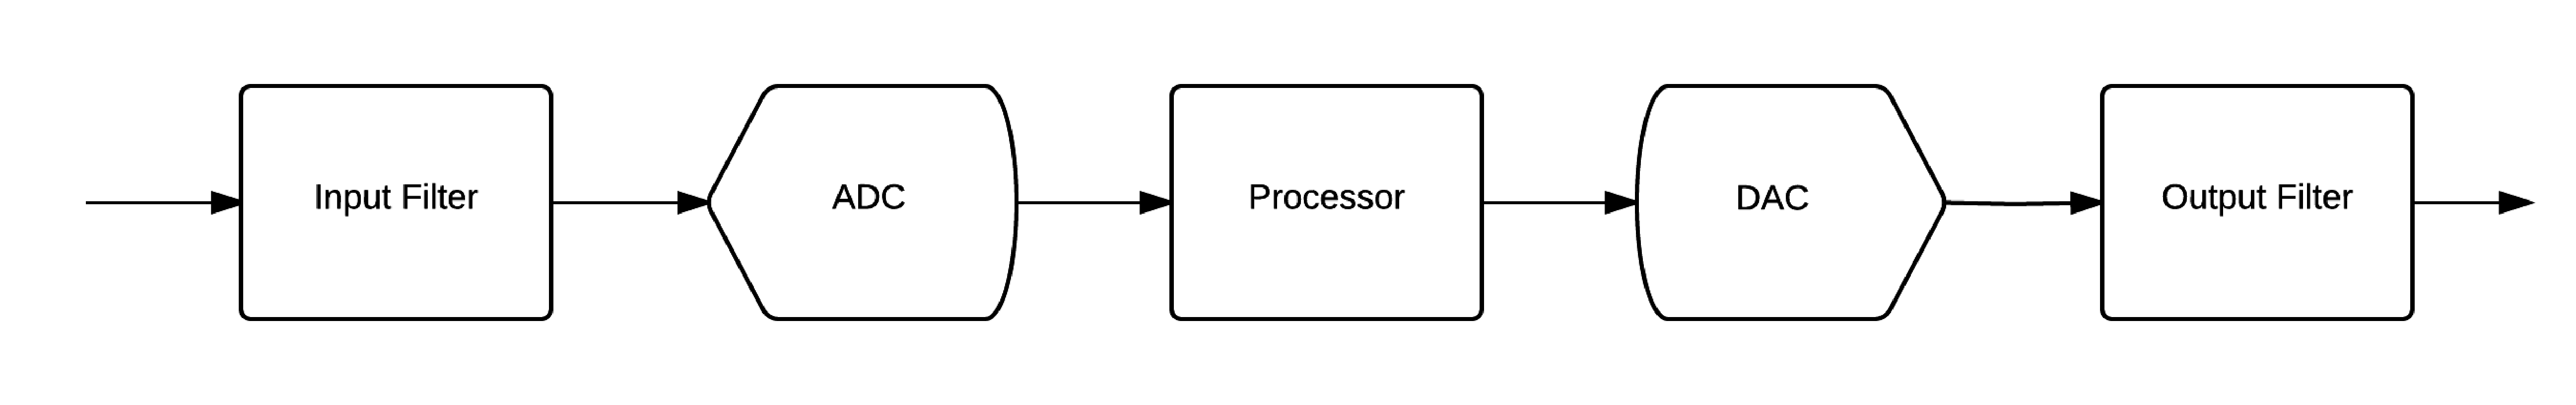
\includegraphics[width=0.8\textwidth]{./figures/sdr_basic_arch}
    \caption{ Software Defined Radio Basic Architecture
    \label{fig:sdr_basic}}
\end{figure}


Implementations may vary a lot, some common implementations are Made in matlab
through Simulink and use the computer’s video card as a medium of communication.
A more difficult but more interesting implementation involves the use of DSP
chips to implement the signal processing functions and some cheap ADC and DAC
chips can compose the SDR system.\\

The most commercial and famous implementation of SDR is Gnuradio+USRP, USRP
stands for Universal Software Radio Peripheral \cite{web:usrp} and Gnuradio
\cite{web:gnuradio} is a software for PC which has various digital signal
processing functions and modulation schemes and comes with a driver to use USRP.
The USRP itself is basically and FPGA hooked with a transceiver, so this pair is
broadly used in research and academic environments.\\

When we talk about research and development of real-world systems there is
always a tradeoff or bottleneck, in SDR the bottleneck is the hardware related
to the antenna interface, the antenna is designed to work better in a specific
bandwidth, this can limit the application, of course this is only one example of
bottleneck, there are others like Oscillator frequency, PLL, and processor
capability.\\

This work has a SDR like implementation done in FPGA and using the transceiver
AD9361 which makes baseband upconversion (Transmitter) and downconversion
(Receiver), filters and make analog to digital conversion and digital to analog
conversion, thus it is possible to implement transmitter and receiver with only
one board, however the most complex part does not lie in the system itself
because some electronic parts became a commodity, the complexity is in the
modulation/demodulation blocks and all the synchronization process, such topics
shall be discussed in the chapter \ref{cap:digitalcomm}.

\chapter{Long Term Evolution}
\label{chap:lte}

\section{Digital Communications Overview}
\label{lte:digicomm}

The purpose of a digital communication system is to transport an information
bearing signal from a source to a user destination via a communication channel.
The transmitter, receiver and channel are the three basic elements of a digital
communication system as shown in Figure \ref{fig:digicomsimple}. The message
produced by a source is a digital message, binary and not electrical. An input
transducer is used for converting the message to a time-varying electrical
quantity called waveform. Similarly, at the destination point, another transducer
converts the electrical waveform to the appropriate message.


%esquema básico do sistema de comunicacao
\begin{figure}[htbp]
    \centering
    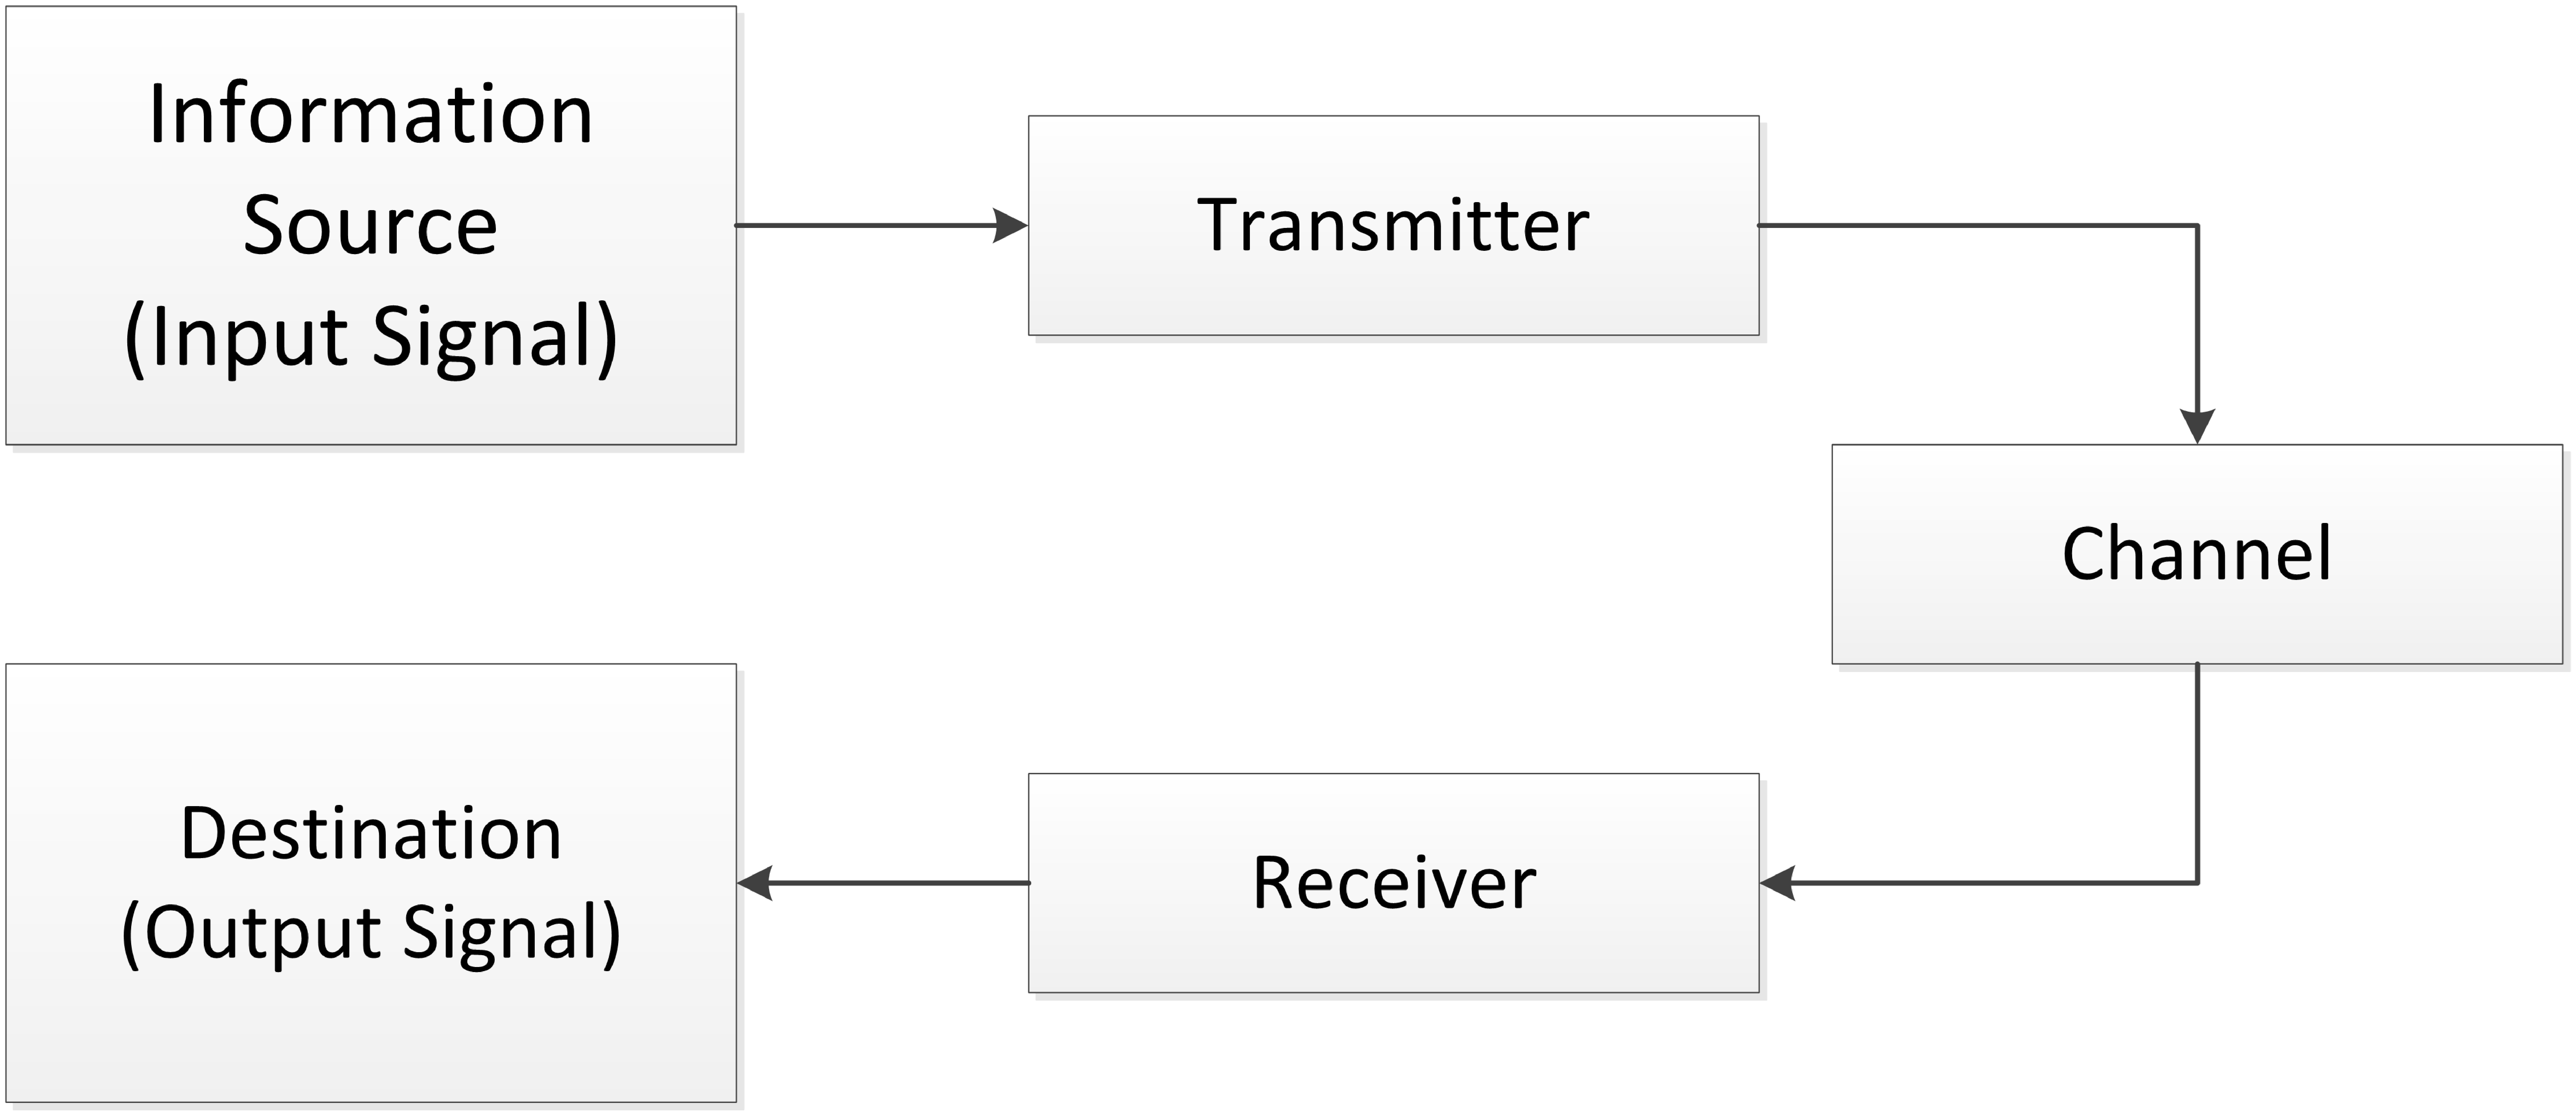
\includegraphics[width=0.65\textwidth]{./figures/digicom_simple}
    \caption{ A simple digital communication system block diagram.
    \label{fig:digicomsimple}}
\end{figure}

The transmitter is located at one point in space, the receiver is located at
some other point separate from the transmitter, and the channel is the medium
that provides the electrical connection between them. The former (transmitter),
in particular, is designed aiming to produce waveforms suitable for transmission
over the channel, a waveform. In the receiver the signal is normally corrupted
version of the transmitted signal, which is due to channel imperfections, noise
and interference. The receiver is designed to reconstruct a recognizable form of
the original message signal and to deliver it to a destination.

\subsection{Elements of Digital Communications Systems}

%block diagram of a digital communication system
\begin{figure}[htbp]
    \centering
    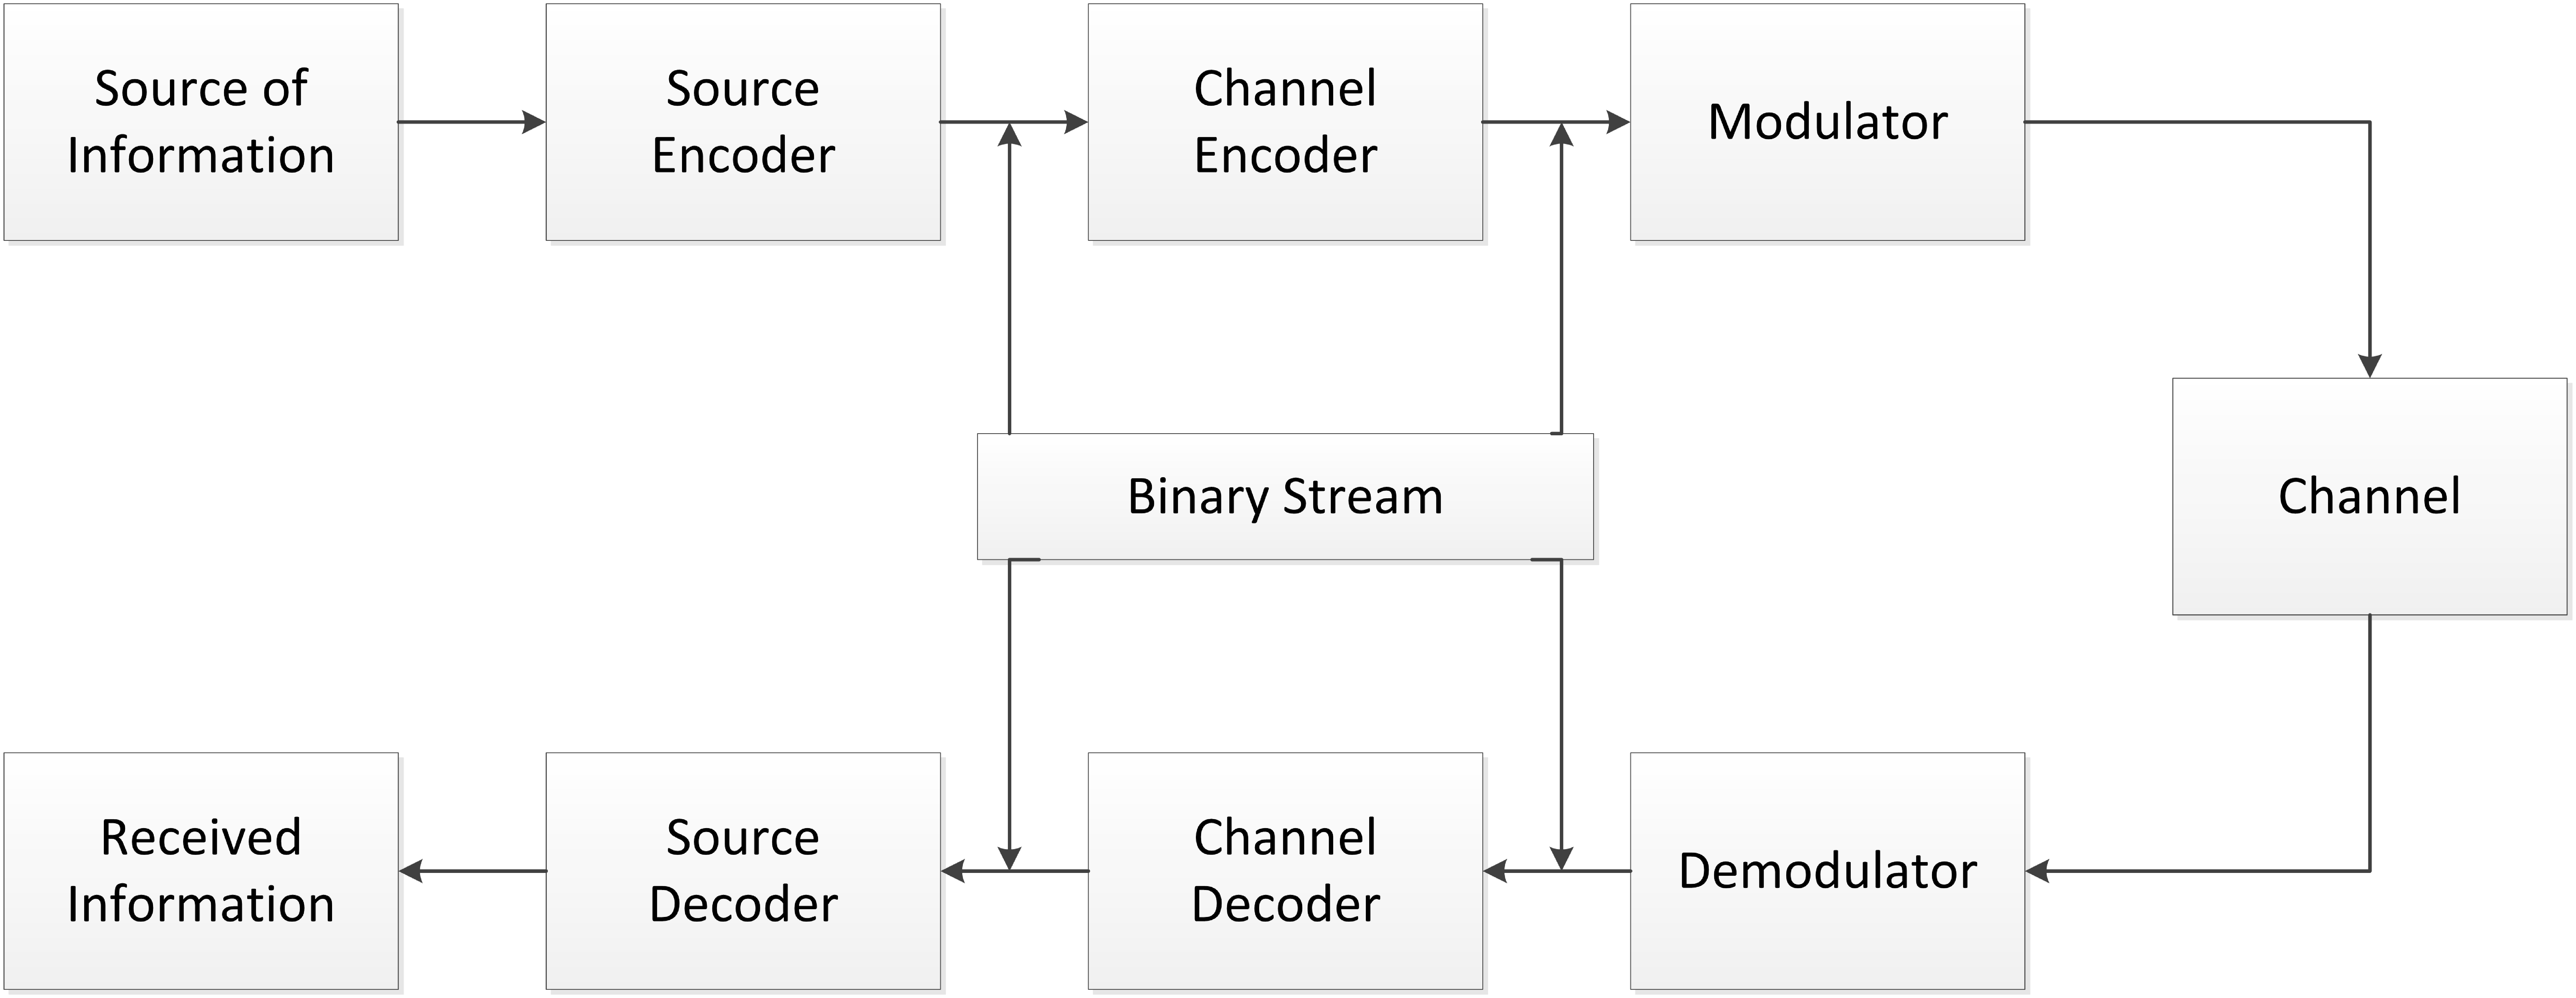
\includegraphics[width=0.85\textwidth]{./figures/digicom_bd}
    \caption{ Digital communication system block diagram.
    \label{fig:digcombd}}
\end{figure}

\subsubsection{Source of information}

The sources of information can be of two main kinds, \emph{analog information
sources} and \emph{digital information sources}. Analog information sources can
be human like voice, or natural like a humming bird. However, since Digital
communication systems work with a discrete and finite alphabet of symbols such
signals have to be converted to digital information prior to any process. Any
device that can record images or voice from the real world and can reproduce
back is making such analog to digital an digital to analog conversions
respectively.

Digital information sources are basically any information that was not
recorded or generated in the real world, it was generated by a software in a
PC. For example a digital painting or a 3D model.

\subsubsection{Source Encoder / Decoder}

The \emph{source encoder}  and \emph{source coder} converts the input symbol
sequence into a binary sequence (0 and 1) by assigning codewords to the symbols
in the input sequence. Basically the source encoder input is a analog waveform
and it samples, quantize and compress this analog waveform to a binary message
\cite{ocw:digicomm}.

At the receiver, the \emph{source decoder} converts the binary output of the
channel decoder into a analog waveform, doing the opposite operations of the
\emph{source encoder}. The decoder for a system using fixed length code words is
quite simple, but the decoder for a system using variable length code words can
be very complex \cite{ocw:digicomm}.

Aim of the source coding is to remove the redundancy in the transmitting
information, so that bandwidth required for transmission is minimized. This
approach is based on the probability of the symbol codeword is assigned. The
higher the probability, the shorter the codeword.

\subsubsection{Channel Encoder / Decoder}

Error control is accomplished by the channel coding operation that consists of
systematical addition of extra bits to the output of the source coder. These
extra bits do not convey any information but helps the receiver to detect and/or
correct some of the errors in the information bearing bits. There are two
methods of channel coding, the \textit{Block Coding} and \textit{Convolution
Coding}.

In the block coding method the encoder takes a block of ‘k’ information bits
from the source encoder and adds ‘r’ error control bits, where ‘r’ can be chosen
based on ‘k’ and error control capabilities desired, this process is
accomplished by a matrix multiplication and that is the origin of the "block" in
block coding. In the convolution coding process the message goes through a
sequence of tapped-delay line operations which works in the same way as
convolving the message with the impulse response of the code, with modulo-2
operations.

The Channel decoder recovers the information bits from the coded binary stream,
error detection and possible correction is also performed by the channel
decoder.

\subsubsection{Modulator}

The modulator converts the input bit stream into a waveform suitable for
transmission over the communication channel. Advanced modulation schemes such as
Orthogonal Frequency Division Multiplexing (OFDM) can be effectively used to
minimize the effects of channel noise to match the frequency spectrum of
transmitted signal with channel characteristics.

\subsubsection{Demodulator}

The extraction of the message from the information bearing waveform produced by
the modulation is accomplished by the demodulator. The output of the demodulator
are symbols which can be detected and the converted to bits to form a received
message.

\subsubsection{Channel}

The Channel is the medium of wave propagation (wireless in this work) then
creating a "connection" between transmitter and receiver. The different channels
are: pair of wires, coaxial cable, optical fiber, radio channel, satellite
channel or combination of any of these.

\subsection{Additional Modules}

%augmented block diagram
\begin{figure}[htbp]
    \centering
    
\includegraphics[width=0.85\textwidth]{./figures/digicom_plus}
    \caption{ Digital communication system block diagram with additional blocks.
    \label{fig:digicomplus}}
\end{figure}

Some additional blocks as shown in the block diagram  at Figure \ref{fig:digicomplus}
are used in most of digital communication system:

\begin{itemize}

  %\item \textbf{Encryptor:} Encryptor prevents unauthorized users from
    %understanding the messages and from injecting false messages into the system.

  \item \textbf{Multiplexer:} Multiplexer is used for combining signals from
different sources so that they share a portion of the communication system.

  \item \textbf{Demultiplexer:} DeMultiplexer is used for separating the different
signals so that they reach their respective destinations.

  %\item \textbf{Decryptor:} It does the reverse operation of that of the Encryptor.

\end{itemize}

\subsection{Synchronization}

Synchronization involves the estimation of both time and frequency. Coherent
systems need to synchronize their frequency reference with carrier in both
frequency and phase (carrier recovery). The synchronization begins with the
Automatic Gain Control (AGC) which scales the received waveform to a know power
level, then the timing recovery or carrier recovery process can be executed.

Timing or symbol recovery is the process of by with the receiver estimates the
symbol frequency of the received waveform, that process results in the best time
instants to sample a received waveform. Timing recovery is a requirement of all
digital communication systems \cite{akbook}.

Carrier recovery is a processes used in both coherent and non-coherent
demodulation where the phase and the frequency of the transmitter carrier wave
are recovered by the receiver and thus after having such information it is
possible to extract the information in the transmitted signal. Considering that
the phase and frequency of the transmitted wave probably will be affected by
noise, it is not a straight-forward method, it includes filtering and usually
feedback systems (PLLs) to correct the errors in phase or frequency caused by
the noise.

%-----------------------------------LTE-----------------------------------------

\section{Long Term Evolution} %OK
\label{let:lte}

\subsection{Overview}

Long Term Evolution (LTE) is a standard for wireless communication for
high-speed mobile devices and data terminals. LTE was first introduced in 3GPP
Release 8. It uses orthogonal frequency division multiplexing (OFDM) as its
radio access technology, together with advanced antenna technologies.

In addition to LTE, 3GPP also defined an IP-based, flat core network
architecture. This architecture was defined as part of the System Architecture
Evolution (SAE) effort specifying the Evolved Packet Core (EPC) network. The
LTE-SAE architecture and concepts have been designed for efficient support of
mass-market usage of any IP-based service. The architecture is based on an
evolution of the existing GSM/WCDMA core network.%, with simplified operations
%and smooth, cost-efficient deployment.

Moreover, work has also been done by 3GPP in cooperation with 3GPP2 (the CDMA
standardization body) to optimize interworking between CDMA and LTE-SAE. This means
that both CDMA and GSM operators can use the same standard with minor modifications
and thus making the deployment and roaming costs smaller.

The 3GPP radio access technology was developed towards and reduce cost per bit
implicating a lower cost and more variated services with a better user
experience. It was also thought in the flexibility of the existing and new
frequency  bands, giving LTE an scalable bandwidth (20MHz, 15MHz, 10MHz, 5MHz,
3MHz and 1.4MHz). Another noteworthy point is that the architecture and open
interfaces are simplified.

\subsection{Orthogonal Frequency-division Multiplexing Radio Technology} %+/-ok

LTE uses OFDM for the downlink (from the base station to the terminal or UE).
OFDM meets the LTE requirement for spectrum flexibility and enables
cost-efficient solutions for very wide carriers with high peak rates. It is a
well-established modulation scheme: for example, adopted in standards IEEE
802.11a/b/g, 802.16, HIPERLAN-2, DVB and DAB.

A representation of an OFDM signal can be seen in Figure \ref{fig:ofdmfreq}. In
this figure, a signal with 5 MHz bandwidth is shown, but the principle is of
course the same for the other Evolved UMTS Terrestrial Radio Access (E-UTRA)
bandwidths. Data symbols are independently modulated and transmitted over a high
number of closely spaced orthogonal subcarriers.

%ofdm scheme
\begin{figure}[htbp]
    \centering
    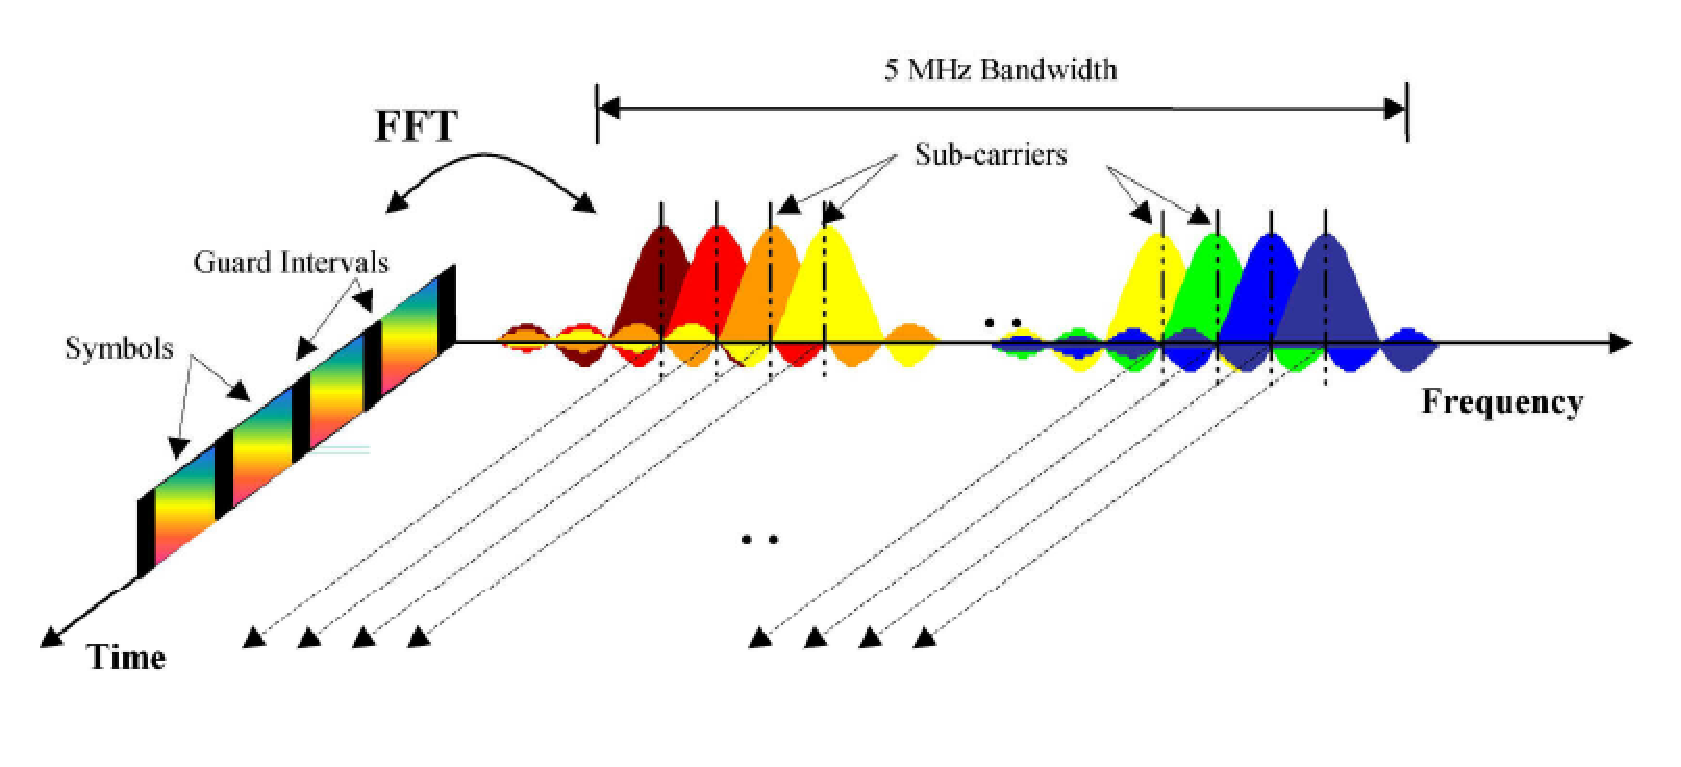
\includegraphics[width=0.65\textwidth]{./figures/ofdm_frequency}
    \caption{ Frequency-time representation of OFDM signal.
    \label{fig:ofdmfreq}}
\end{figure}

OFDM uses a large number of sub-carriers for multi-carrier transmission. The
basic LTE downlink physical resource can be seen as a time-frequency grid. In
the frequency domain, the spacing between the sub-carriers is 15 kHz. In
addition, the OFDM symbol duration time is $\frac{1}{\Delta f} + \text{cyclic
prefix duration}$. The cyclic prefix is used to maintain orthogonality between
the sub-carriers even for a time-dispersive radio channel.

The OFDM symbols are grouped into resource blocks. The resource blocks have a
total size of 180 kHz in the frequency domain and 0.5ms in the time domain. Each
user is allocated a number of so-called resource blocks in the time-frequency
grid and inside a resource block there are 12 subcarriers. The more resource
blocks a user gets, and the higher the modulation used in the resource element,
the higher the bit rate. Which resource blocks the user gets at a given point in
time, and how many, depends on advanced scheduling mechanisms in the frequency
and time dimensions. One resource element carries QPSK, 16QAM or 64QAM. With
64QAM, each resource element carries six bits.

In the uplink, LTE uses a pre-coded version of OFDM called single carrier
frequency division multiple access (SC-FDMA). This is to compensate for a
drawback with normal OFDM, which has a very high peak to average power ratio
(PAPR). High PAPR requires expensive and inefficient power amplifiers with high
linearity requirements, which increases the cost of the terminal and drains the
battery faster \cite{introlte}, \cite{umtslte}.

SC-FDMA solves this problem by grouping together the resource blocks in such a
way that it reduces the PAPR. Thus, it avoids the need for wider linear
operation bands of the power amplifier and also power consumption. A low PAPR
also improves coverage and cell-edge performance \cite{introlte}.

Since this work shall focus on the radio frontend part of the system, implementing
a downlink scheme, it is interesting to dwell more in the LTE downlink and uplink
schemes.

\subsection{Downlink Scheme}%OK

The downlink transmission scheme for E-UTRA FDD and TDD modes is based on
conventional OFDM. In an OFDM system, the available spectrum is divided into
multiple carriers, called subcarriers as explained in the previous subsection.
Each of these subcarriers is independently modulated by a a low rate data
stream, which allows robustness against multipath fading and efficient
equalization schemes.

The user data is carried on the Physical Downlink Shared Channel (PDSCH). The
PDSCH is the only channel that can be QPSK, 16QAM or 64QAM modulated. The
Downlink channel schematic can be seen in Figure \ref{fig:dlchann} with channels
delay spread. The delay spread is the time between the symbol arriving on the
first multi-path signal and the last multi-path signal component, typically
several $\mu s$ dependent on the environment (i.e. indoor, rural, suburban, city
center). The guard interval has to be selected in that way, that it is greater
than the maximum expected delay spread. In E-UTRA, the guard interval is a
cyclic prefix which is inserted prior to each OFDM symbol.

In practice, the OFDM signal can be generated using \textit{IFFT} (Inverse Fast
Fourier Transform) operation. The \textit{IFFT} converts a number N of complex
data symbols used in the frequency domain bins into the time domain signal. Such
an N-point \textit{IFFT} is illustrated in Figure \ref{fig:ofdmsymbol} where
$a(mN+n)$ refers to the nth subcarrier modulated data symbol, during the time
period $mT_u < t \le (m+1)T_u$ \cite{umtslte}.

%ofdm symbols
\begin{figure}[htbp]
    \centering
    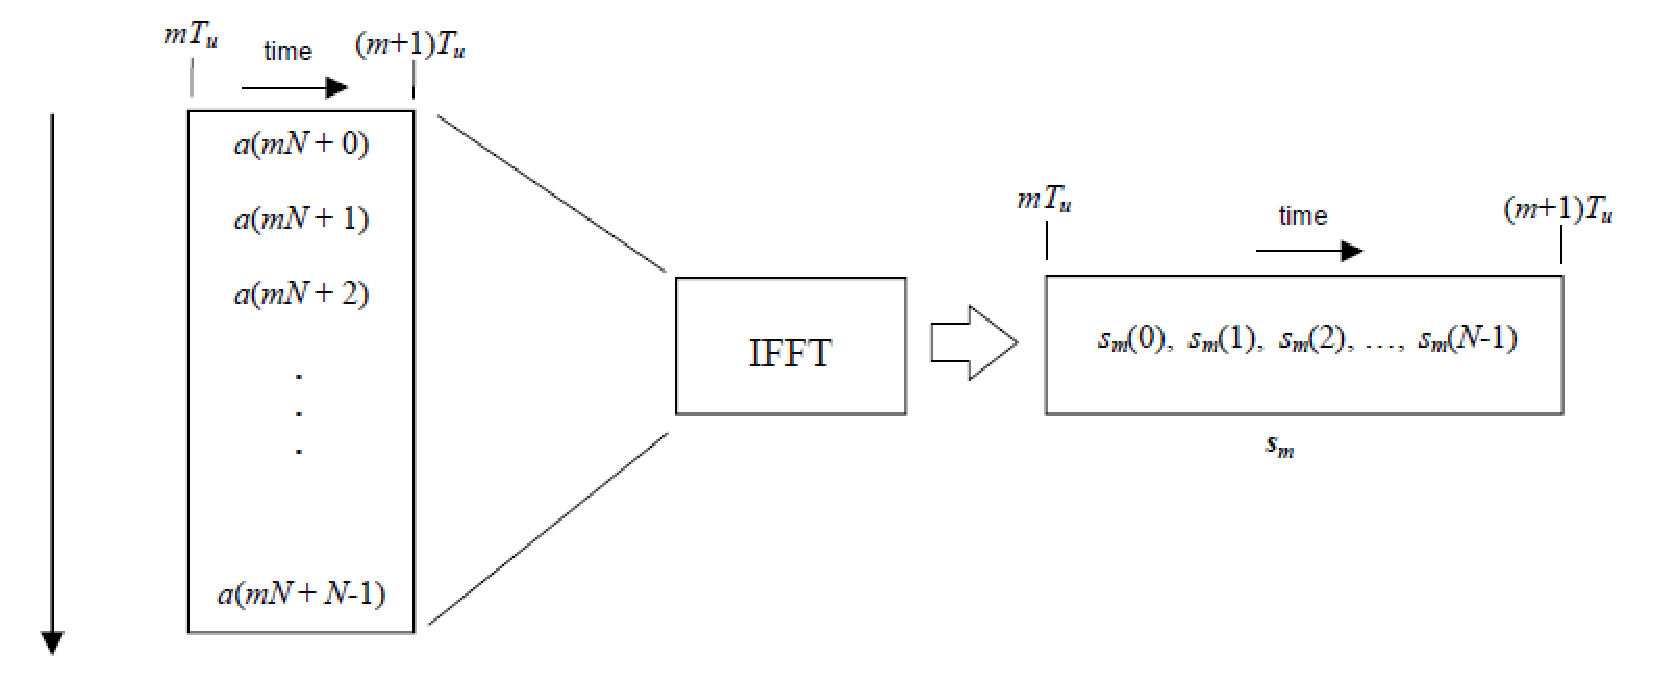
\includegraphics[width=0.65\textwidth]{./figures/ofdm_symbol_gen}
    \caption{ OFDM symbol generation \cite{umtslte}.
    \label{fig:ofdmsymbol}}
\end{figure}

The vector $sm$ is defined as the \emph{time-domain OFDM symbol}. It is the time
superposition of the $N$ narrowband modulated sub-carriers. Therefore, from a
parallel stream of $N$ sources of data, each one independently modulated, a
waveform composed of N orthogonal sub-carriers is obtained. Figure
\ref{fig:ofdmchain} illustrates the mapping from a serial stream of QAM symbols
to N parallel streams, used as frequency domain bins for the \textit{IFFT}. The
N-point time domain blocks obtained from the \textit{IFFT} are then serialized
to create a time domain signal.

%ofdm signal chain
\begin{figure}[htbp]
    \centering
    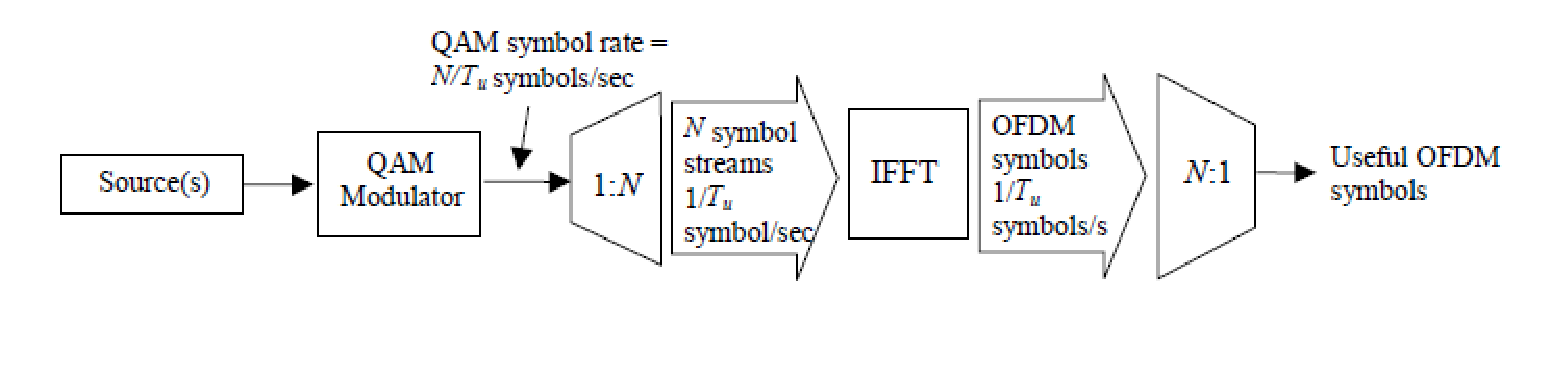
\includegraphics[width=0.65\textwidth]{./figures/ofdm_signal_chain}
    \caption{ OFDM signal generation \cite{umtslte}.
    \label{fig:ofdmchain}}
\end{figure}

In contrast to an OFDM transmission scheme, \textit{OFDM}A allows the access of
multiple users on the available bandwidth. Each user is assigned a specific
time-frequency resource. The data is allocated to a device (User Equipment, UE)
in terms of resource blocks, this means that one UE can be allocated integer
multiples of one resource block, whose representation can be seen in Figure
\ref{fig:ofdmresblk}. These resource blocks do not have to be adjacent to each
other. In the time domain, the scheduling decision can be modified every
transmission time interval of 1 ms corresponding to LTE sub-frame. All scheduling
decisions for downlink and uplink are done in the base station (enhanced NodeB,
eNodeB or eNB). The scheduling algorithm has to take into account the radio link
quality situation of different users, the overall interference situation,
Quality of Service requirements, service priorities, etc. and is a
vendor-specific implementation.

%ofdm resource block
\begin{figure}[htbp]
    \centering
    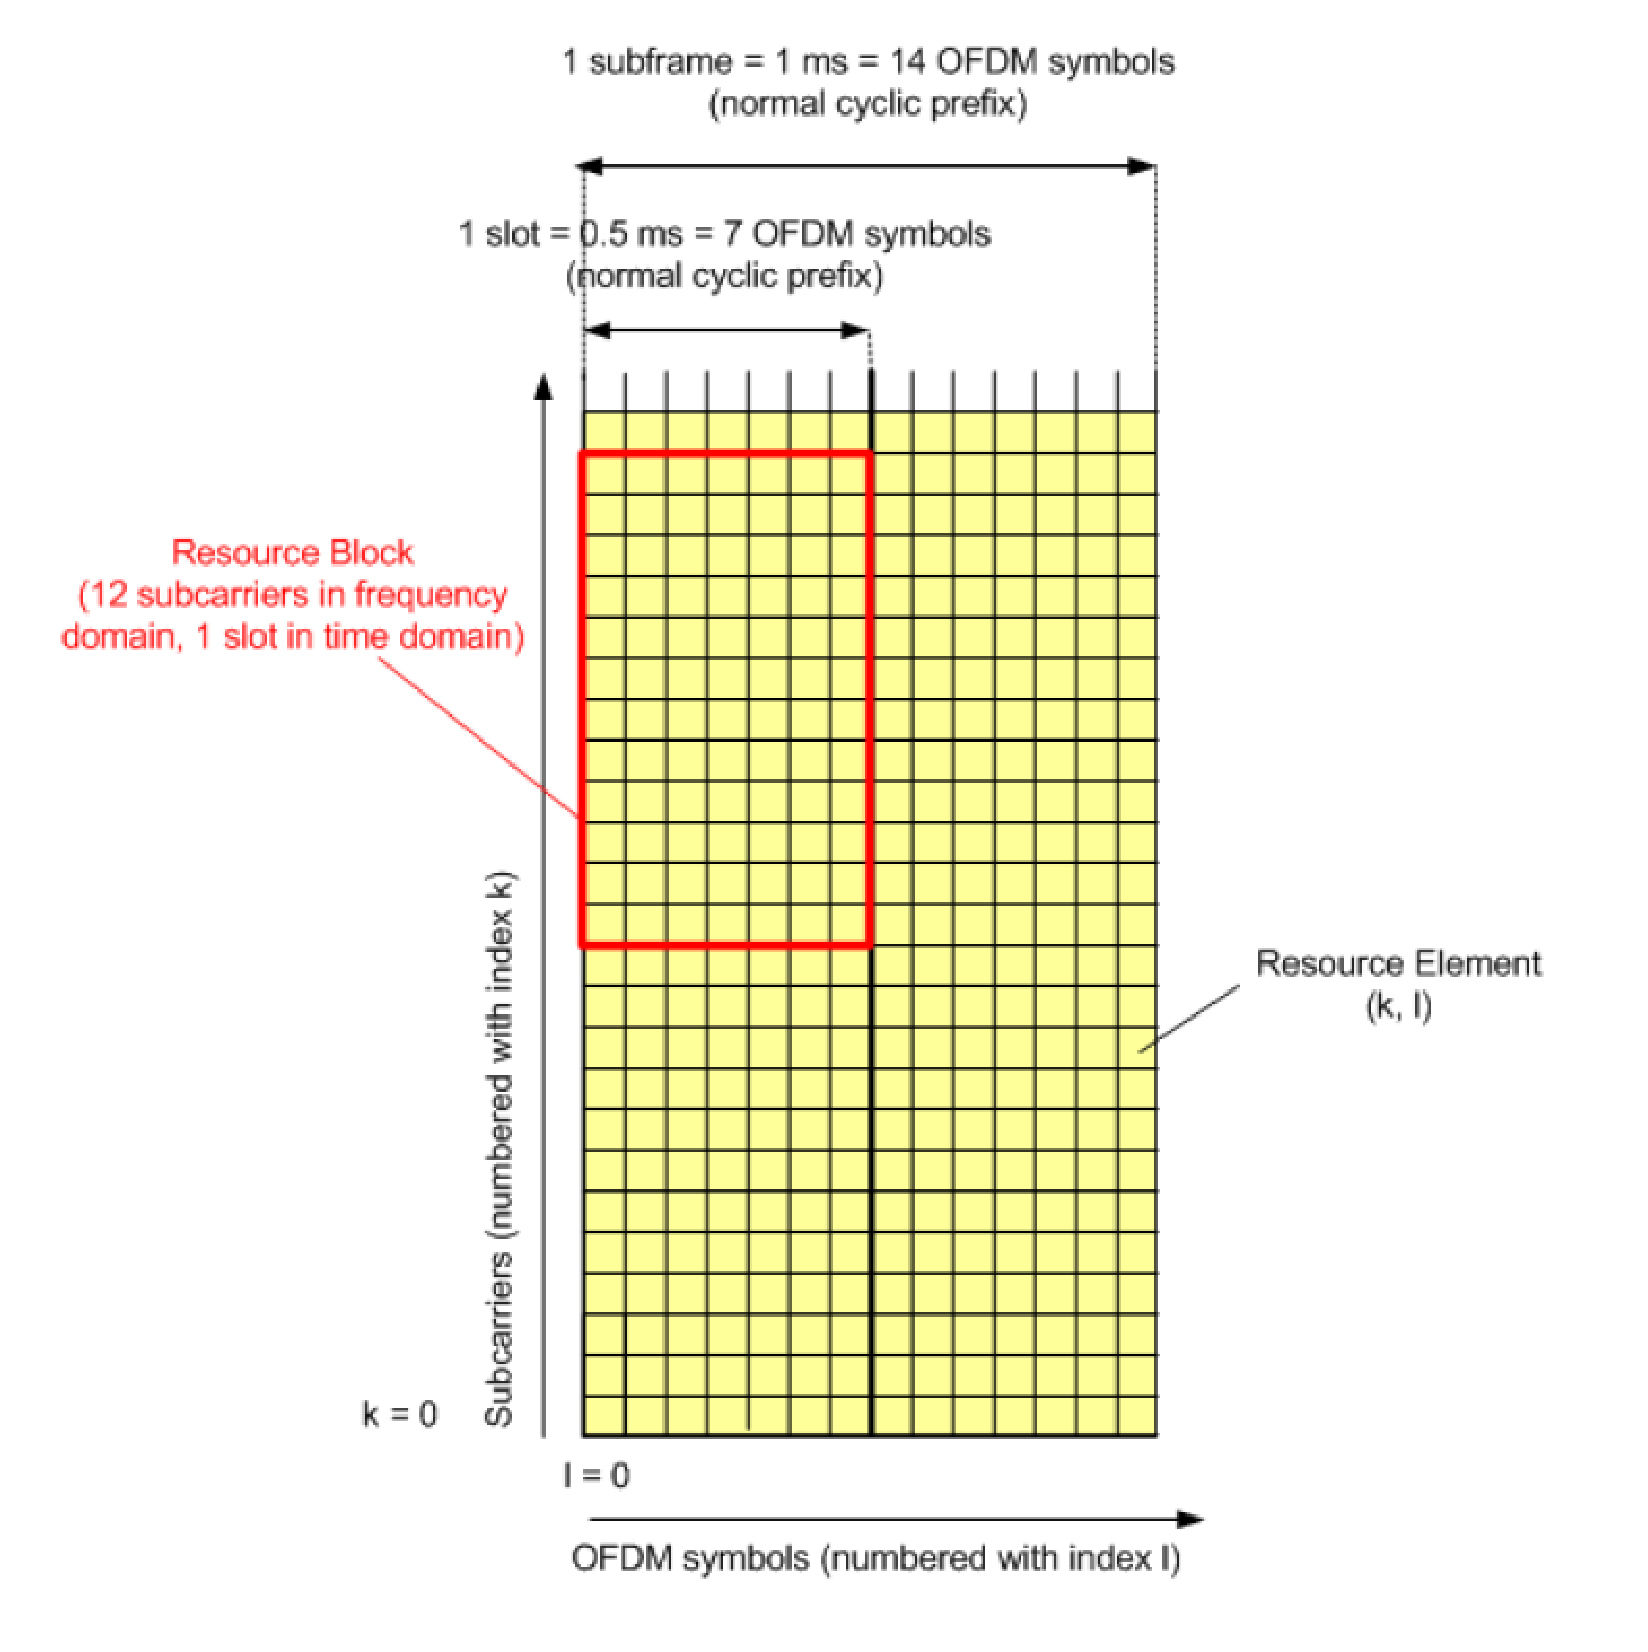
\includegraphics[width=0.65\textwidth]{./figures/ofdm_resource_block}
    \caption{ Resource block organization example \cite{umtslte}.
    \label{fig:ofdmresblk}}
\end{figure}

%downlink channel figura
\begin{figure}[htbp]
    \centering
    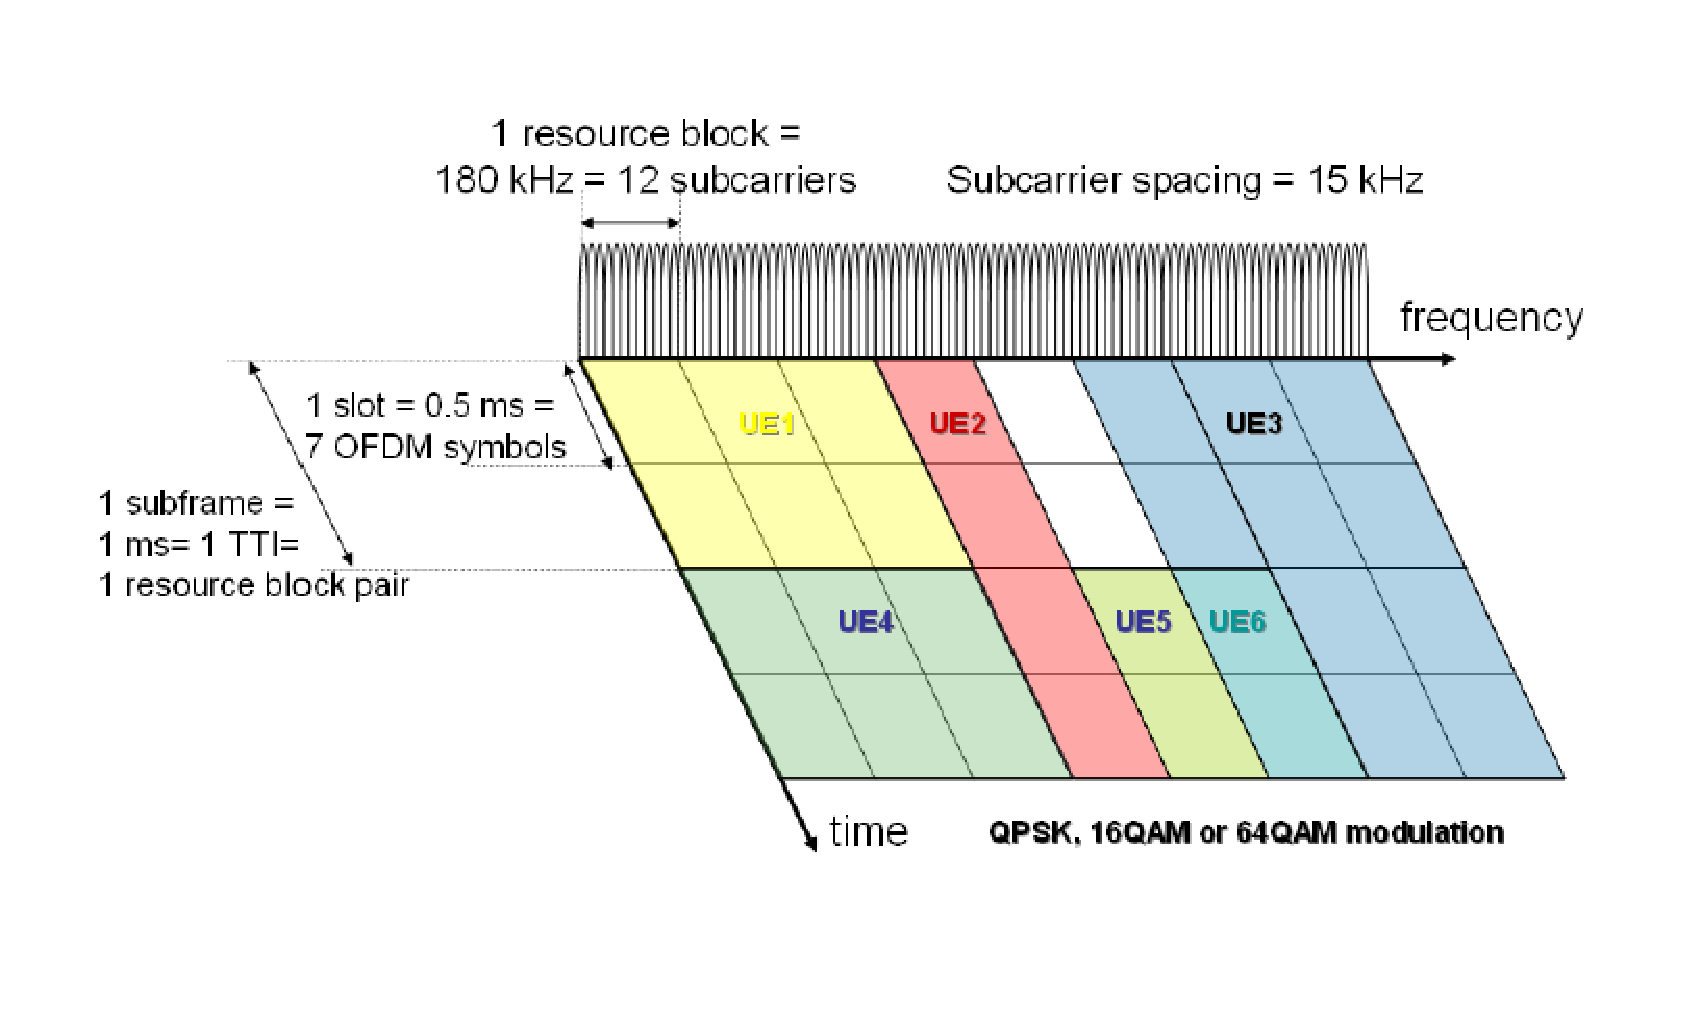
\includegraphics[width=0.70\textwidth]{./figures/downlink_channels}
    \caption{ OFDMA time-frequency multiplexing.
    \label{fig:dlchann}}
\end{figure}


\subsection{Uplink Scheme}%ok

During the study item phase of LTE, alternatives for the optimum uplink
transmission scheme were investigated \cite{umtslte}. While \textit{OFDMA} is
seen optimum to fulfill the LTE requirements in downlink, \textit{OFDMA}
properties are less favorable for the uplink. This is mainly due to unfavorable
PAPR properties of an \textit{OFDMA} signal, resulting in worse uplink coverage
and challenges in power amplifier design for battery operated handset, as it
requires expensive power amplifiers.

Thus, the LTE uplink transmission scheme for FDD and TDD mode is based on SC-
FDMA with cyclic prefix. Still, SC-FDMA signal processing has some similarities
with \textit{OFDMA} signal processing, so parameterization of downlink and
uplink can be harmonized.

There are different possibilities for generating an SC-FDMA signal. DFT-spread-
\textit{OFDM} \textit{(DFT-s-OFDM)} has been selected for E-UTRA. For
DFT-s-OFDM, a size-M DFT is first applied to a block of M modulation symbols,
prior to the IFFT. Then, QPSK, 16QAM and 64QAM are used as uplink E-UTRA
modulation schemes, the latter being optional for the UE. The DFT transforms the
modulation symbols into the frequency domain. The result is mapped onto the
available number of subcarriers. For LTE Release 8 uplink, only localized
transmission on consecutive subcarriers is allowed. An N-point \textit{IFFT}
where $N>M$ is then performed as in OFDM, followed by addition of the cyclic
prefix and parallel to serial conversion. The complete uplink scheme can be
illustrated by the diagram in Figure \ref{fig:uplinkbd}.

%figura uplink
\begin{figure}[htbp]
    \centering
    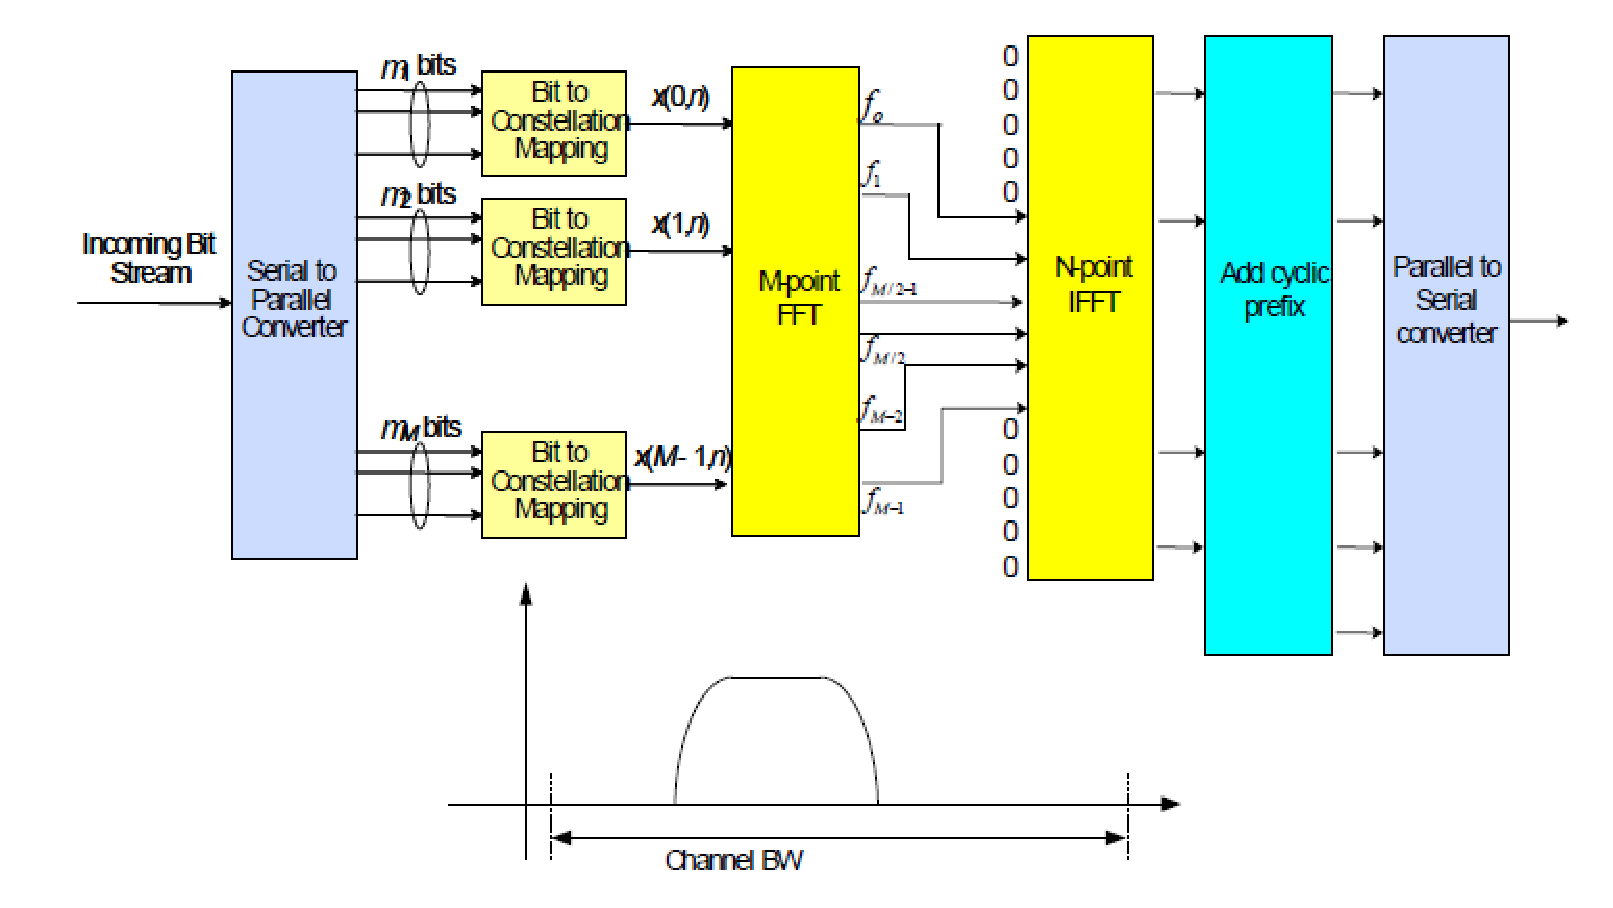
\includegraphics[width=0.65\textwidth]{./figures/uplink_scheme}
    \caption{ LTE uplink block diagram of DFT-s-OFDM.
    \label{fig:uplinkbd}}
\end{figure}


\part{Implementation}
\chapter{Setup Implementation}

\section{Overview}

\section{FPGA}

\subsection{ML605 - Virtex6}
\subsection{VC707 - Virtex7}

\section{Transceiver - FMComms2}
\subsection{AD9361}
\label{sec:ad9361}

The AD9361 is a high performance RF transceiver. Its programmability and adaptability makes it ideal for a wide range of transceiver applications. This device combines a RF front end with a flexible and configurable mixed-signal baseband section and frequency synthesizers, simplified configuration digital interface to a processor.
The AD9361 operates from 70 MHz to 6.0GHz range with supported channel bandwidths from 200 KHz to 56 MHz and the AD9361 is a 2 Rx and 2 Tx device packed in a 10mm x10mm, 144 ball chip package ball grid array (CSP\_BGA).

\subsubsection{General Description}

AD9361 is a highly integrated RF frequency transceiver capable of being configured for a wide range of applications, including 3g and 4g frequency applications. AD9361 and AD9364 almost the same hardware and specifications, the difference is that AD9361 is a 2x2 MIMO and AD9364 is a 1x1 \cite{ad9361_wiki}.
The programmability allows the AD9361 to be operated in Frequency Division Duplex (FDD) and Time Division Duplex (TDD) systems, allowing this transceiver to operate in a variety of communication standards. Another interesting feature is the capability of integration with a wide range of BBPs (Baseband Processors) using a single or dual 12-bit parallel data port or a 12-bit LVDS (Low voltage Differential signaling), which uses the FMC connector in the FMCommS2 \ref{sec:fmcomms2}.
AD9361 also provides self-calibration and automatic gain control (AGC) systems to maintain good performance under variable conditions, such as temperature and signal quality. The transceiver has also various modes of test mode with the Built-in Self Test (BIST) modes which can be used for the designers to debug desgs during prototyping.
This configurability and adaptability is very attractive for Software Defined Radio (SDR) and for C-RAN systems, indeed ad9361 is already being used in some Universal Software Radio Peripheral (USRP) from ettus research (National Instruments), this alone is a proof that AD9361 can work in a wide range of systems and standards.

\begin{figure}[htbp]
    \centering
    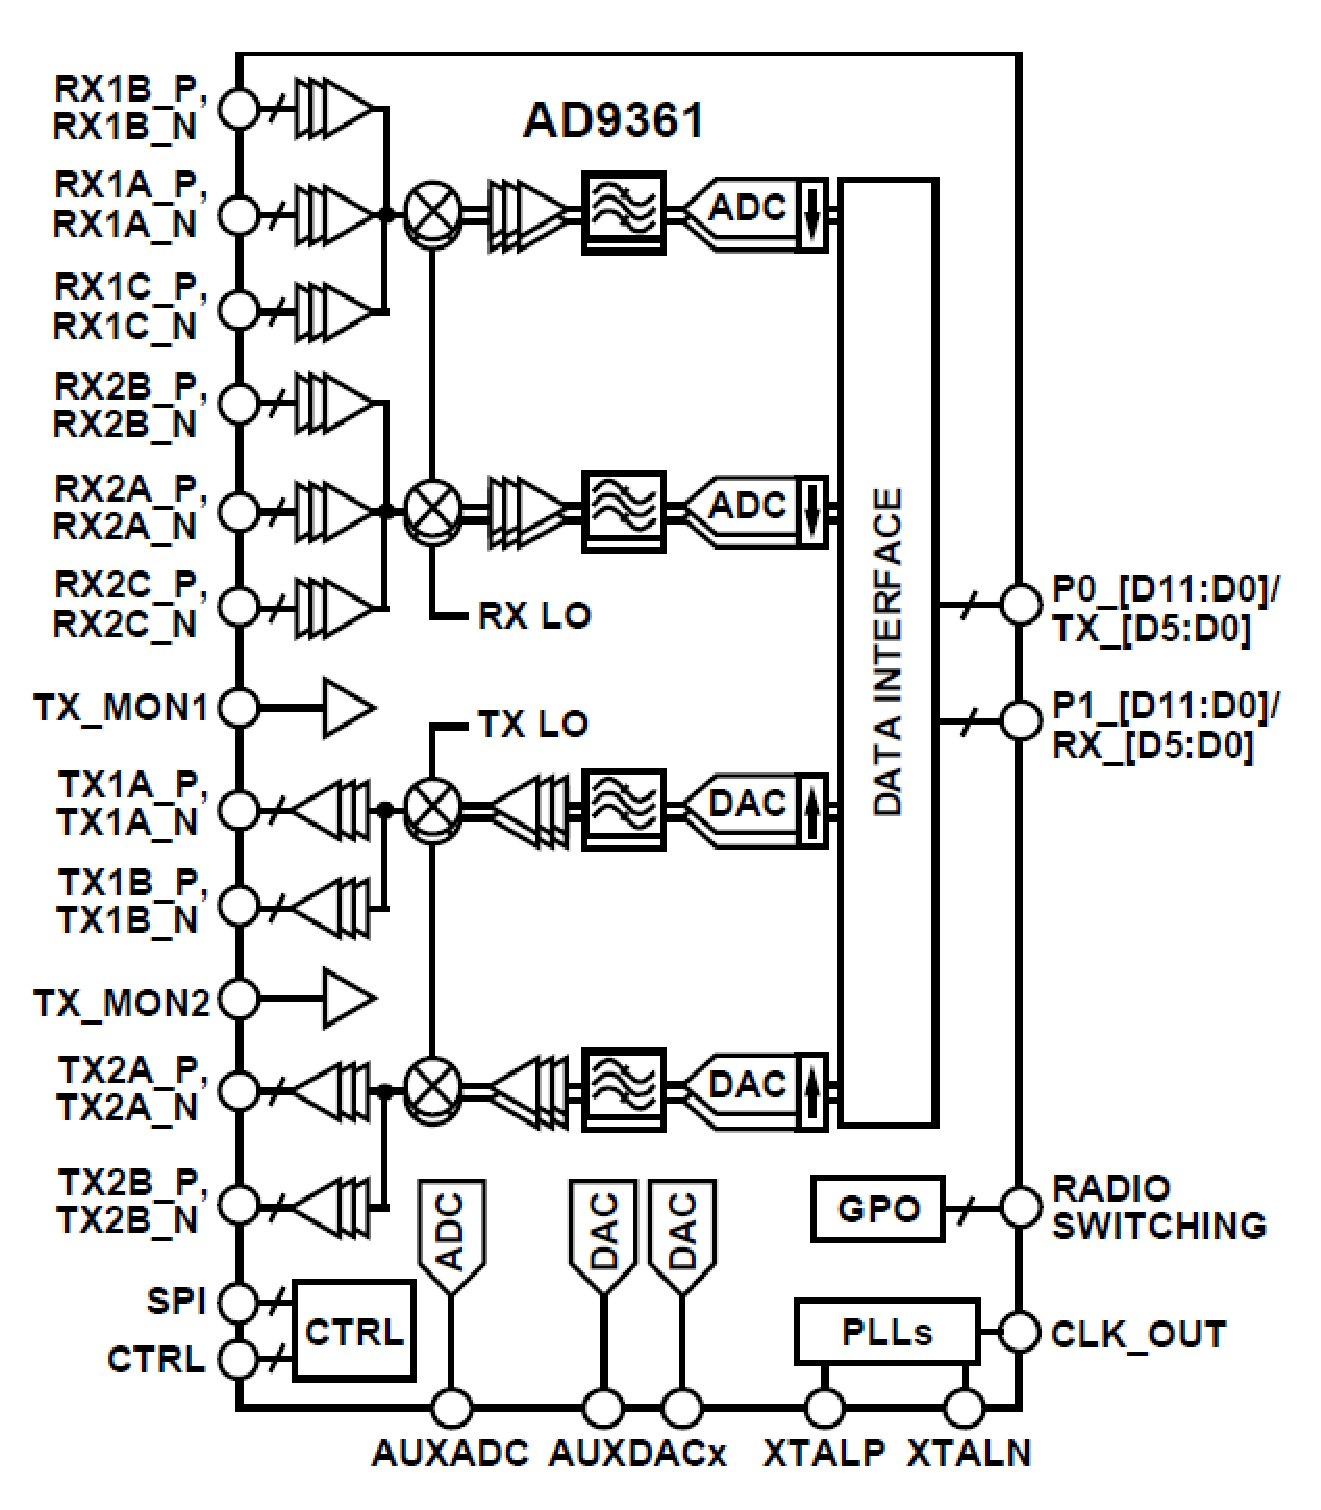
\includegraphics[width=0.65\textwidth]{./figures/ad9361_functional_diagram}
    \caption{ AD9361 Functional Block Diagram
    \label{fig:ad9361func}}
\end{figure}

\subsubsection{Receiver}

The receiver section has all the blocks necessary to receive analog RF signals and convert them to digital data which can be used by the BBP. there are two independently controlled channels that share same frequency synthesizer. This characteristic makes possible to the AD9361 to operate in MIMO systems.

Each channel has 3 inputs which can be multiplexed into the signal chain, making possible to use the AD9361 into systems with multiple antenna inputs. The Receiver is a direct conversion system that contains a Low noise amplifier (LNA) , followed by a matched in-phase and quadrature amplifier, mixers, and band shaping filters that down convert received signals to baseband for digitization. External LNAs can also be interfaced to the AD9361 allowing more flexibility in the design.
The receiver signal path passes downconverted signals (I and Q), which are schematically identical to each other,  to the baseband (BB) receiver section. The BB section is composed by two programmable low-pass filters, with programmable corner frequency for each filter, 12-bit ADC and four stages of decimating filters, each of the four decimation filters can be bypassed.
The gain control is achieved by a preprogrammed gain index map, a lookup table for example, this map distributes gain in order to achieve optimal performance at each level. This optimal behavior can be achieved by enabling AGC, which can run in two modes, fast and slow gain control. This allow for the BBP to make gain adjustments as needed.
Each channel also contains independent RSSI measurement capability, DC offset tracking and all other circuitry needed for self-calibration.

The receiver ADC is a 12-bit sigma-delta ($\Sigma-\Delta$) ADC which allows adjustable sample rates. This ADC produces data streams from the received signals and such digitalized signals can be conditioned further by a series of decimation filters and a 128-tap FIR filter with additional decimation settings.
The sampling rate of each digital filter is adjustable through changes in the decimation factors to produce the needed data rate.

In short, the Receiver chain has:

\begin{itemize}
	\item LNA - Low noise Amplifier
	\item Matched in-phase amplifier;
	\item Quadrature Amplifier;
	\item Band Shaping Filters;
	\item Analog low pass filters;
	\item 12-bit DAC;
	\item 4 stages of decimation filters (128-tap FIR filters);
	\item Automatic gain Control;
\end{itemize}

\begin{figure}[htbp]
    \centering
    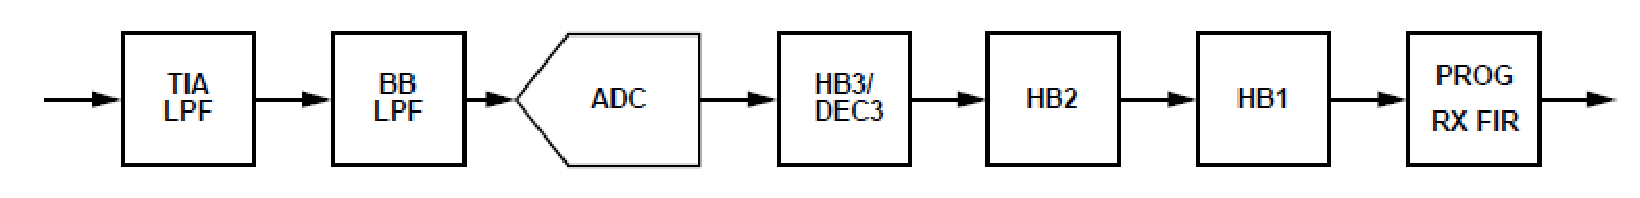
\includegraphics[width=0.65\textwidth]{./figures/rx_chain}
    \caption{ Receiver Signal Path
    \label{fig:rxchain}}
\end{figure}


\subsubsection{Transmitter}

Like the receiver section, the transmitter section contains two identical and independently controller channels, which share the same frequency synthesizer,  that provide all digital signal processing, mixed signal and RF blocks necessary to implement a direct conversion system from digital data to RF.
The Tx signal path receives from the BBP 12-bit 2s complement I-Q format data in the digital interface and each channel goes through a 128-tap FIR filter with interpolation options, which is fully programmable. Then the signal goes through a series of additional interpolation filters that manipulates the signal with additional filtering and data rate interpolation before reaching the 12-bit DAC, note that all these filtering and interpolation steps can be bypassed if desired.
Each 12-bit DAC has an adjustable sampling rate and its analog output passes through to low pass filters to remove any sampling artifacts before going to the RF mixer, these low pass filters corner frequencies can be programmable too. After all these filtering and analog conversion steps, the I and Q signals are recombined and modulated in the carrier frequency, which can be adjusted by changing the synthesizer frequency. These analog combined signals passes through additional analog filters for better band shaping and then it can be transmitted to the output amplifier. Each Transmitting channel provides wide attenuation adjustment range with fine granularity in order to optimize SNR.

\begin{figure}[htbp]
    \centering
    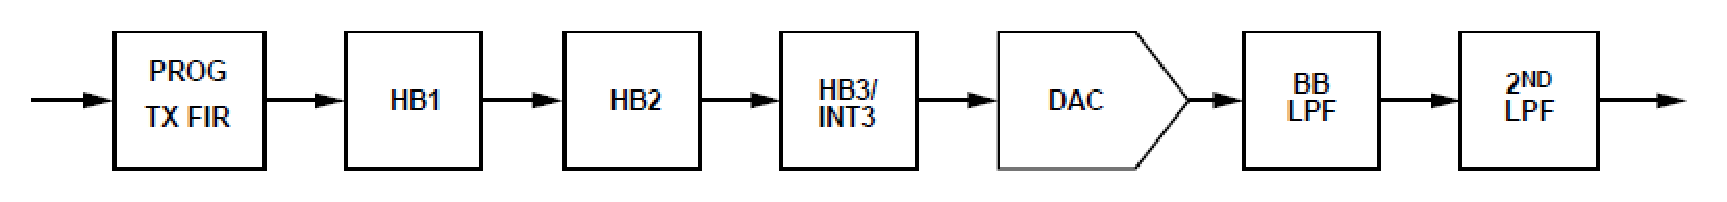
\includegraphics[width=0.65\textwidth]{./figures/tx_chain}
    \caption{ Transmitter Signal Path
    \label{fig:txchain}}
\end{figure}


Identical to the receiver chain, the transmitter chain has also built-in self-calibration circuitry into each transmitting channel providing an automatic real-time adjustment. The transmitter also provides a TX monitor block for each channel, this block monitors the transmission output and routes it back through an unused receiver channel to the BBP for signal monitoring, but these monitoring option is only available in TDD mode operation while the receiver is idle.

In short the transmission chain has:

\begin{itemize}
	\item 128-tap FIR filters;
	\item Interpolation Filters;
	\item 12-bit DAC;
	\item Analog Low-pass Filters;
	\item Additional band shaping analog filters;
	\item Attenuation adjustment;
	\item self-calibration circuits;
	\item Tx signal Monitor.
\end{itemize}

\begin{figure}[htbp]
    \centering
    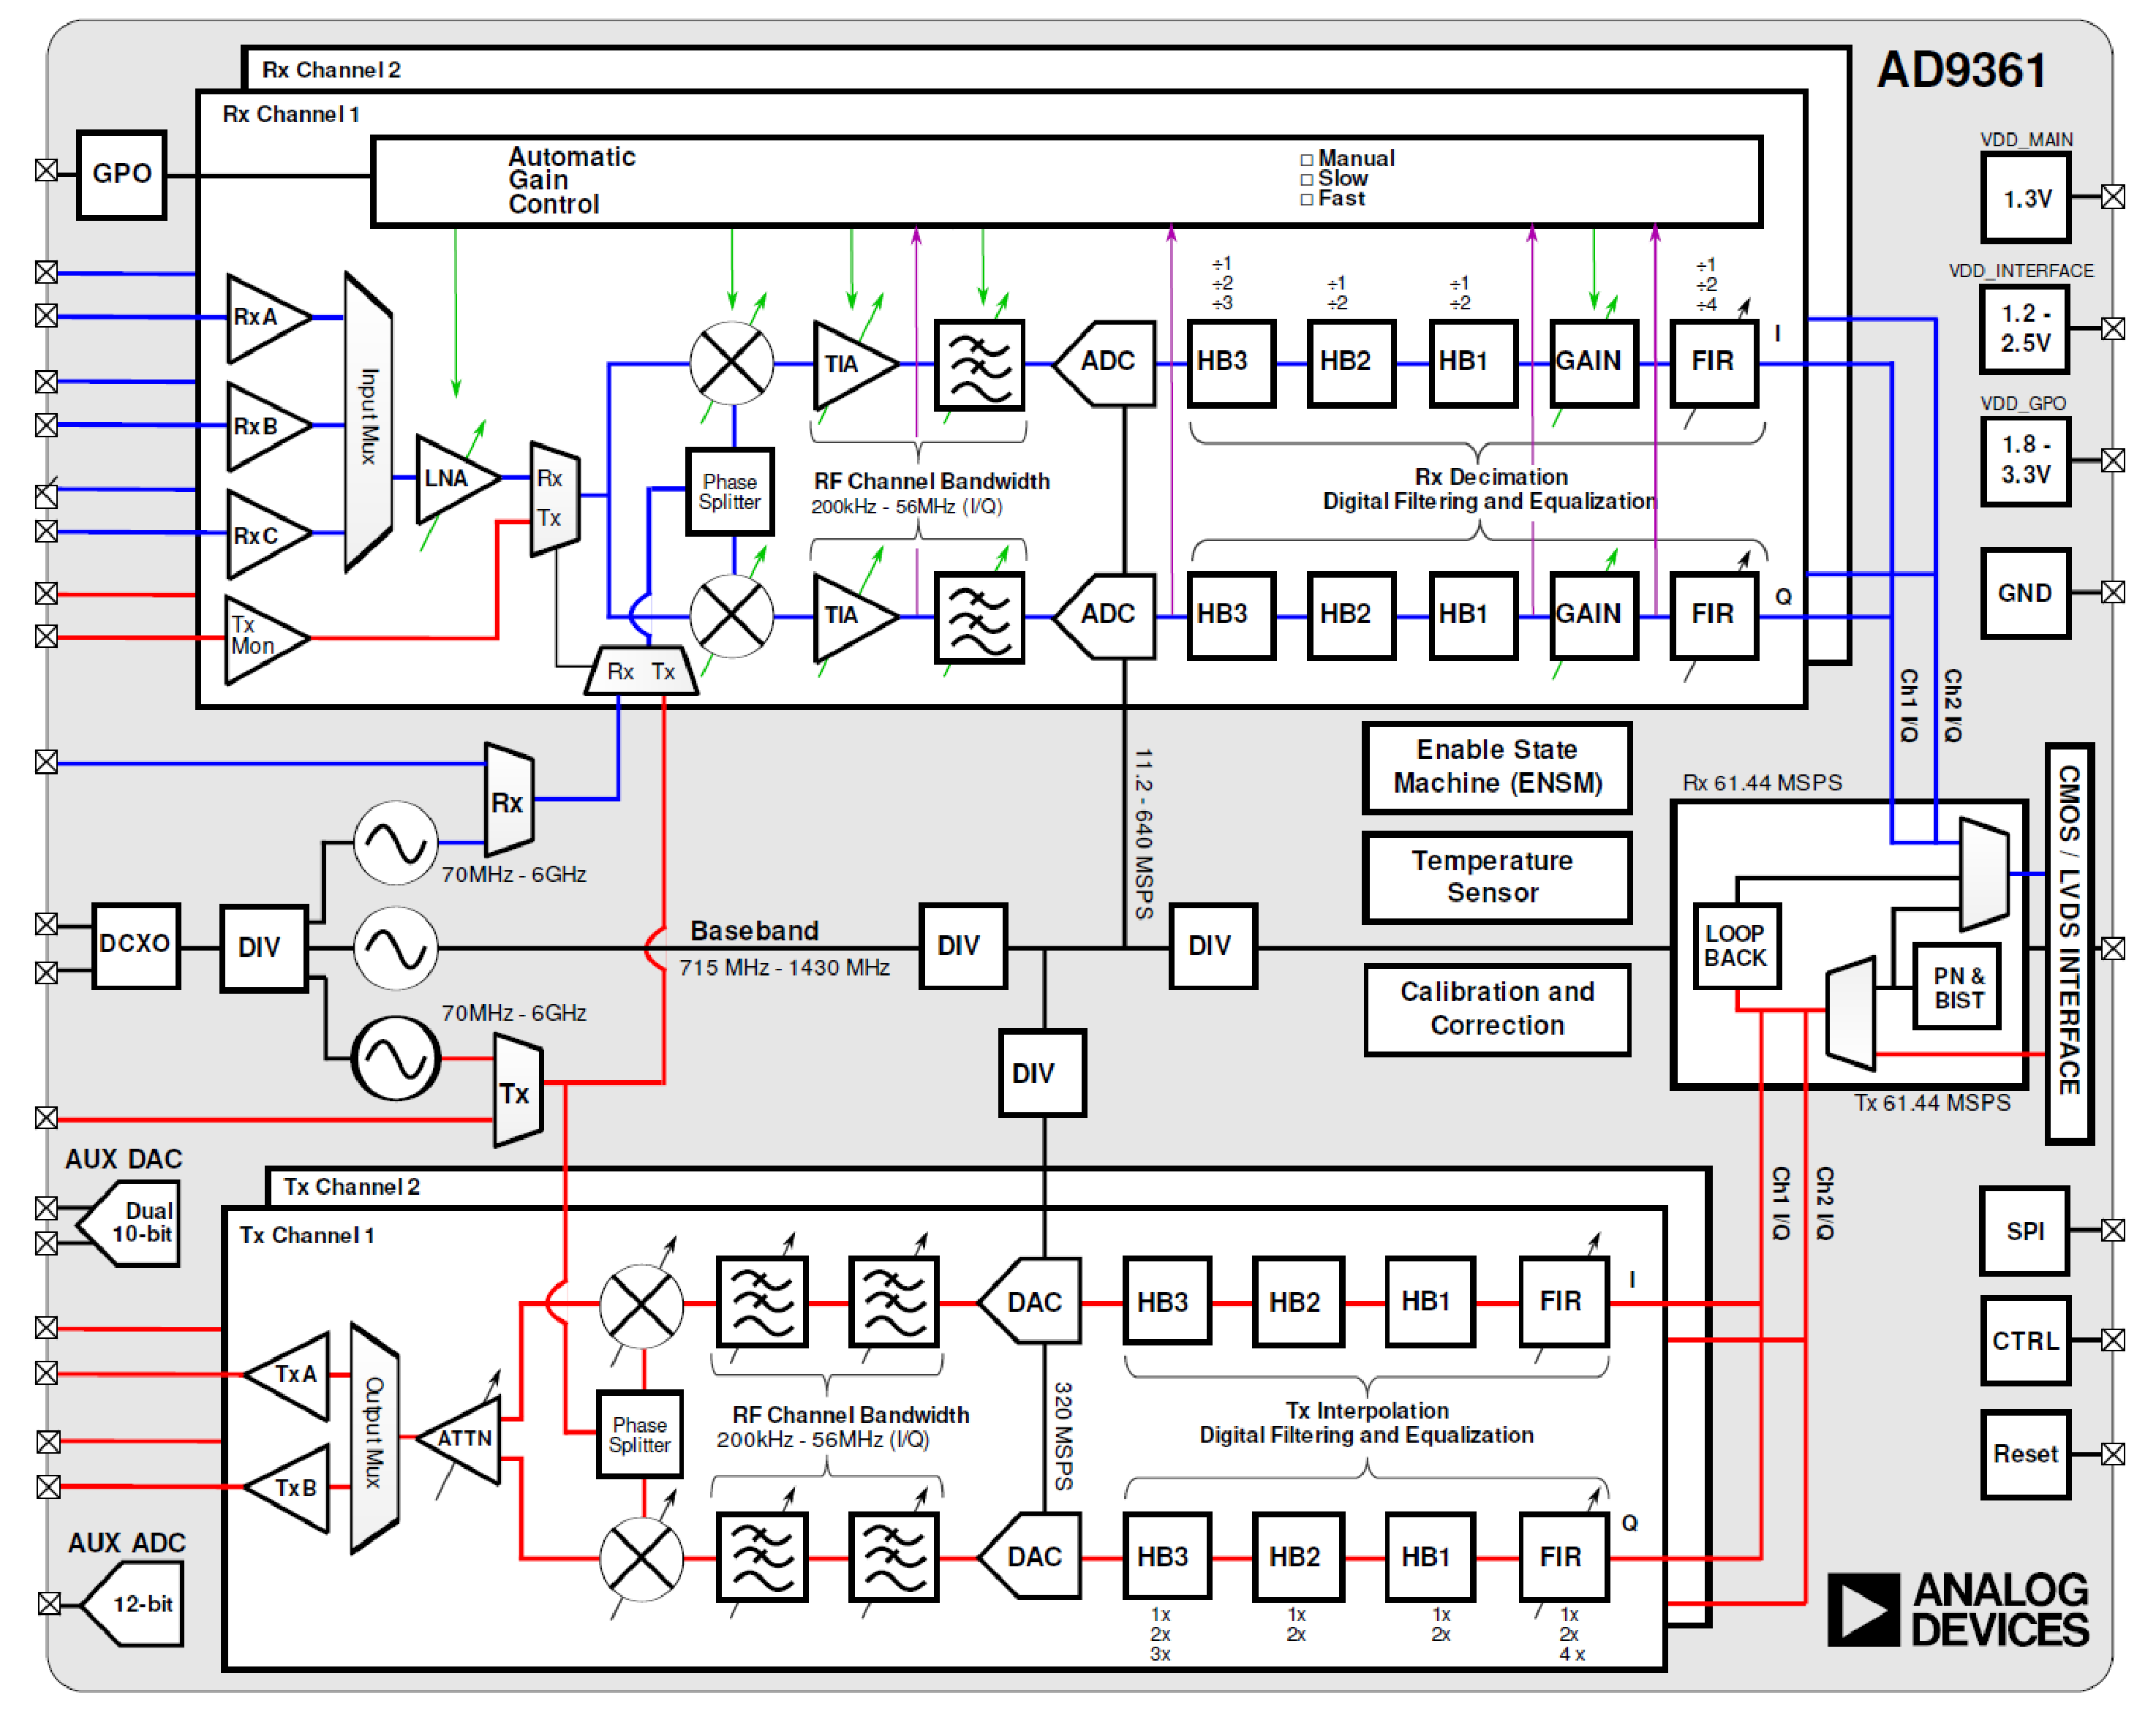
\includegraphics[width=0.65\textwidth]{./figures/ad9361_block_diagram}
    \caption{ AD9361 Block Diagram
    \label{fig:ad9361blk}}
\end{figure}

\subsubsection{Filtering}

In both receiver and transmitter there are:
\begin{description}
	\item[Receiver] \hfill \\
	\begin{itemize}
		\item Low pass filter : band shape to reduce adjacent-channel interference.
		\item Decimation Filter: up convert from the digital baseband rate (64.11MSPS max) to the actual ADC (640MSPS) rate.
	\end{itemize}
	\item[Transmitter] \hfill \\
\begin{itemize}
		\item Low pass filter : remove sampling artifacts
		\item Interpolation Filter : down convert from the digital baseband rate (64.11MSPS max) to the actual DAC (320MSPS) rate.
	\end{itemize}
\end{description}

In both digital and analog implementations these filters have impact the magnitude and the phase in passband, such behavior must be compensated in the system, and this compensation is usually done inside the 128-tap FIR filter. The FIR filter is not only used for low pass filter realization but also to compensate for magnitude and phase impacts created by the analog and digital half band filters in the desired baseband area.

These filters depend in various other systems to work properly, such systems are sample rates, clock, data rates which sets the half band filters, and the desired RF bandwidth, which sets the analog filters. the process of loading a filter and after changing anything in the system will negatively affect the overall baseband performance.

There is a filter too created by analog devices,which designs a low-pass filter and sets the FIR coefficients in order to ensure compensation for magnitude and phase changes in the analog or half band filters.

\subsubsection{Clocking}

%reescrever
The AD9361 has a series of internal PLL to generate and manipulate clock signals. There are fractional-n PLLs that generate the transmitter and receiver LO frequencies and there are the baseband PLL (BBPLL) used for the data converters, digital filters and I/O ports. All the frequency signals are generated using these PLLs clock outputs.

All the PLLs require a reference clock input and for this there is the digitally controlled oscillator (DXCO) function, which is an in-chip programmable and variable capacitor, such capacitor can tune the crystal frequency variance before entering the system, having a precision of +/- 6 ppm it results in a more accurate reference clock and can be used, if needed, for synchronization purposes. this function can also be used together with the on-chip temperature sensor to provide temperature compensation depending enviroment in which the chip will be used. For the reference clock there are two options:

\begin{description}
	\item[External Oscillator] \hfill \\
	In this option and external clock signal can be connected in the XTALP pin (Leaving the XTALP pin unconnected), this external clock frequency may vary from 10 MHz to 80 MHz. Such type of setup is needed when a wireless basestation (BTS) reference clock is locked to a master clock, and in such systems there is no or less need for clock synchronization.

	\item[Dedicated Crystal] \hfill \\
	In this option a dedicated crystal, with frequency varying from 19 MHz to 50 MHz, is connected in the XTALP and XTALN pins. This setup is usually used in wireless user equipment (UE), which do not need to be locked to a master clock but they do need to adjust periodically the LO frequency in order to maintain a connection with a BTS. The BTS periodically informs the UE of its frequency error relative to the BTS and the BBP can make adjustments to the reference clock and thus adjust the LO frequency if needed.

\end{description}

\begin{figure}[htbp]
    \centering
    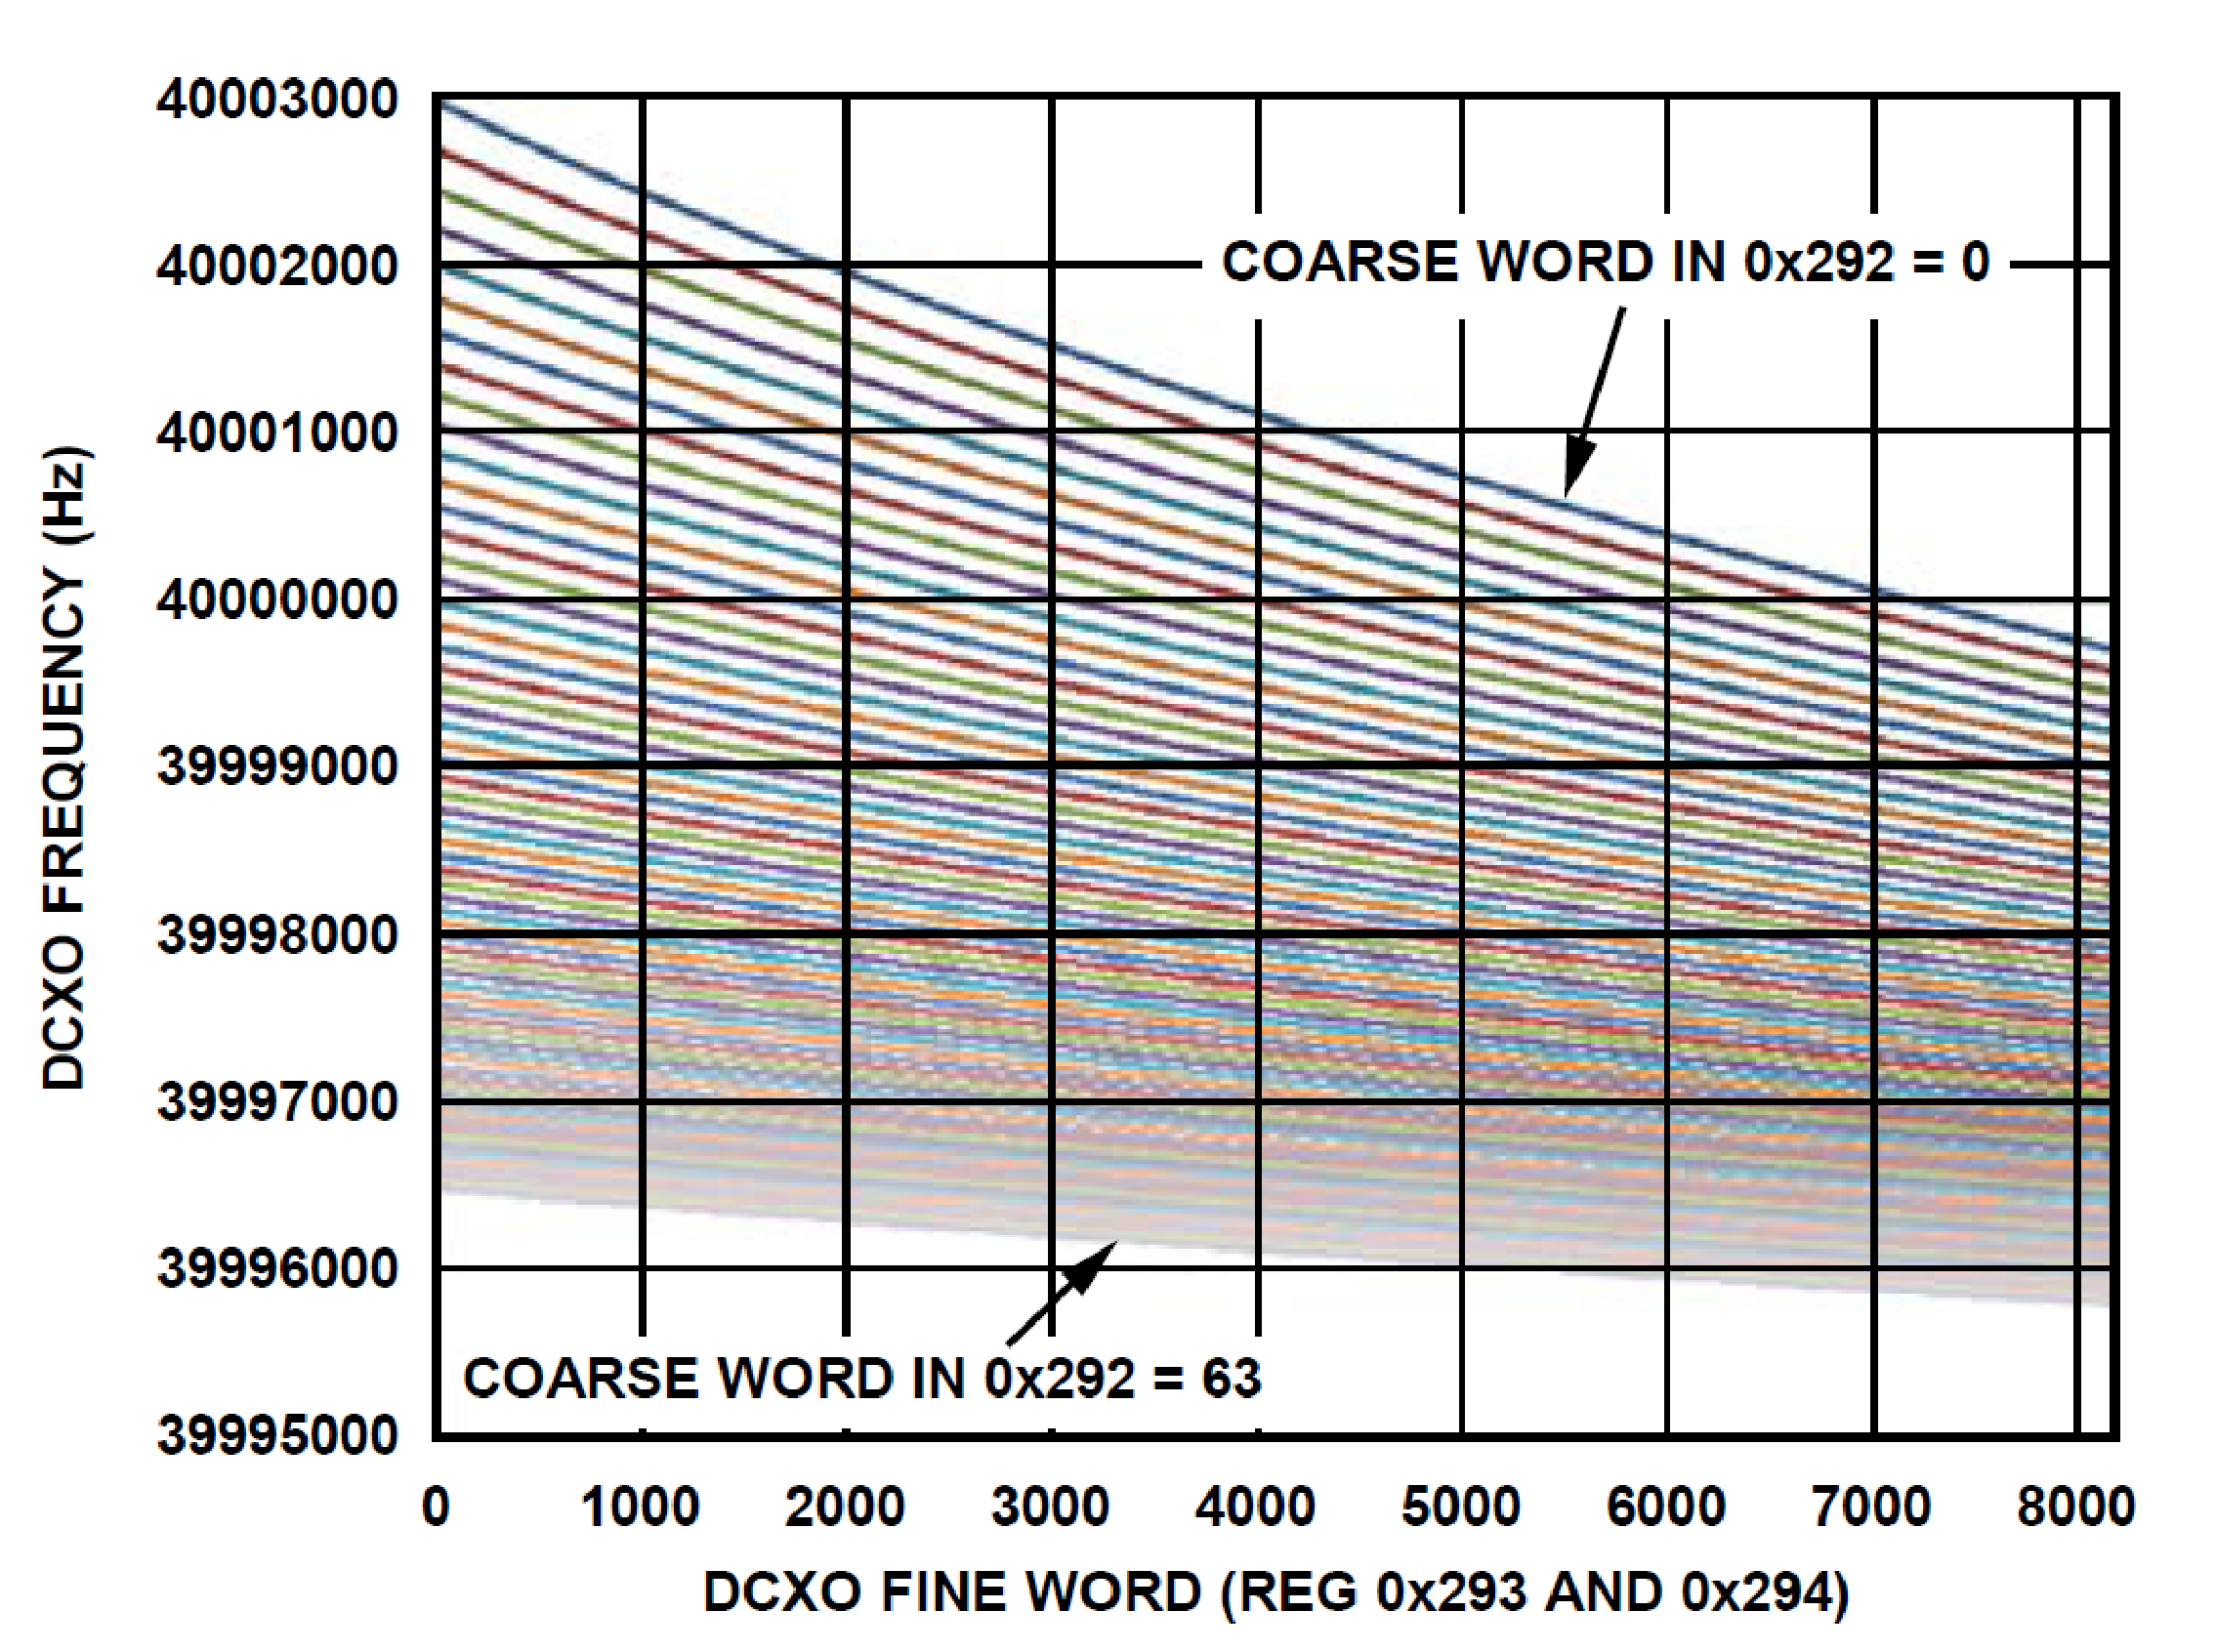
\includegraphics[width=0.65\textwidth]{./figures/dcxo_graph}
    \caption{ DCXO Behavior Graph
    \label{fig:pll}}
\end{figure}

\subsubsection{Synthesizers}

\begin{description}
	\item[RF PLLs] \hfill \\
	The AD9361 contains two identical synthesizers to generate the required LO signals for the RF signal path, one for the receiver and one for the transmitter. The PLL synthesizers are fractional-n PLLs with completely integrated VCOs and loop filters, requiring no other external components. In TDD operation mode, the synthesizers turn ON and OFF appropriate for the TX and RX frames, however in FDD TX PLL and RX PLL are activated at the same time.

	\item[BB PLL] \hfill \\
	The AD9361 contains also a baseband PLL synthesizer, which generate all the baseband related clock signals. The BBPLL feeds all the baseband related clock signals to ADC, DAC (Sampling Clock), DATA\_CLK signal and all data framing signals. This PLL has a frequency range from 700 Mhz to 1400 Mhz, and can be changed based on system requirements.

\end{description}

\begin{figure}[htbp]
    \centering
    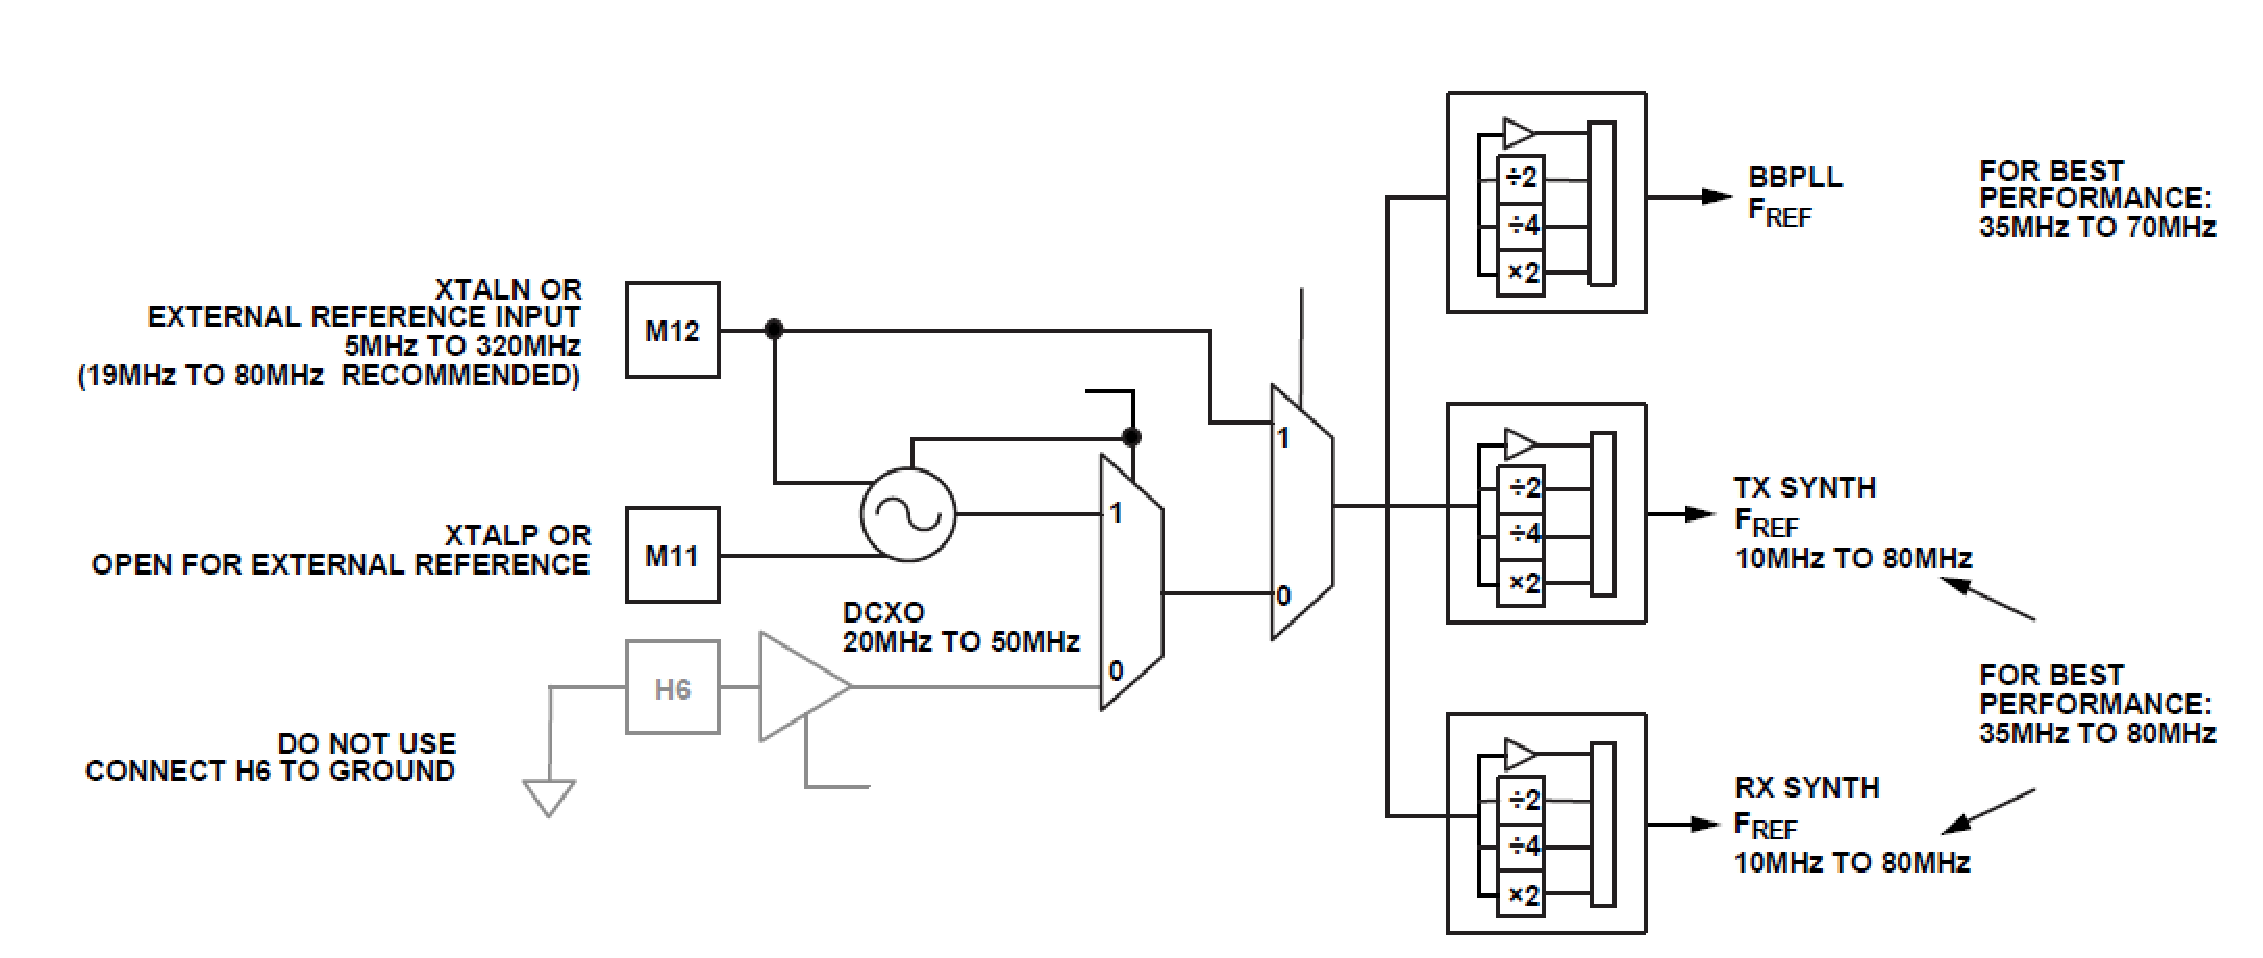
\includegraphics[width=0.65\textwidth]{./figures/pll_ref_block}
    \caption{ AD9361 PLL Reference Block Diagram
    \label{fig:pll}}
\end{figure}

\subsubsection{Digital Data Interface}

The AD9361 uses parallel data ports to transfer data between the device and the BBP. These data ports can be configured either single-ended CMOS format or LVDS format (used in this work). Both formats can be configured in multiple arrangements to adequate the system requirements for data transfer and connections. These arrangements can be of single port data bus, dual port data bus, single data rate, double data rate and other various combinations compatible with the device.\\
Bus transfers are controlled using hardware handshake signalling, these two ports can be operated in TDD (bidirectional) or FDD (full duplex) where half of the bits are used for transmitting and the other half is used for receiving. The interface can also be configured to use only one of the data ports ( usually used in applications that do not require high data rates or samples).\\
The communication between the BBP processor and the AD9361 rely on some signals to properly work, which are DATA\_CLK, FB\_CLK and RX\_FRAME, its operation is detailed below:

\begin{description}
	\item[DATA\_CLK Signal] \hfill \\
	RX sends the signal DATA\_CLK to the BBP, which can be used when receiving data. DATA\_CLK can be used to control data sampling time, which can be single data rate (data is captured on rising clock edge) or double data rate (data is captured on both rising and falling clock edges). This can be applied using single or dual data port.

	\item[FB\_CLK Signal] \hfill \\
	The FB\_CLK signal must have the same frequency and duty cycle as DATA\_CLK and like DATA\_CLK it is used as timing reference for the interface. FB\_CLK allows source synchronous with rising edge capture for burst control signals and can be used like DATA\_CLK for rising edge, single data rate mode or in both edge capture, double data rate mode for transmit signal bursts.

	\item[RF\_FRAME Signal] \hfill \\
	The RF\_FRAME signal is generated by the device whenever the receiver outputs valid data. RF\_FRAME has two modes:
	\begin{itemize}
		\item \textbf{Level Mode:} RF\_FRAME stays high as long as the data is valid.
		\item \textbf{Pulse Mode:} RF\_FRAME pulses with 30% duty cycle.
	\end{itemize}
	The BBP must provide a TX\_FRAME that indicates beginning of a valid data transmission with a rising edge. The TX\_FRAME operates similarly as the RF\_FRAME, on Level Mode or Pulse Mode.

\end{description}

\begin{figure}[htbp]
    \centering
    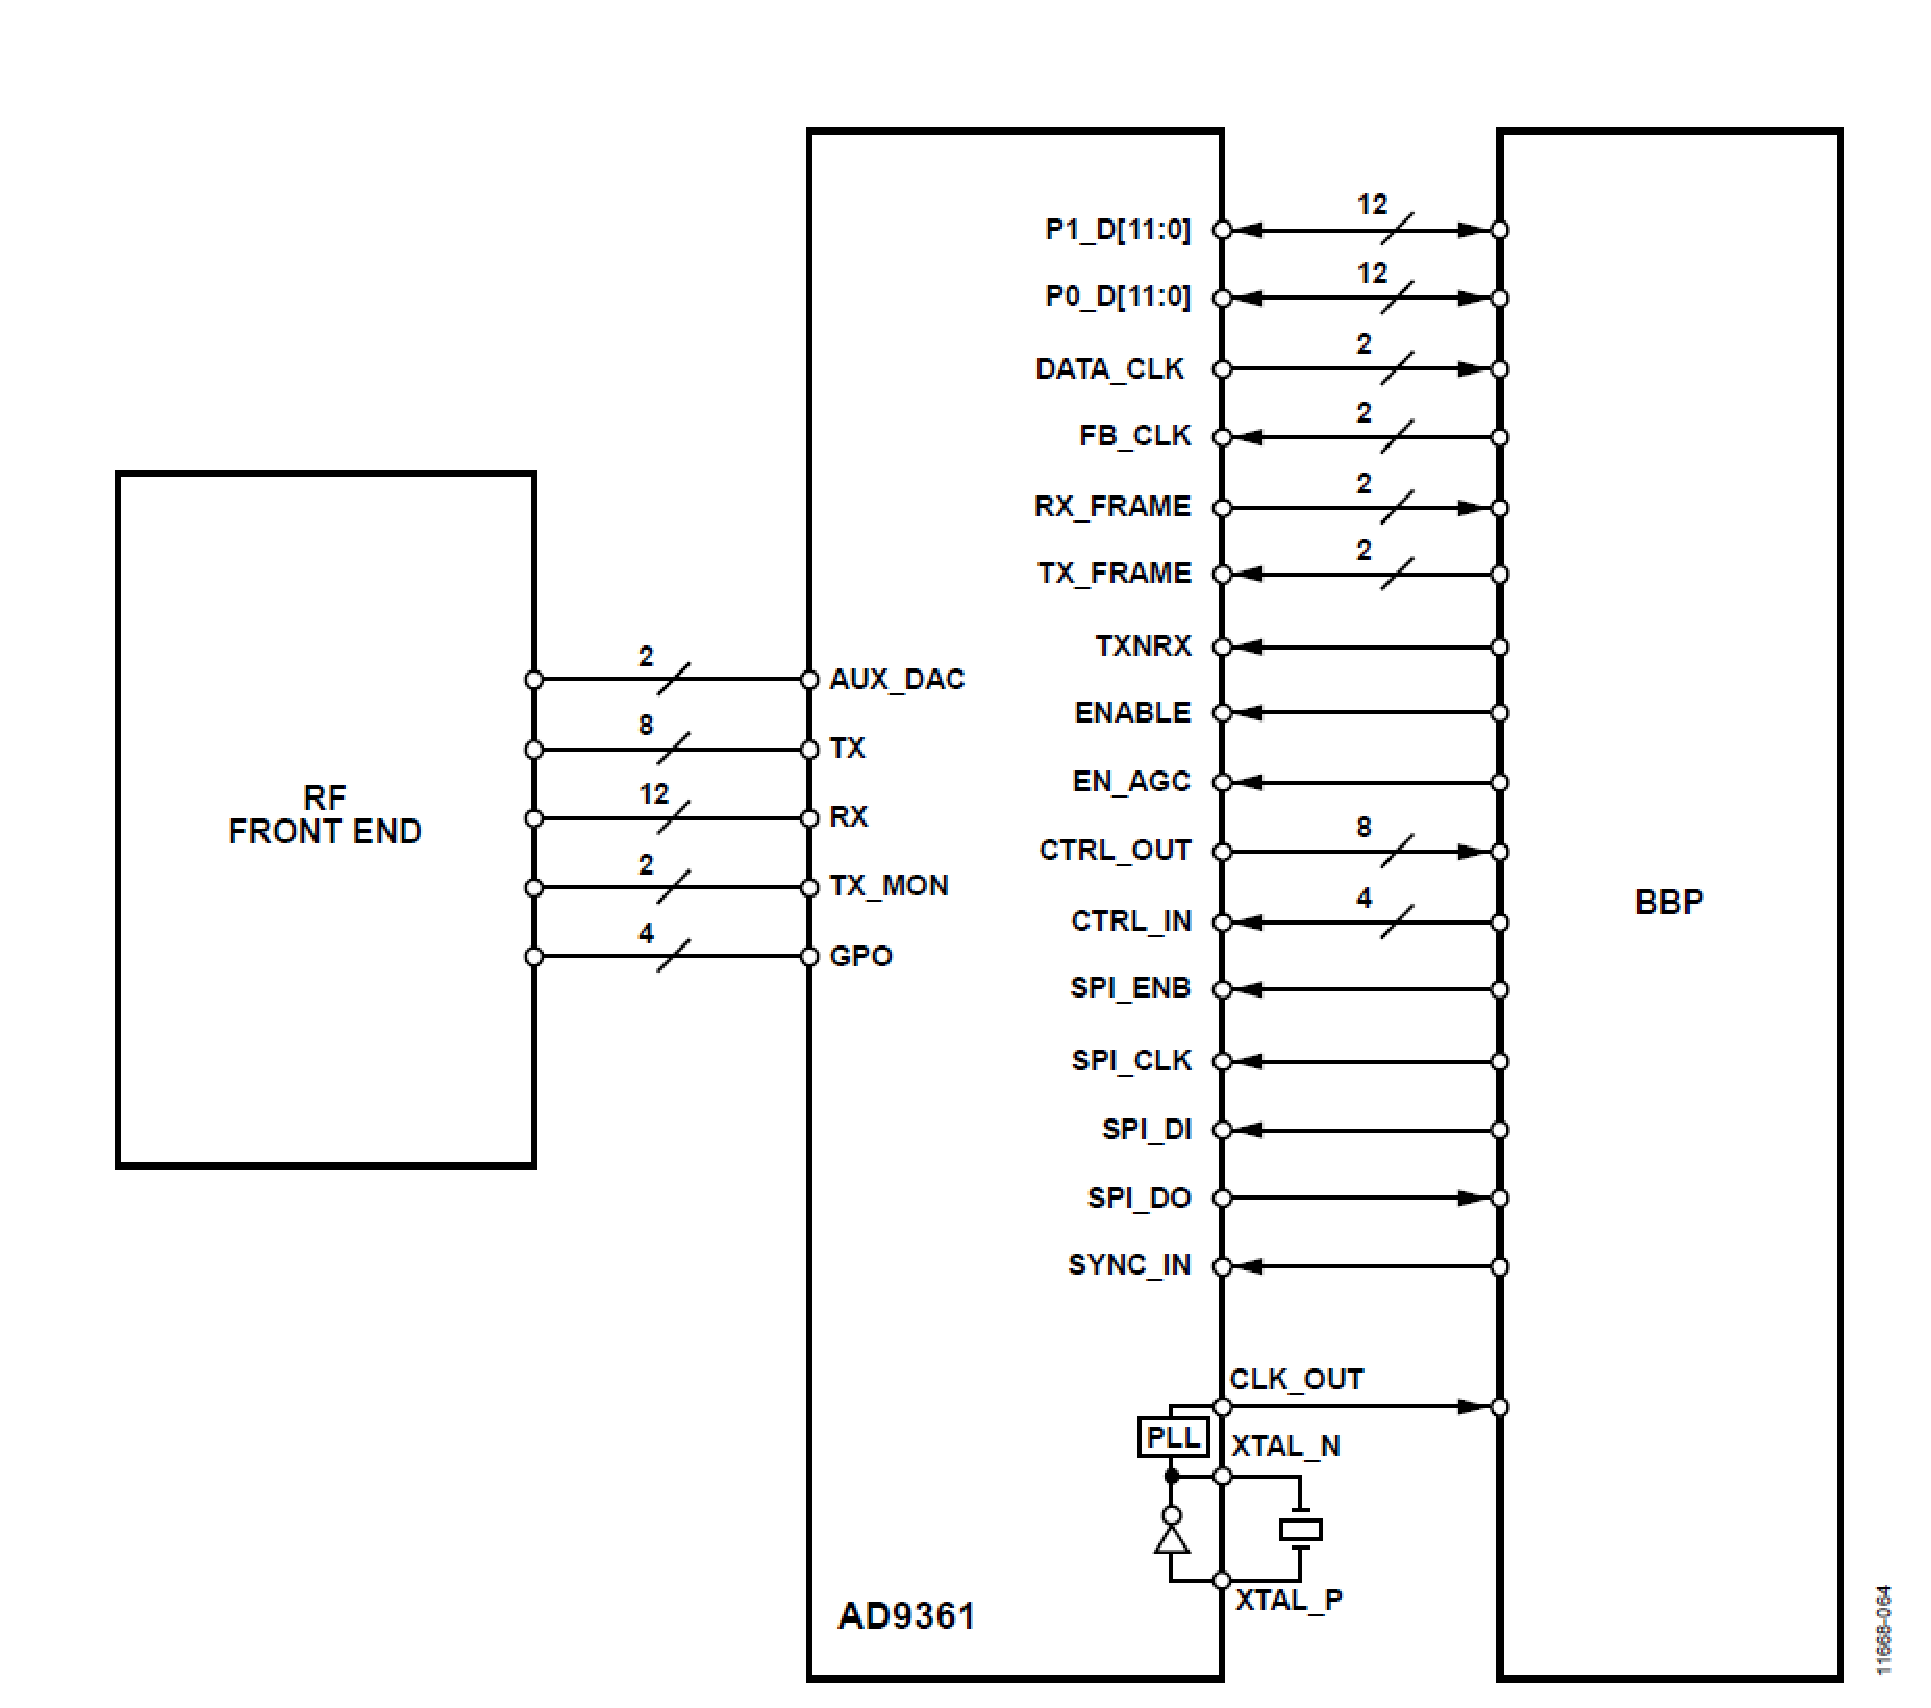
\includegraphics[width=0.65\textwidth]{./figures/ad9361_digital_interface}
    \caption{ AD9361 Digital Data Interface
    \label{fig:ad9361diginterface}}
\end{figure}


\subsubsection{Enable State Machine}

The AD9361 has an Enable State Machine (ENSM) which allows real-time control over the current state of the device. The device can be place in several states like:

\begin{itemize}
		\item \textbf{Wait:} Power save, synthesizers disabled.
		\item \textbf{Sleep:} Wait with all clocks and BBPLLs disabled.
		\item \textbf{TX:} TX chain enabled.
		\item \textbf{RX:} RX chain enabled.
		\item \textbf{FDD:}TX and RX chains enabled.
		\item \textbf{Alert:} Synthesizers enabled.
	\end{itemize}
	This ENSM can be controlled either by SPI or PIN (GPIO for example), where the SPI control mode is for a non real-time operation and the PIN control mode is for a much faster and real-time control.


\begin{description}
	\item[SPI Control Mode] \hfill \\
	In SPI control mode, the BBP writes registers asynchronously by using SPI protocol to access the addresses, and by writing these registers the state machine advances the current state to the next state. SPI communication is considerece asynchronous to the DATA\_CLK because the SPI\_CLK can be derived from another clock source, where BBP and the device does not share the same clock source. This control method is recommended when there is no need for a real-time control.

	\item[Pin Control Mode] \hfill \\
	In Pin control mode, there are pins dedicated to activate some states of the ENSM, like ENABLE pin and TXNRX pin, this mode allows a real-time control of the current state. This method is recommended in a system where the BBIC has extra pins to spare with the real-time control outputs, this 2-wire interface can control the state of the device.
	To advance the current state to the next state of the ENSM, the enable function of the ENABLE pin can be driven by either pulse or level,if the pulse is used the minimum width of the pulse needs to be equal as the FB\_CLK cycle.
	In FDD mode, the ENABLE and TXNRX pins can be remapped to be used as real-time control of the TX and RX data transfers. In this mode ENABLE enables or disables the receive signal and TXNRX enables or disables the transmit signal, using such mode  causes the ENSM to be removed from the system for data flow control and is replaced by these pins.

\end{description}

\begin{figure}[htbp]
    \centering
    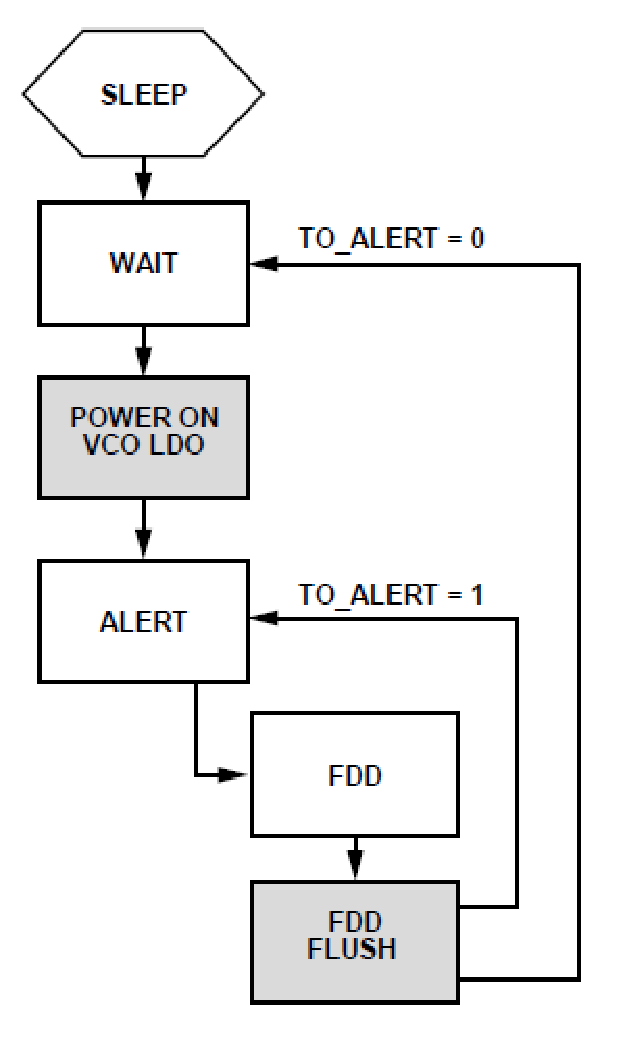
\includegraphics[width=0.65\textwidth]{./figures/fdd_ensm}
    \caption{ FDD Enable State Machine
    \label{fig:pll}}
\end{figure}

\begin{figure}[htbp]
    \centering
    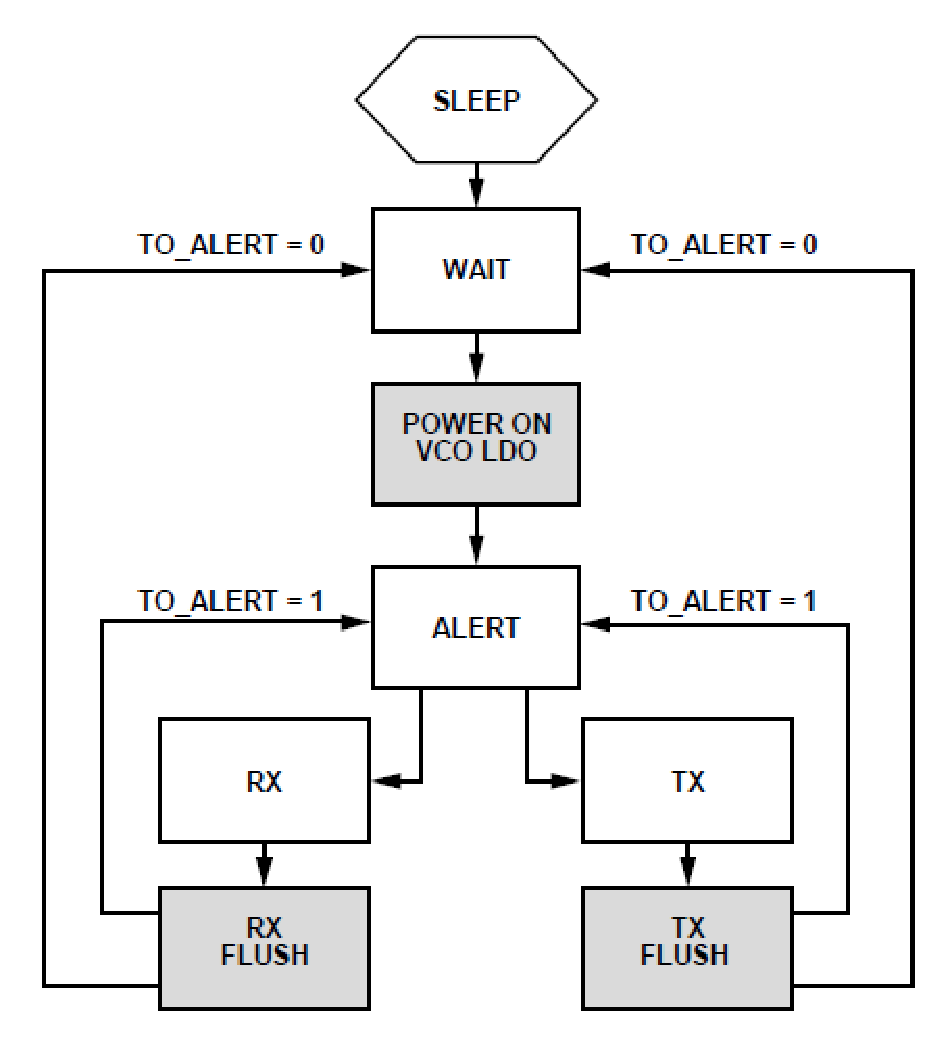
\includegraphics[width=0.65\textwidth]{./figures/tdd_ensm}
    \caption{ TDD Enable State Machine
    \label{fig:pll}}
\end{figure}


\subsubsection{SPI Interface}

The AD9361 uses a SPI interface for communication with the BBP. Throught SPI is possible to access all the device registers. The PSI interface can be configured as a 4-wire interface with dedicated transmit and receive pins, duplex, or as 3-wire interface with bidirectional data port.
Write commands have a 24-bit format where the first six bits are for setting the bus direction and number of bytes to transfer, the next 10 bits set the address where the data is to be written and the final eight bits are the data to be transferred to the specific register address (MSB to LSB), a LSB-first format is also supported.
Read commands follow a similar format, the difference is that the first 16 bits are transferred on the SPI\_DI pin and the final eight are read from the AD9361, either using SPI\_DO (4-wire interface) or SPI\_DI (3-wire interface).

\subsubsection{Auxiliary Converters}

\begin{description}

	\item[AUXADC] \hfill \\
	The AD(361 contains an auxiliary ADC that can be used to monitor some system functions such as temperature or power output, it is a 12-bit converter and has an input range of 0V to 1.25V. The SPI can read the last value latched at the output of the ADC when it is enabled for use, there is also a multiplexer that permits to select between AUXADC and built-in temperature sensor.

	\item[AUXDAC1 and AUXDAC2] \hfill \\
	The AD(361 also has two identical auxiliary DACs which can be used to provide power amplifier (PA) bias or other system functionality. Both the DACs are 10-bit wide and have an output range of 0.5 V to 0.3V and have a current drive of 10mA. The DACs can be directly controlled by the ENSM.

\end{description}

\subsubsection{Applications}


\subsection{FMCommS2}

FMCommS2 is basically evaluation board for the AD9361 that has a FPGA Mezzanine Card (FMC) connector for interfacing with the BBP (Usually FPGA). The FMComms2 has 5 SMA connectors, 2 for Rx, 2 for Tx and one for external reference clock input. The FMComms2 provides a 2x2 RF configuration, extended from the AD9361, and has  a narrow tuning range balun, which is performance optimized for 2.4GHz.
The FMComms2 is a transceiver intended for use in RF applications such 3G or 4G BTS or SDR. Its programmability and wideband capability make it ideal for broad range of transceiver applications and make it very attractive for the new C-RAN paradigm.

\begin{figure}[htbp]
    \centering
    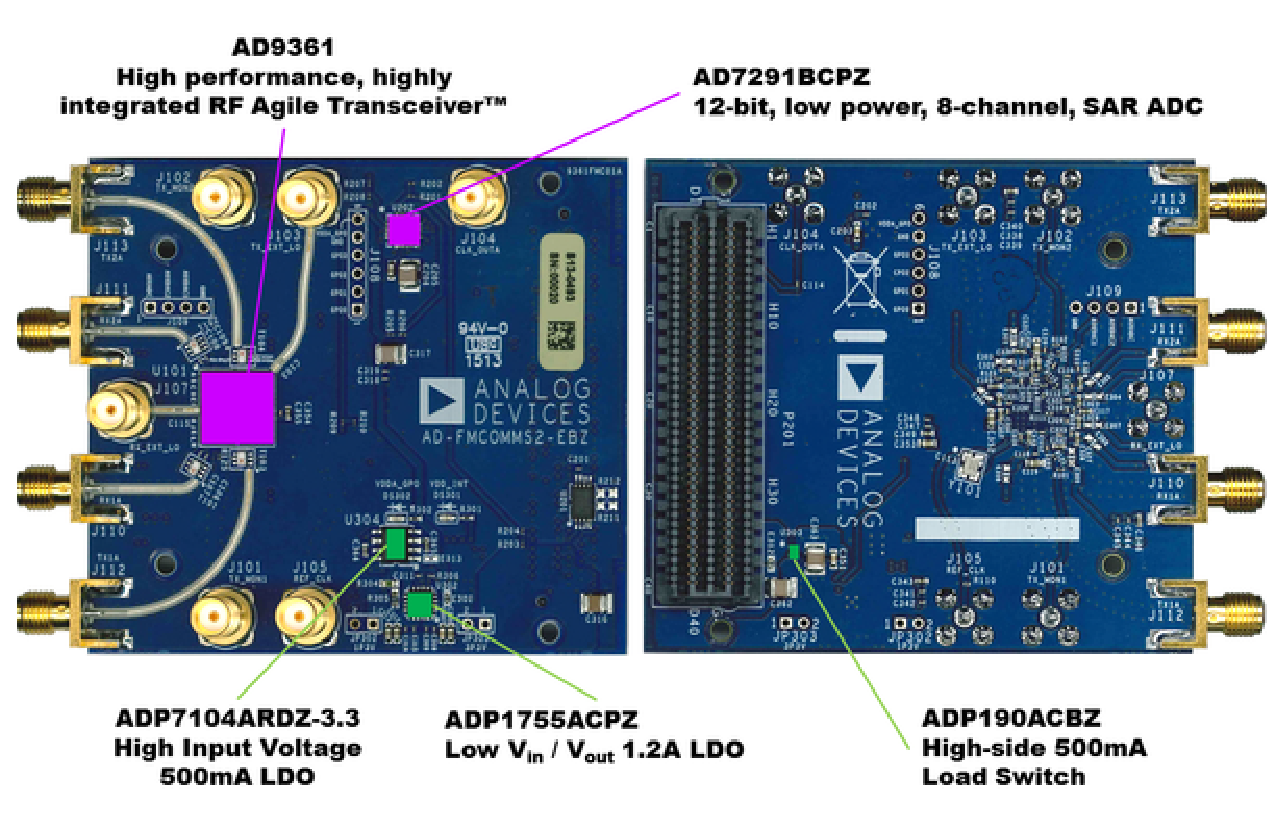
\includegraphics[width=0.65\textwidth]{./figures/fmcomms2_pic}
    \caption{ FMComms2 and its components
    \label{fig:fmcomm}}
\end{figure}


\subsubsection{Functional Overview}

The Block diagram show that there are 4 main functional partitions - receiver path, transmit path, clocking and power supply. Since the FMComms2 incorporates and extends the basic functionalities of the AD9361, thus the data path is fully integrated into the AD9361.

\begin{figure}[htbp]
    \centering
    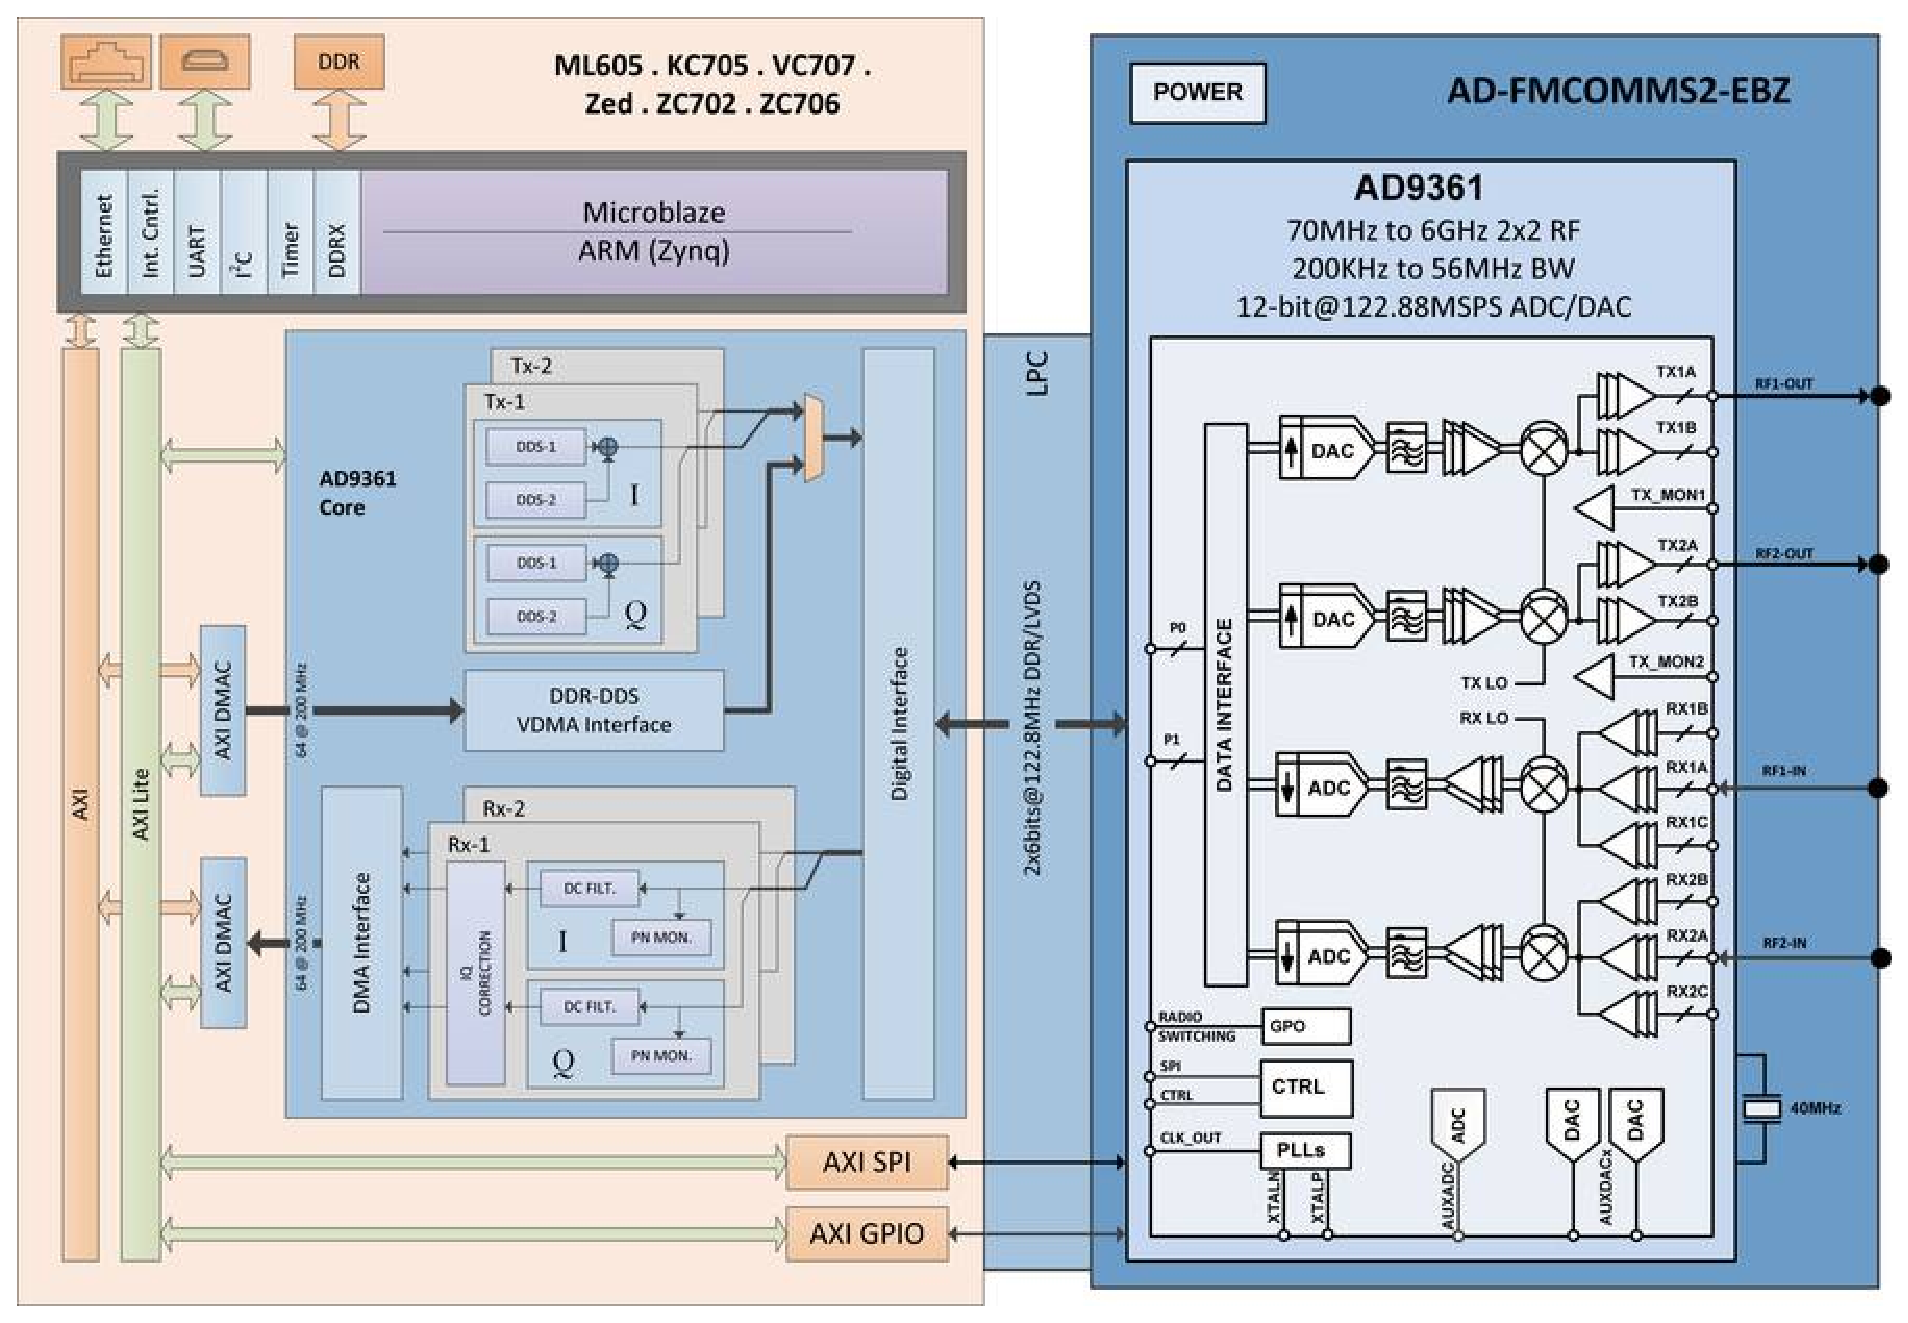
\includegraphics[width=0.65\textwidth]{./figures/fmcomms2_bd}
    \caption{ FMComms2 and FPGA Block Diagram
    \label{fig:fmcommbd}}
\end{figure}



\begin{description}
	\item[Receive] \hfill \\
	\begin{itemize}
		\item Support up to 2 direct conversion RF receiver channels.
		\item Fully integrated frequency synthesizers (including loop filter).
		\item Data path consists in LNA, Demodulator, LPF, ADC and digital filters.
		\item \textit{AGC:} quadrature calibration and DC offset calibration.
		\item \textit{NF:} 2.5 dB at 1Ghz.
		\item \textit{ADC:} Continuous time sigma-delta ( $\Sigma - \Delta$), 640 MSPS.
		\item \textit{Digital FIlter:} 128 COmplex taps with decimation between 2 and 48.
		\item \textit{Gain:} 1dB step size, 80 dB analog Range, 30 db digital range (post ADC scaling).
		\item On-chip sensor for temperature corrected RSSI.
	\end{itemize}

	\item[Transmit] \hfill \\
\begin{itemize}
		\item Supports up to 2 direct conversion RF transmit channels.
		\item Fully integrated frequency synthesizers (including loop filter).
\item Data path consists of digital filters, DAC and modulators.
		\item \textit{Digital FIlter:} 128 complex taps with interpolation between 2 and 48.
		\item \textit{Gain:} 0.5 dB step size, 86 dB range.
		\item \textit{ADC:} 340 MSPS.
	\end{itemize}

	\item[Clocking] \hfill \\
		The FMComms2 board has a integrated crystal oscillator of 40 Mhz and has a SMA input for external clock input.

	\item[Control/Monitor] \hfill \\
		The board allows real time control and monitoring via dedicated pins, such pins functionality are programmable. The control and monitor programming configuration is specified in the ad9361 section \cite{sec:ad9361}.

\end{description}

\subsection{Basic Mathematical Background}

\subsubsection{Complex Modulation}

\begin{eqnarray}
	I = sin(\omega \times t)\\
	Q = cos(\omega \times t)
\end{eqnarray}

\begin{equation}
	cos(\omega \times t) = sin(\frac{\pi}{2} - (\omega \times t))
\end{equation}

then:

\begin{eqnarray}
	I = sin(\omega \times t)\\
	Q = sin(\frac{\pi}{2} - (\omega \times t))
\end{eqnarray}

These are the two signals coming out of the DAC, two sine waves, phase offset from each other, wich is called IQ.

\subsubsection{Basic Modulation Mathematics}

Start to modulating signal from a amplitude perspective:

\begin{eqnarray}
LO_I = A_x cos(k)\\
LO_Q = B_x sin(k)
\end{eqnarray}

We still have the carrier:

\begin{equation}
LO_I = cos(\omega) ; LO_Q = sin(\omega)
\end{equation}

Will result:

\begin{eqnarray}
LO_I \times I = A_x cos(k) \times sin(\omega)\\
LO_Q \times I = B_x sin(k) \times cos(\omega)
\end{eqnarray}


That gives the output:

\begin{equation}
x(t)=A_x cos(k)\times sin(\omega)+ B_x sin(k)\times cos(\omega)
\end{equation}

This does not match with any trigonometrical identities and it is easier to use Euler\'s formula:

\begin{eqnarray}
sin(x)=(\frac{1}{2}e^{-jx} - \frac{1}{2}e^{jx})\\
cos(x)=(\frac{1}{2}e^{-jx} + \frac{1}{2}e^{jx})
\end{eqnarray}

Therefore:

\begin{equation}
x(t)=A_x (\frac{1}{2}e^{-jk} + \frac{1}{2}e^{jk})\times (\frac{1}{2}e^{-j\omega} - \frac{1}{2}e^{j\omega})+ B_x (\frac{1}{2}e^{-jk} - \frac{1}{2}e^{jk})\times (\frac{1}{2}e^{-j\omega} + \frac{1}{2}e^{j\omega})
\end{equation}

\begin{equation}
x(t)=\frac{A}{2} (e^{-jk} + e^{jk})\times (e^{-j\omega} - e^{j\omega})+ \frac{B}{2} (e^{-jk} - e^{jk})\times (e^{-j\omega} + e^{j\omega})
\end{equation}

If we expand we get:

\begin{equation}
x(t)=\frac{1}{2} ((Ae^{-jk-j\omega} + Ae^{jk-j\omega} - Ae^{-jk+j\omega} - Ae^{jk+j\omega}) + (Be^{-jk-j\omega} - Be^{jk-j\omega} - Be^{-jk+j\omega} + Be^{jk+j\omega}))
\end{equation}


And then:

\begin{equation}
x(t)=\frac{1}{2} ((A+B)e^{-jk-j\omega} + (A-B)e^{jk-j\omega} - (A-B)e^{-jk+j\omega} - (A+B)e^{jk+j\omega})
\end{equation}

It is possible to rearrange as:

\begin{equation}
x(t)=\frac{1}{2} \times ((A+B)(e^{-jk-j\omega} - e^{jk+j\omega}) + (A-B)(e^{jk-j\omega} - e^{-jk+j\omega}))
\end{equation}

And then:

\begin{equation}
x(t)=(\frac{A+B}{2} )(sin(k+\omega)) + (\frac{A-B}{2} )(sin(k-\omega))
\end{equation}

If this due to amplitude mismatch, this creates an image on the other side of the local oscillator.

\section{Setup}

\subsection{Overview}

As stated before, C-RAN is still in development and it is not already a solid
standard, so exploring setups and their feasibility is very interesting to
increase the ways to implement this new standard in countries which does not
have a very good infrastructure.

The first setup thought was using the ML605 FMC LPC connector and the FMComms2,
this setup was very important because in it I could understand how to integrate
the board design with the need of the project. Then the device was moved to the
FMC HPC connector and the design with the ML605 was finished.\\

After getting the experience with ML605 and ISE design tools, it was time to use
a more updated board and design tool, thus the idea of porting the initial design from
ML605 to the VC707 board came. Since ISE has no support for VC707 and is a
software with its development halted, going to the most updated tool from Xilinx
is natural, so the second setup is using vivado design tools and VC707 with FMC
HPC connector and FMComms2.\\

Another thing to give attention is that with ISE the design flow was more manual and if there was the need to rebuild a project almost from the scratch, just with the HDL source files, the other necessary ips should be created and configured again, which took a lot of time, but with Vivado the block diagram design flow and the .tcl scripts became more popular, they existed in ISE however they were not popular. With the TCL scripts it is possible to create project, import files, instantiate and configure both user and default IPs, as well as run synthesis, implementation and generate bitstream steps, which saves a lot of time in development.\\

%figura das duas fases do SETUP downlink e Uplink
\begin{figure}[htbp]
    \centering
    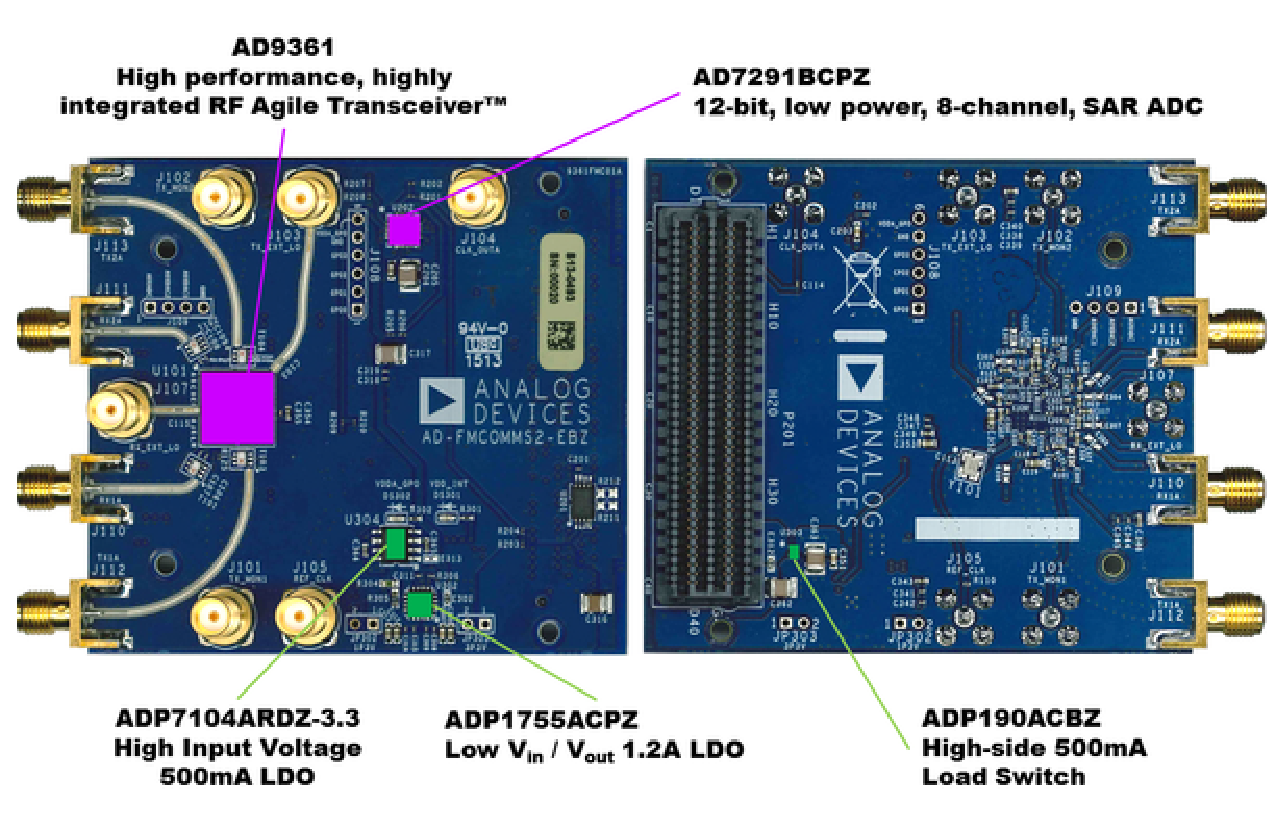
\includegraphics[width=0.65\textwidth]{./figures/fmcomms2_pic}
    \caption{ FMComms2 and its components
    \label{fig:fmcomm}}
\end{figure}

\begin{figure}[htbp]
    \centering
    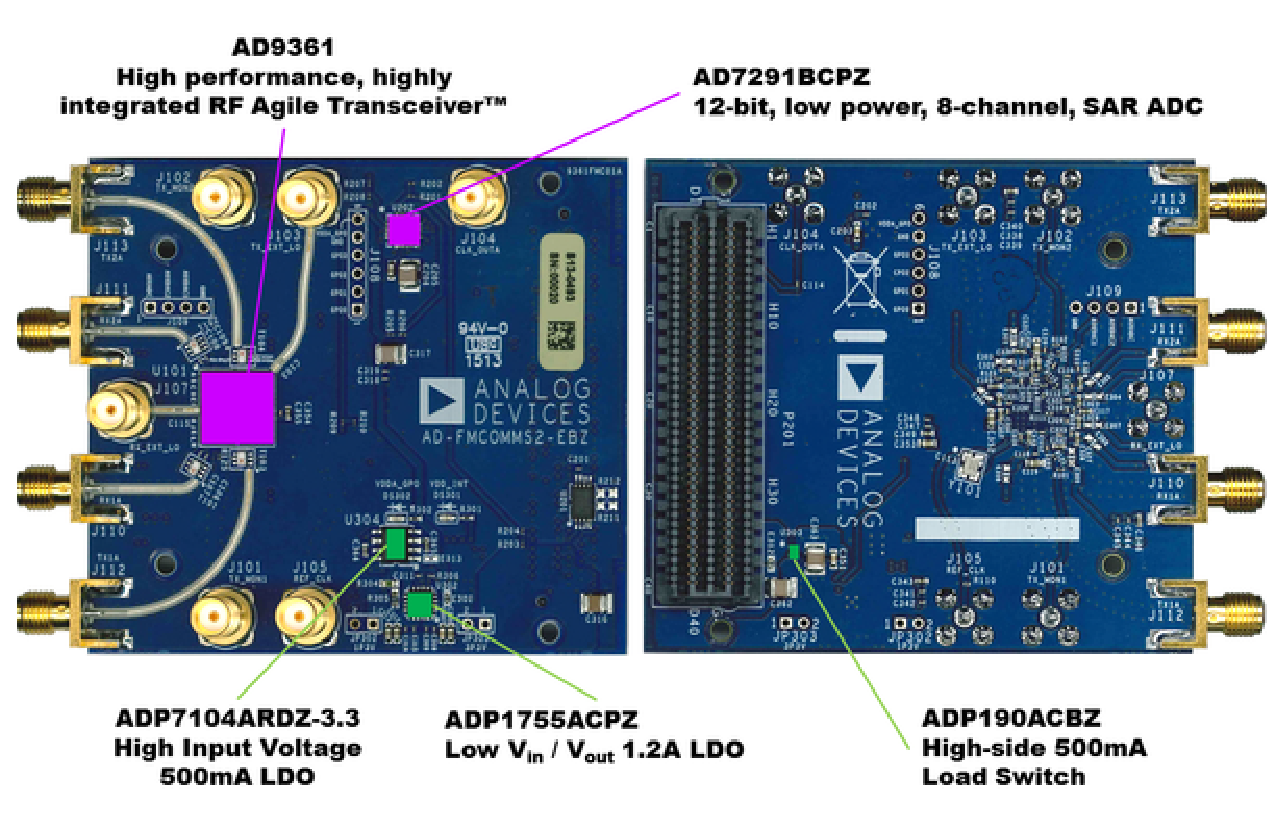
\includegraphics[width=0.65\textwidth]{./figures/fmcomms2_pic}
    \caption{ FMComms2 and its components
    \label{fig:fmcomm}}
\end{figure}

\subsection{Integration between FPGA and FMComms2}

The first problem encountered in the development was the integration, since the
company make a example project available and the IP cores for download it appear
to be an easy job, however, for study purposes and for a simpler design it is
better to begin a bottom up approach and so it was did.

This approach was used in both ML605 and VC707 and it consists in basic steps:

\begin{enumerate}
    \item Analyse which ports have to be connected
    \item Analyse which Communications protocols are needed to communicate with the device;
    \item Analyse the clock inputs and give the device the clocks it need to properly work;
    \item Study both the HDL sources and the Driver to understand how the device works.
\end{enumerate}

This analyse work took around 3 weeks and the the integration became to work
properly. In the ML605 the version of the IP and driver was one of the first
ones, then it was needed only the SPI for registers read and write and one
GPIO pin to reset the device.

By default the AD9361 driver has a DDS which generates the carrier wave at 2.4Ghz,
so if the initialization work it is possible to watch in the oscilloscope or
spectrum analyser a sinusoidal (Carrier) wave at 2.4 Ghz after all initialization procedures have been done.

%inserir figura do analisador de spectros
\begin{figure}[htbp]
    \centering
    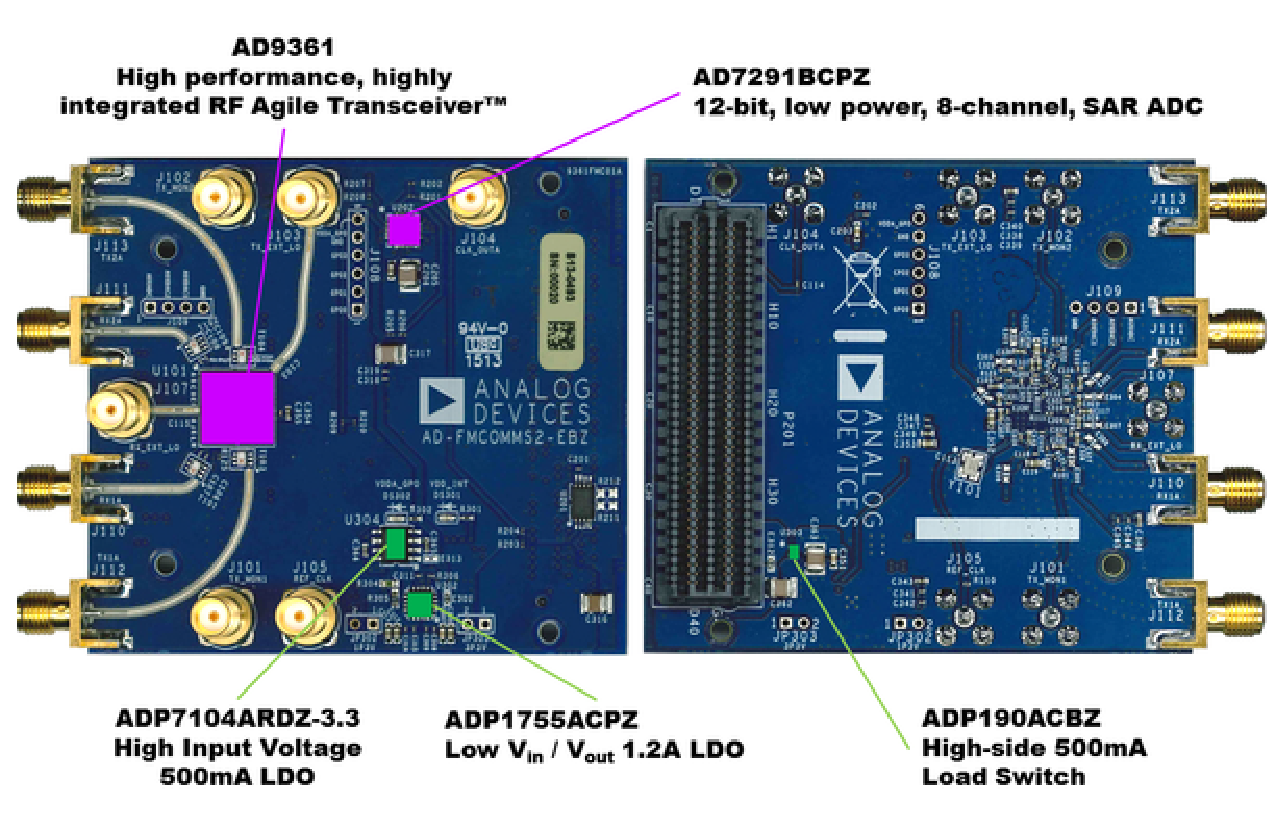
\includegraphics[width=0.65\textwidth]{./figures/fmcomms2_pic}
    \caption{ FMComms2 and its components
    \label{fig:fmcomm}}
\end{figure}

\subsection{Control Interface}

As stated in the previous subsection the FMComms2 control and communication
interface is implemented through GPIO pins and SPI protocol, basically SPI is
used to write and read registers in the board while GPIO is used for real-time
control, like reset or change states in the ENSM.\\

While the development was in its beginning the minimum pins for communication
and reset work were assigned, however when the development wen to Vivado with
the VC707 there was the need to build something more automated in order to be
easily rebuild, so the \emph{ad9361\_comm} IP was created to route the respective
pins from SPI and GPIO interfaces to the ad9361 control and communication interface.\\

Below it is possible to see in a simple schematic what is the \emph{ad9361\_comm}
IP and how it routes the respective ports to the ad9361 interface.

%diagrama de blocos control interface
\begin{figure}[htbp]
    \centering
    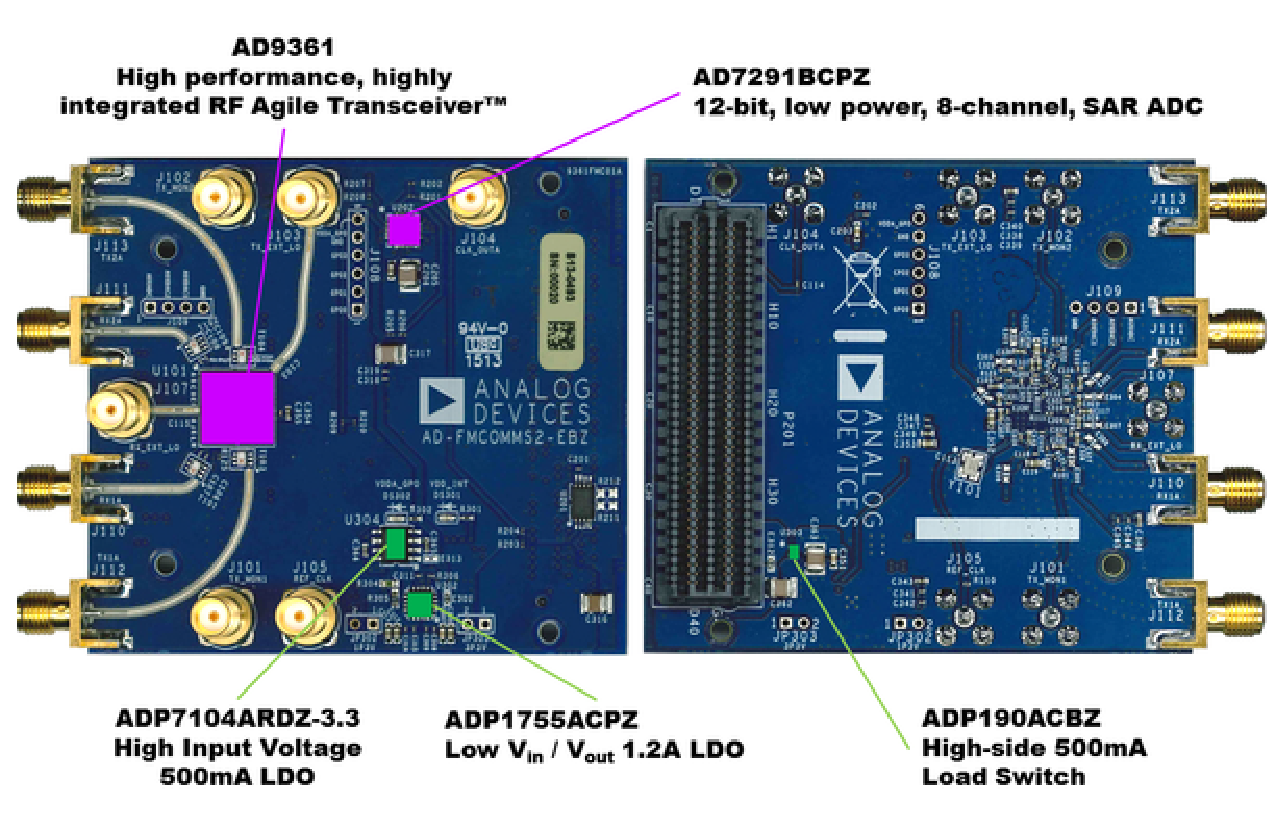
\includegraphics[width=0.65\textwidth]{./figures/fmcomms2_pic}
    \caption{ FMComms2 and its components
    \label{fig:fmcomm}}
\end{figure}

\subsection{Transmitting custom data}

After having the communication and initialization between FPGA and FMComms2 board
working properly, the next step was to input custom data into the device and
efficiently transmit modulated information in the carrier wave.

There is two basic ways to input data into the AD9361, to do so it is necessary to understand
its communication interface, which is similar to the axi-stream interface with
3 ports, one for data, one for enable and one for valid. The first approach for
input data into the transceiver was use a FIFO with a DDS IP in the fpga, which
is not so fast and reliable, but worked for test purposes.

%inserir figura do IP ad9361 highlight TX interface pins
\begin{figure}[htbp]
    \centering
    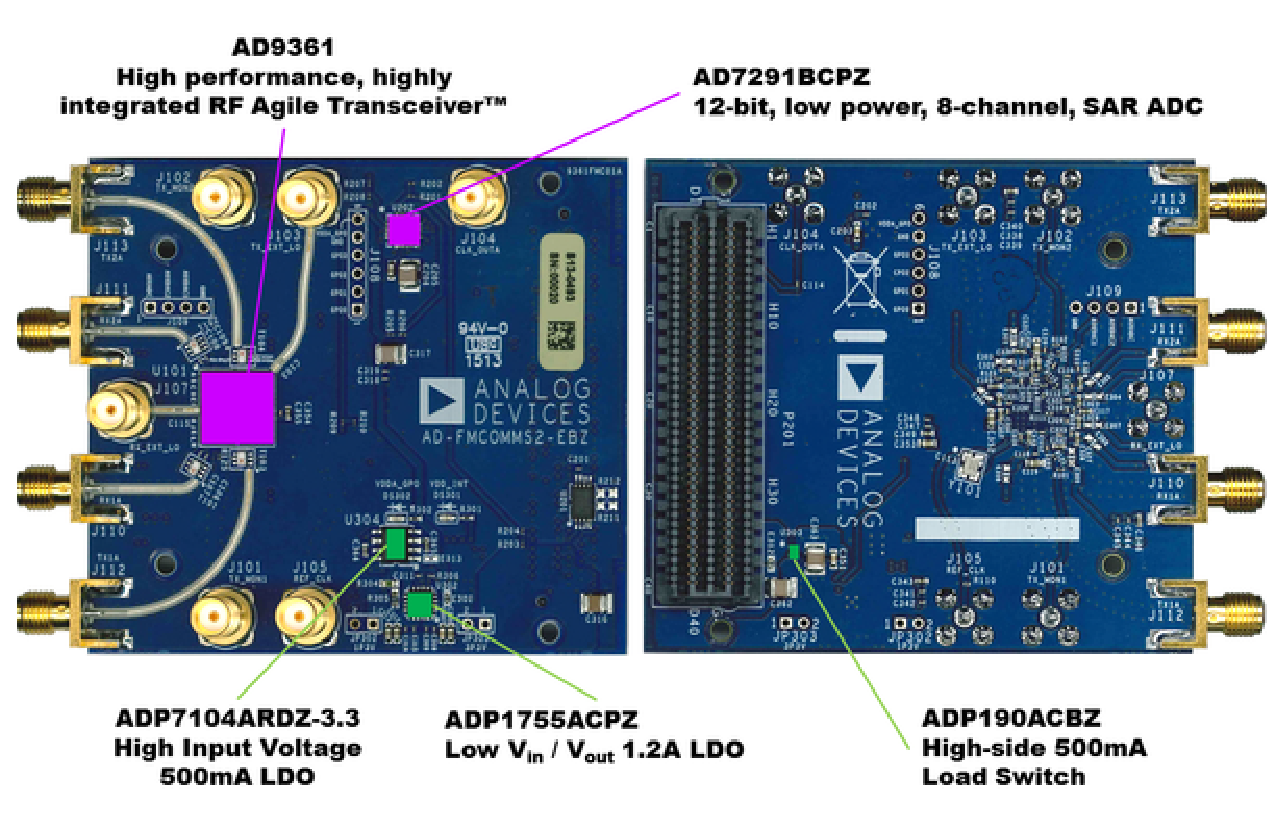
\includegraphics[width=0.65\textwidth]{./figures/fmcomms2_pic}
    \caption{ FMComms2 and its components
    \label{fig:fmcomm}}
\end{figure}

%inserir diagrama de blocos de entrada DDS>FIFO>AD9361

\begin{figure}[htbp]
    \centering
    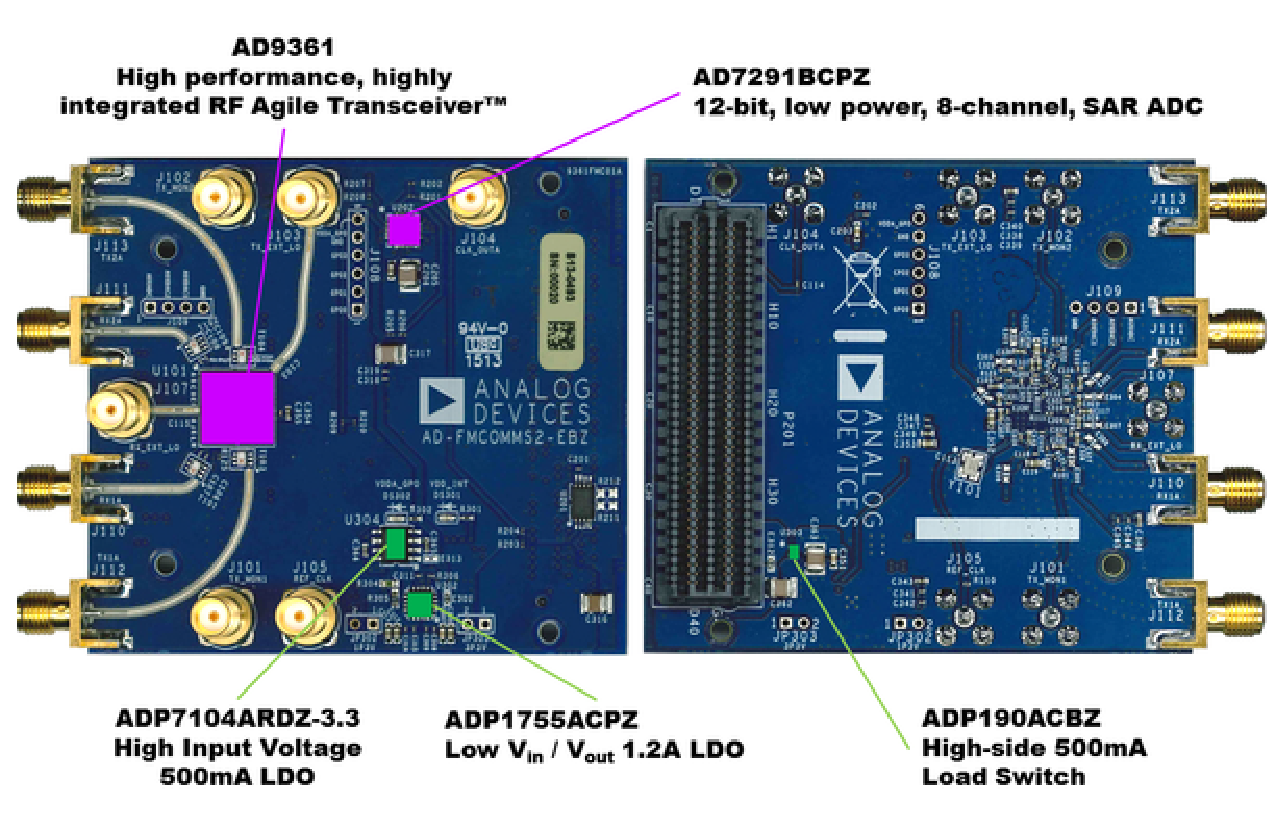
\includegraphics[width=0.65\textwidth]{./figures/fmcomms2_pic}
    \caption{ FMComms2 and its components
    \label{fig:fmcomm}}
\end{figure}

After some time, the need for a faster interface rose, then the use of DMA came
naturally, because it is faster and more reliable than the common FIFO.

%inserir figura da interface DMA>AD9361
\begin{figure}[htbp]
    \centering
    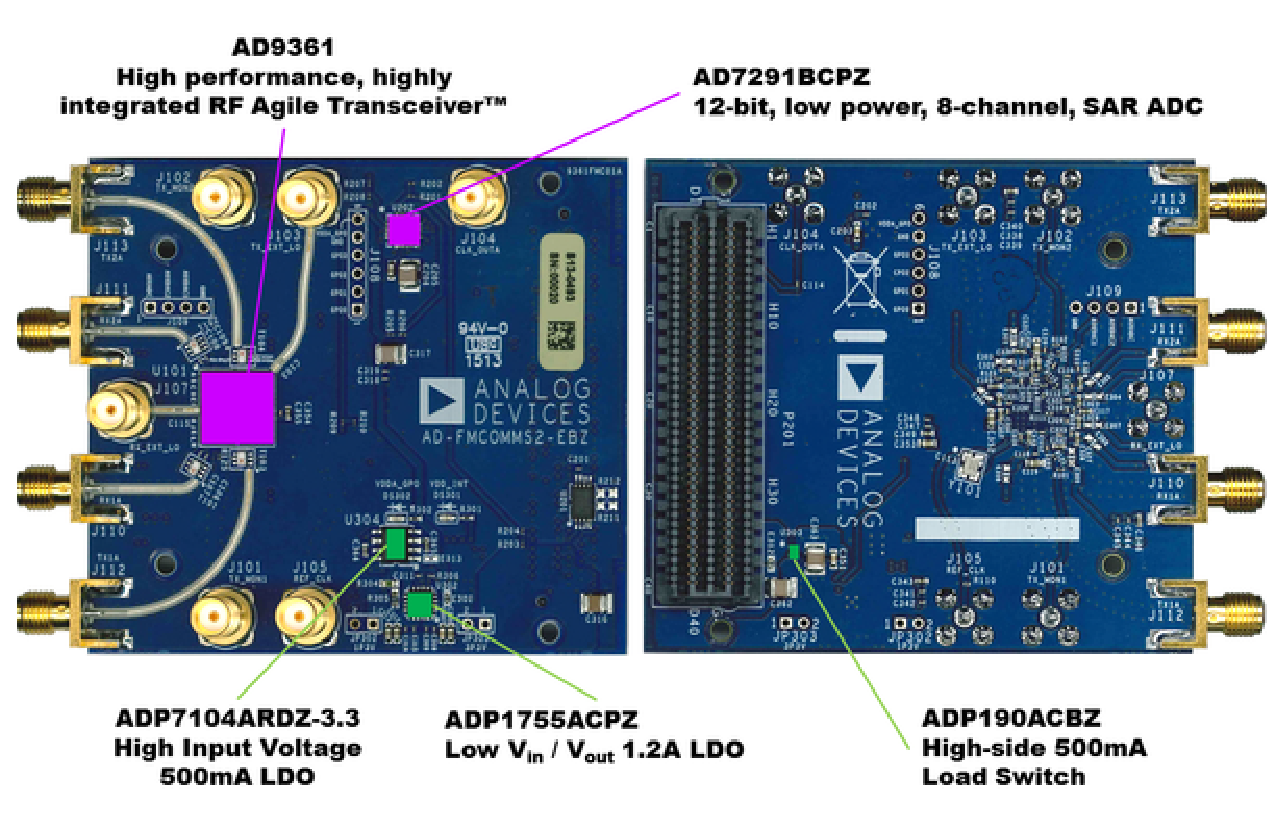
\includegraphics[width=0.65\textwidth]{./figures/fmcomms2_pic}
    \caption{ FMComms2 and its components
    \label{fig:fmcomm}}
\end{figure}

\subsection{Receiving Custom data}

Receiving is the exact opposite of transmitting custom data, in the beginning of
the setup implementation using a DDS IP and a fifo to input IQ data into the
AD9361 was intuitively the easier way for transmission, and indeed was the same
thing for receiving.

%inserir figura do IP ad9361 Highlight RX interface pins
\begin{figure}[htbp]
    \centering
    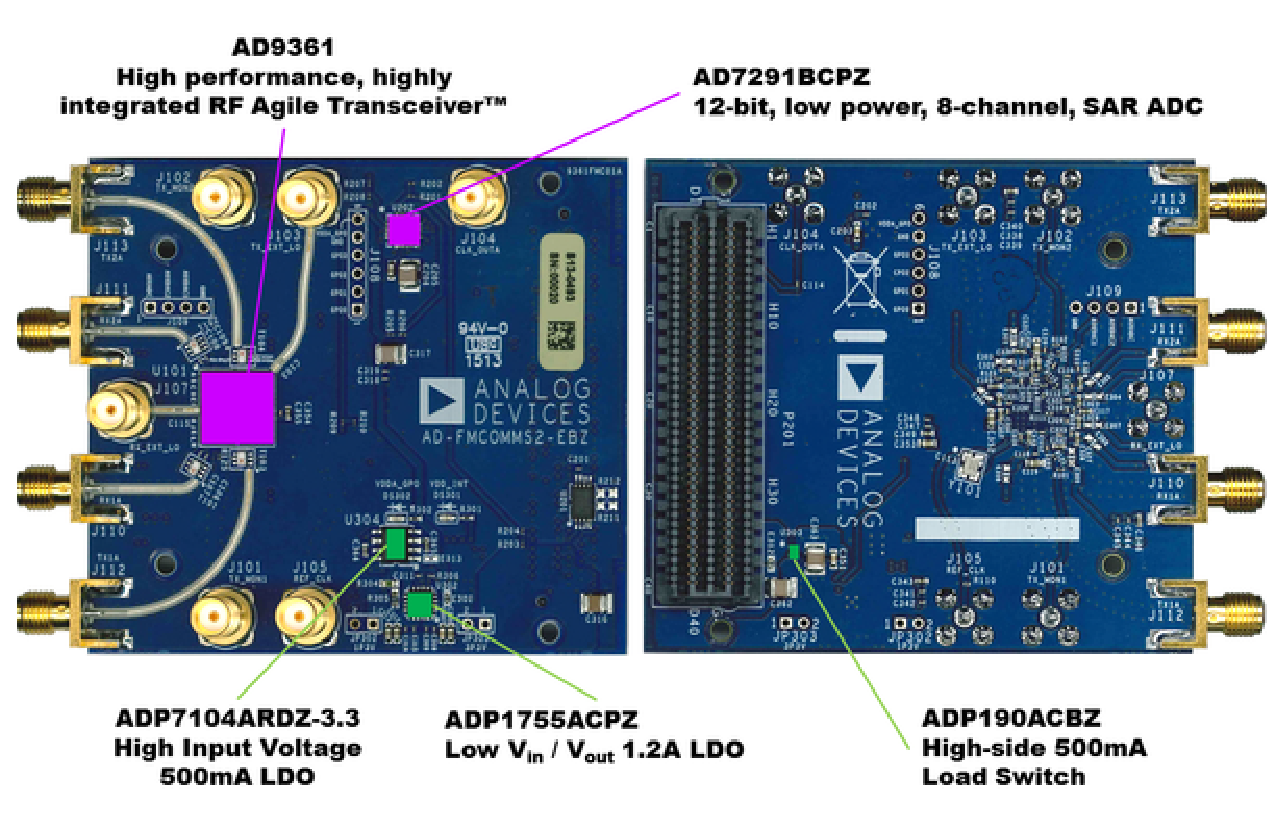
\includegraphics[width=0.65\textwidth]{./figures/fmcomms2_pic}
    \caption{ FMComms2 and its components
    \label{fig:fmcomm}}
\end{figure}

%inserir diagrama de blocos de entrada AD9361>FIFO>ILA
\begin{figure}[htbp]
    \centering
    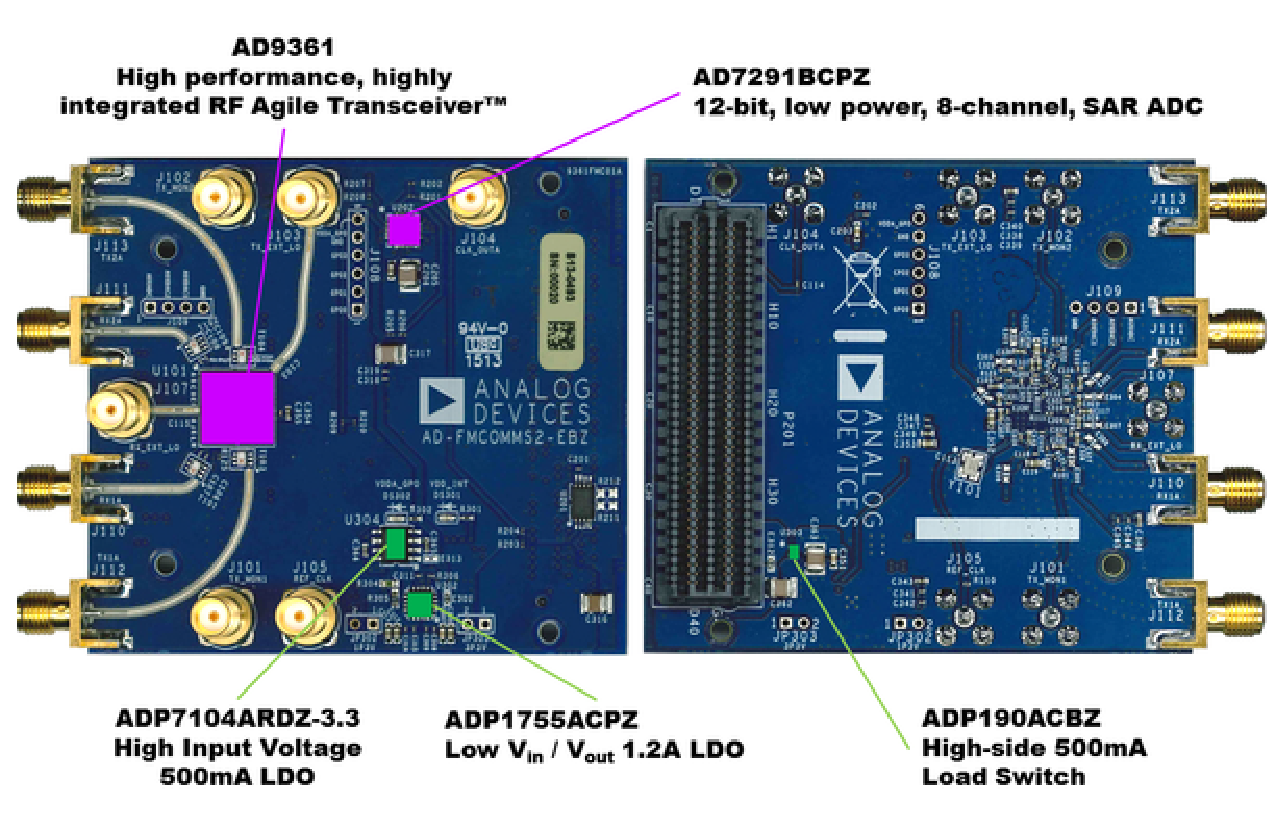
\includegraphics[width=0.65\textwidth]{./figures/fmcomms2_pic}
    \caption{ FMComms2 and its components
    \label{fig:fmcomm}}
\end{figure}

The same idea used in transmission when the VC707 development began was applied
to the receiver, use DMA.

%inserir figura da interface AD9361>DMA
\begin{figure}[htbp]
    \centering
    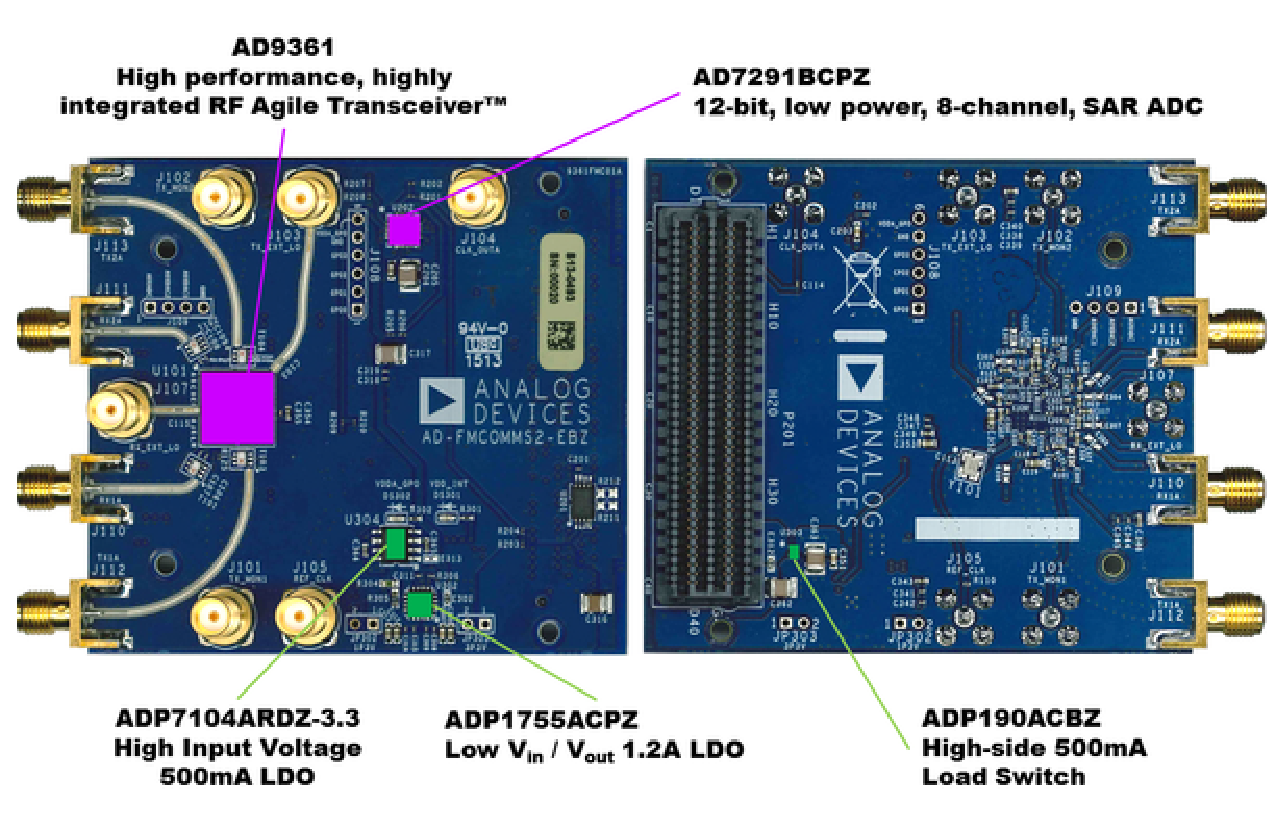
\includegraphics[width=0.65\textwidth]{./figures/fmcomms2_pic}
    \caption{ FMComms2 and its components
    \label{fig:fmcomm}}
\end{figure}

\subsection{Data Interface}
After various experimentations in data transmission, the data interface with the
DAC and ADC was planned,

%ad9361_data interface image
\begin{figure}[htbp]
    \centering
    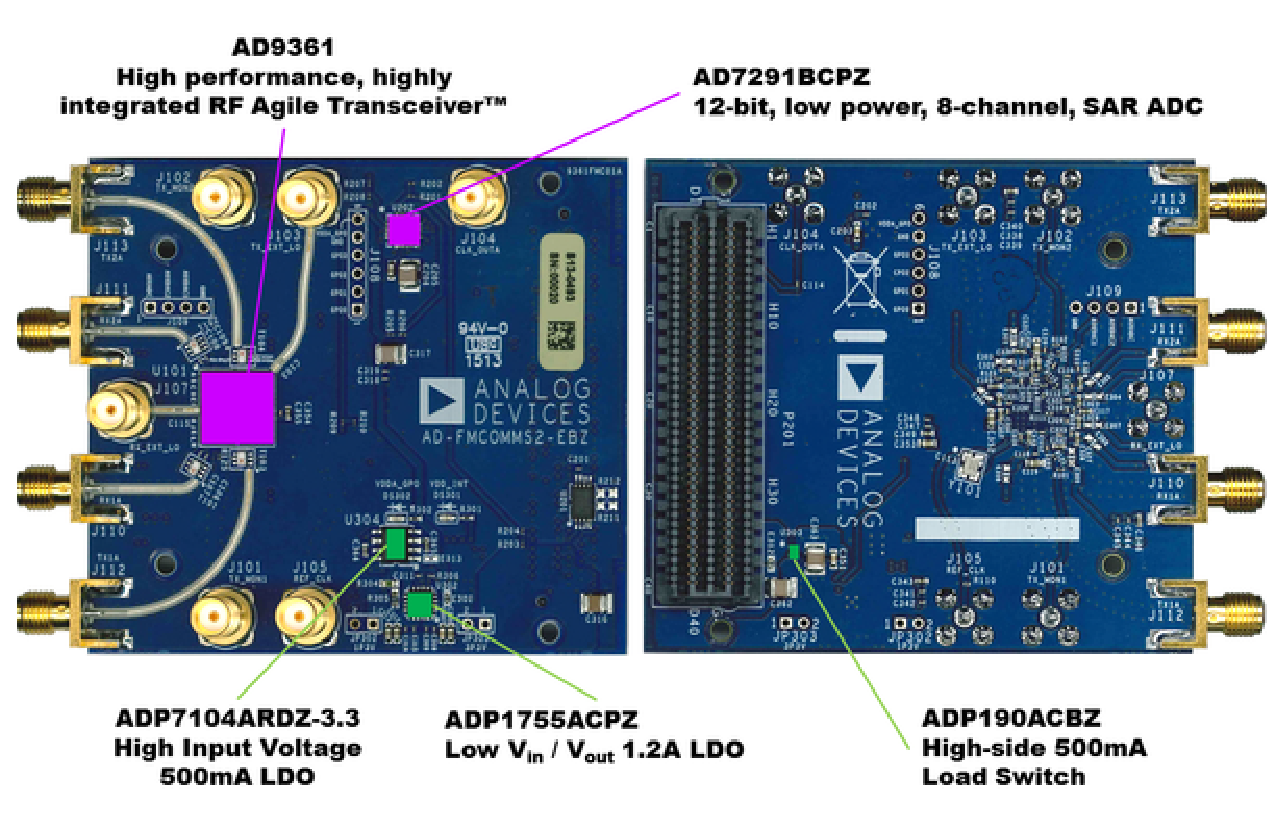
\includegraphics[width=0.65\textwidth]{./figures/fmcomms2_pic}
    \caption{ FMComms2 and its components
    \label{fig:fmcomm}}
\end{figure}

\section{Driver}



\section{Applications}


\part{Final Results}
\chapter{Results}
\label{chap:results}

This works goals were divided in basically three steps, configuration, transmission
and reception, having these three steps barely working it is possible to make a
transmission and analyze data. It is possible to see in figure \ref{fig:setup}
how the hardware is arranged and in figure \ref{fig:setupbd} it is possible to
behold the setup's block diagram, which gives the idea of the complexity behind
the design and how each component is connected.

%foto setup pronto
\begin{figure}[htbp]
    \centering
    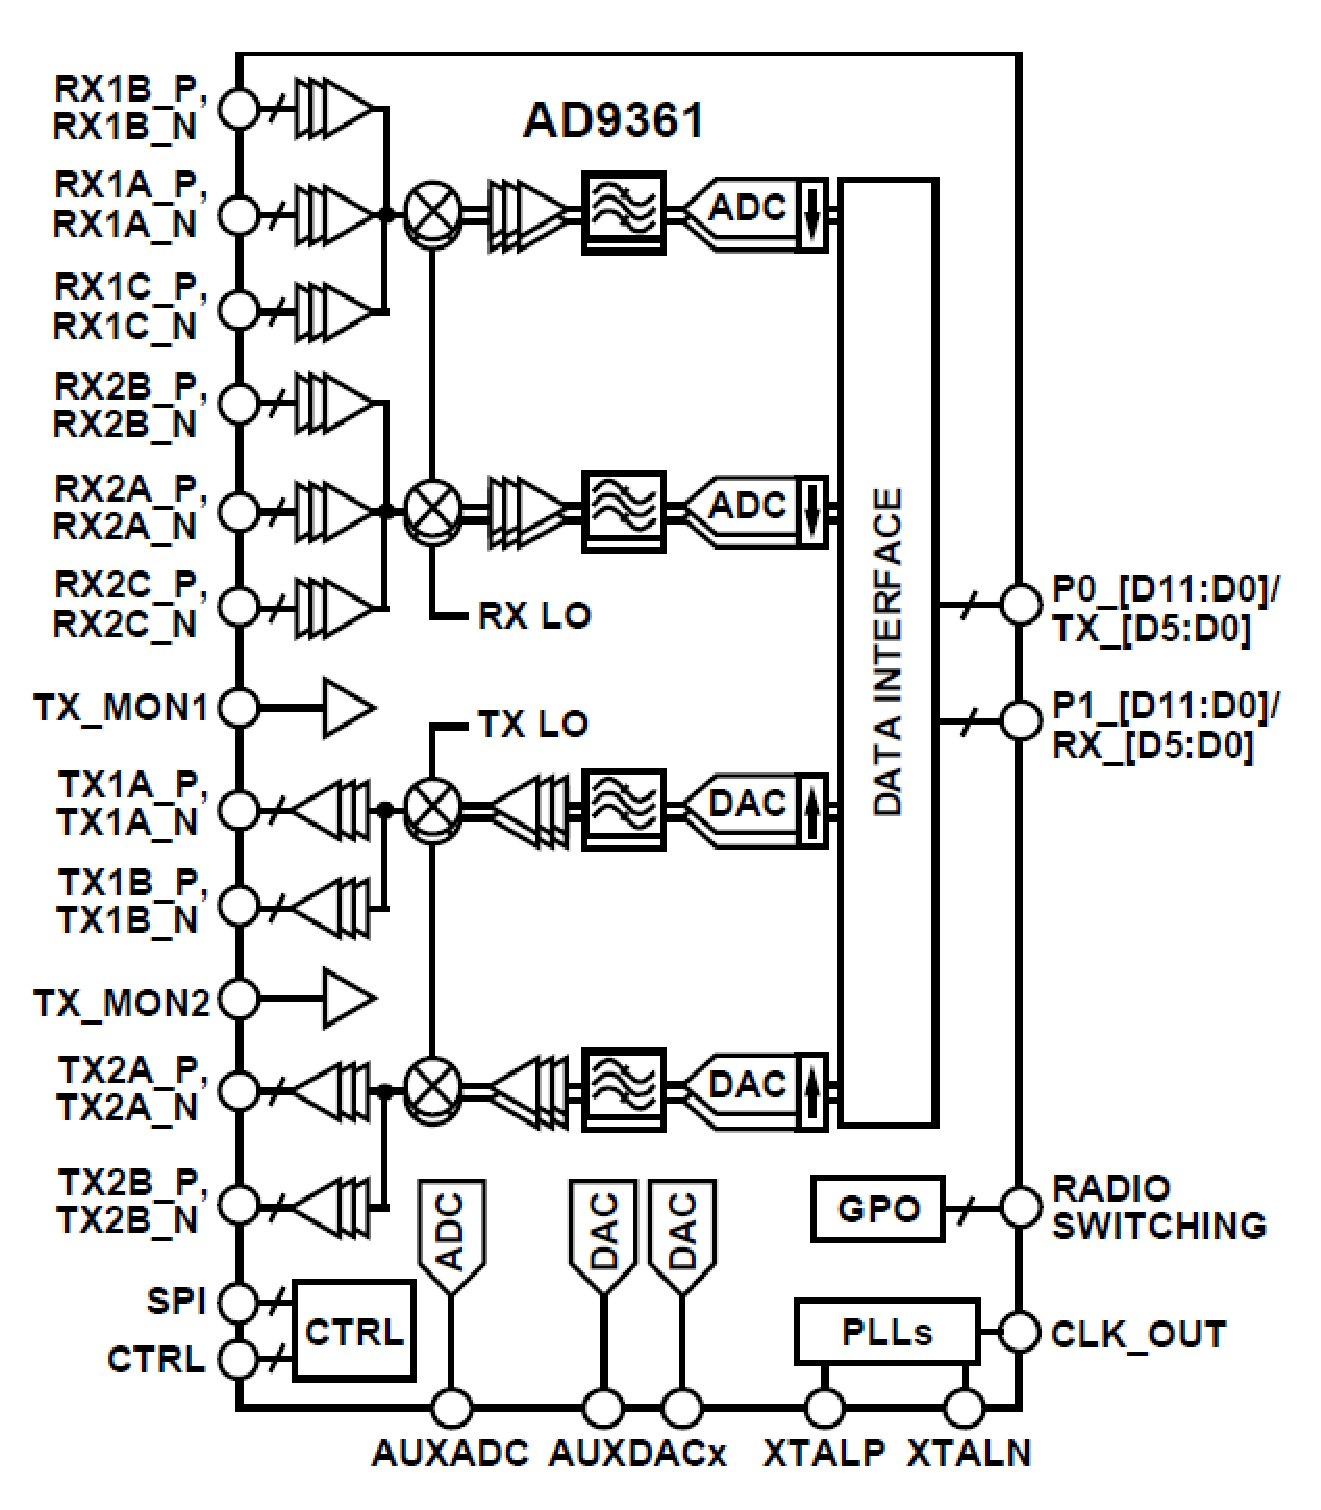
\includegraphics[width=0.45\textwidth]{./figures/ad9361_functional_diagram}
    \caption{ Image of the Setup Hardware
    \label{fig:setup}}
\end{figure}

\begin{figure}[htbp]
    \centering
    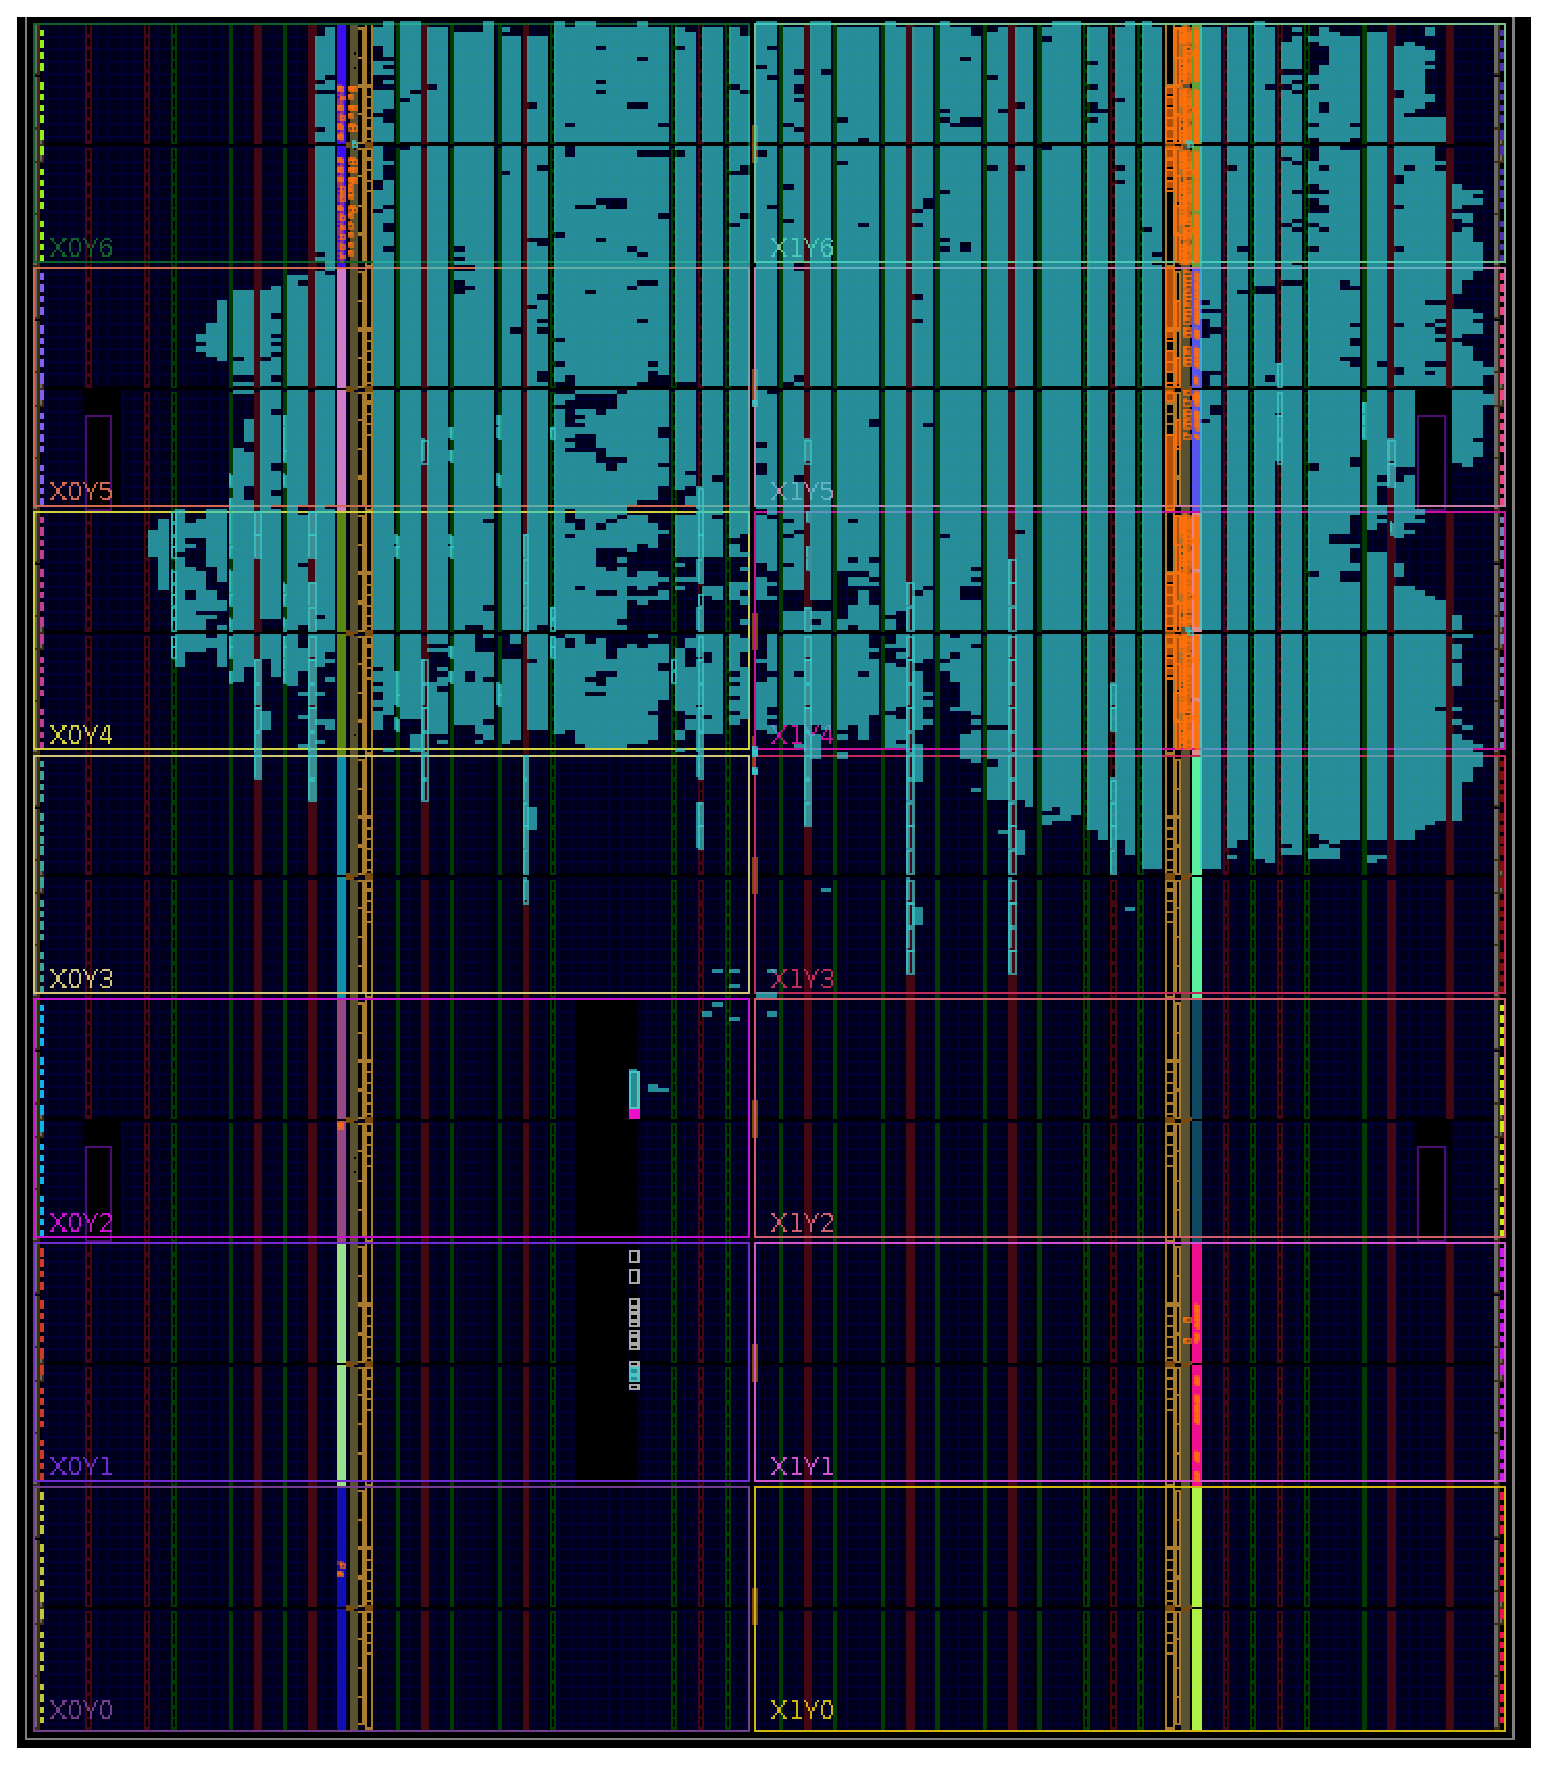
\includegraphics[width=0.35\textwidth]{./figures/fpga_area}
    \caption{ FPGA area used in this Setup
    \label{fig:fpgaarea}}
\end{figure}

%foto diagrama de blocos
\begin{figure}[htbp]
    \centering
    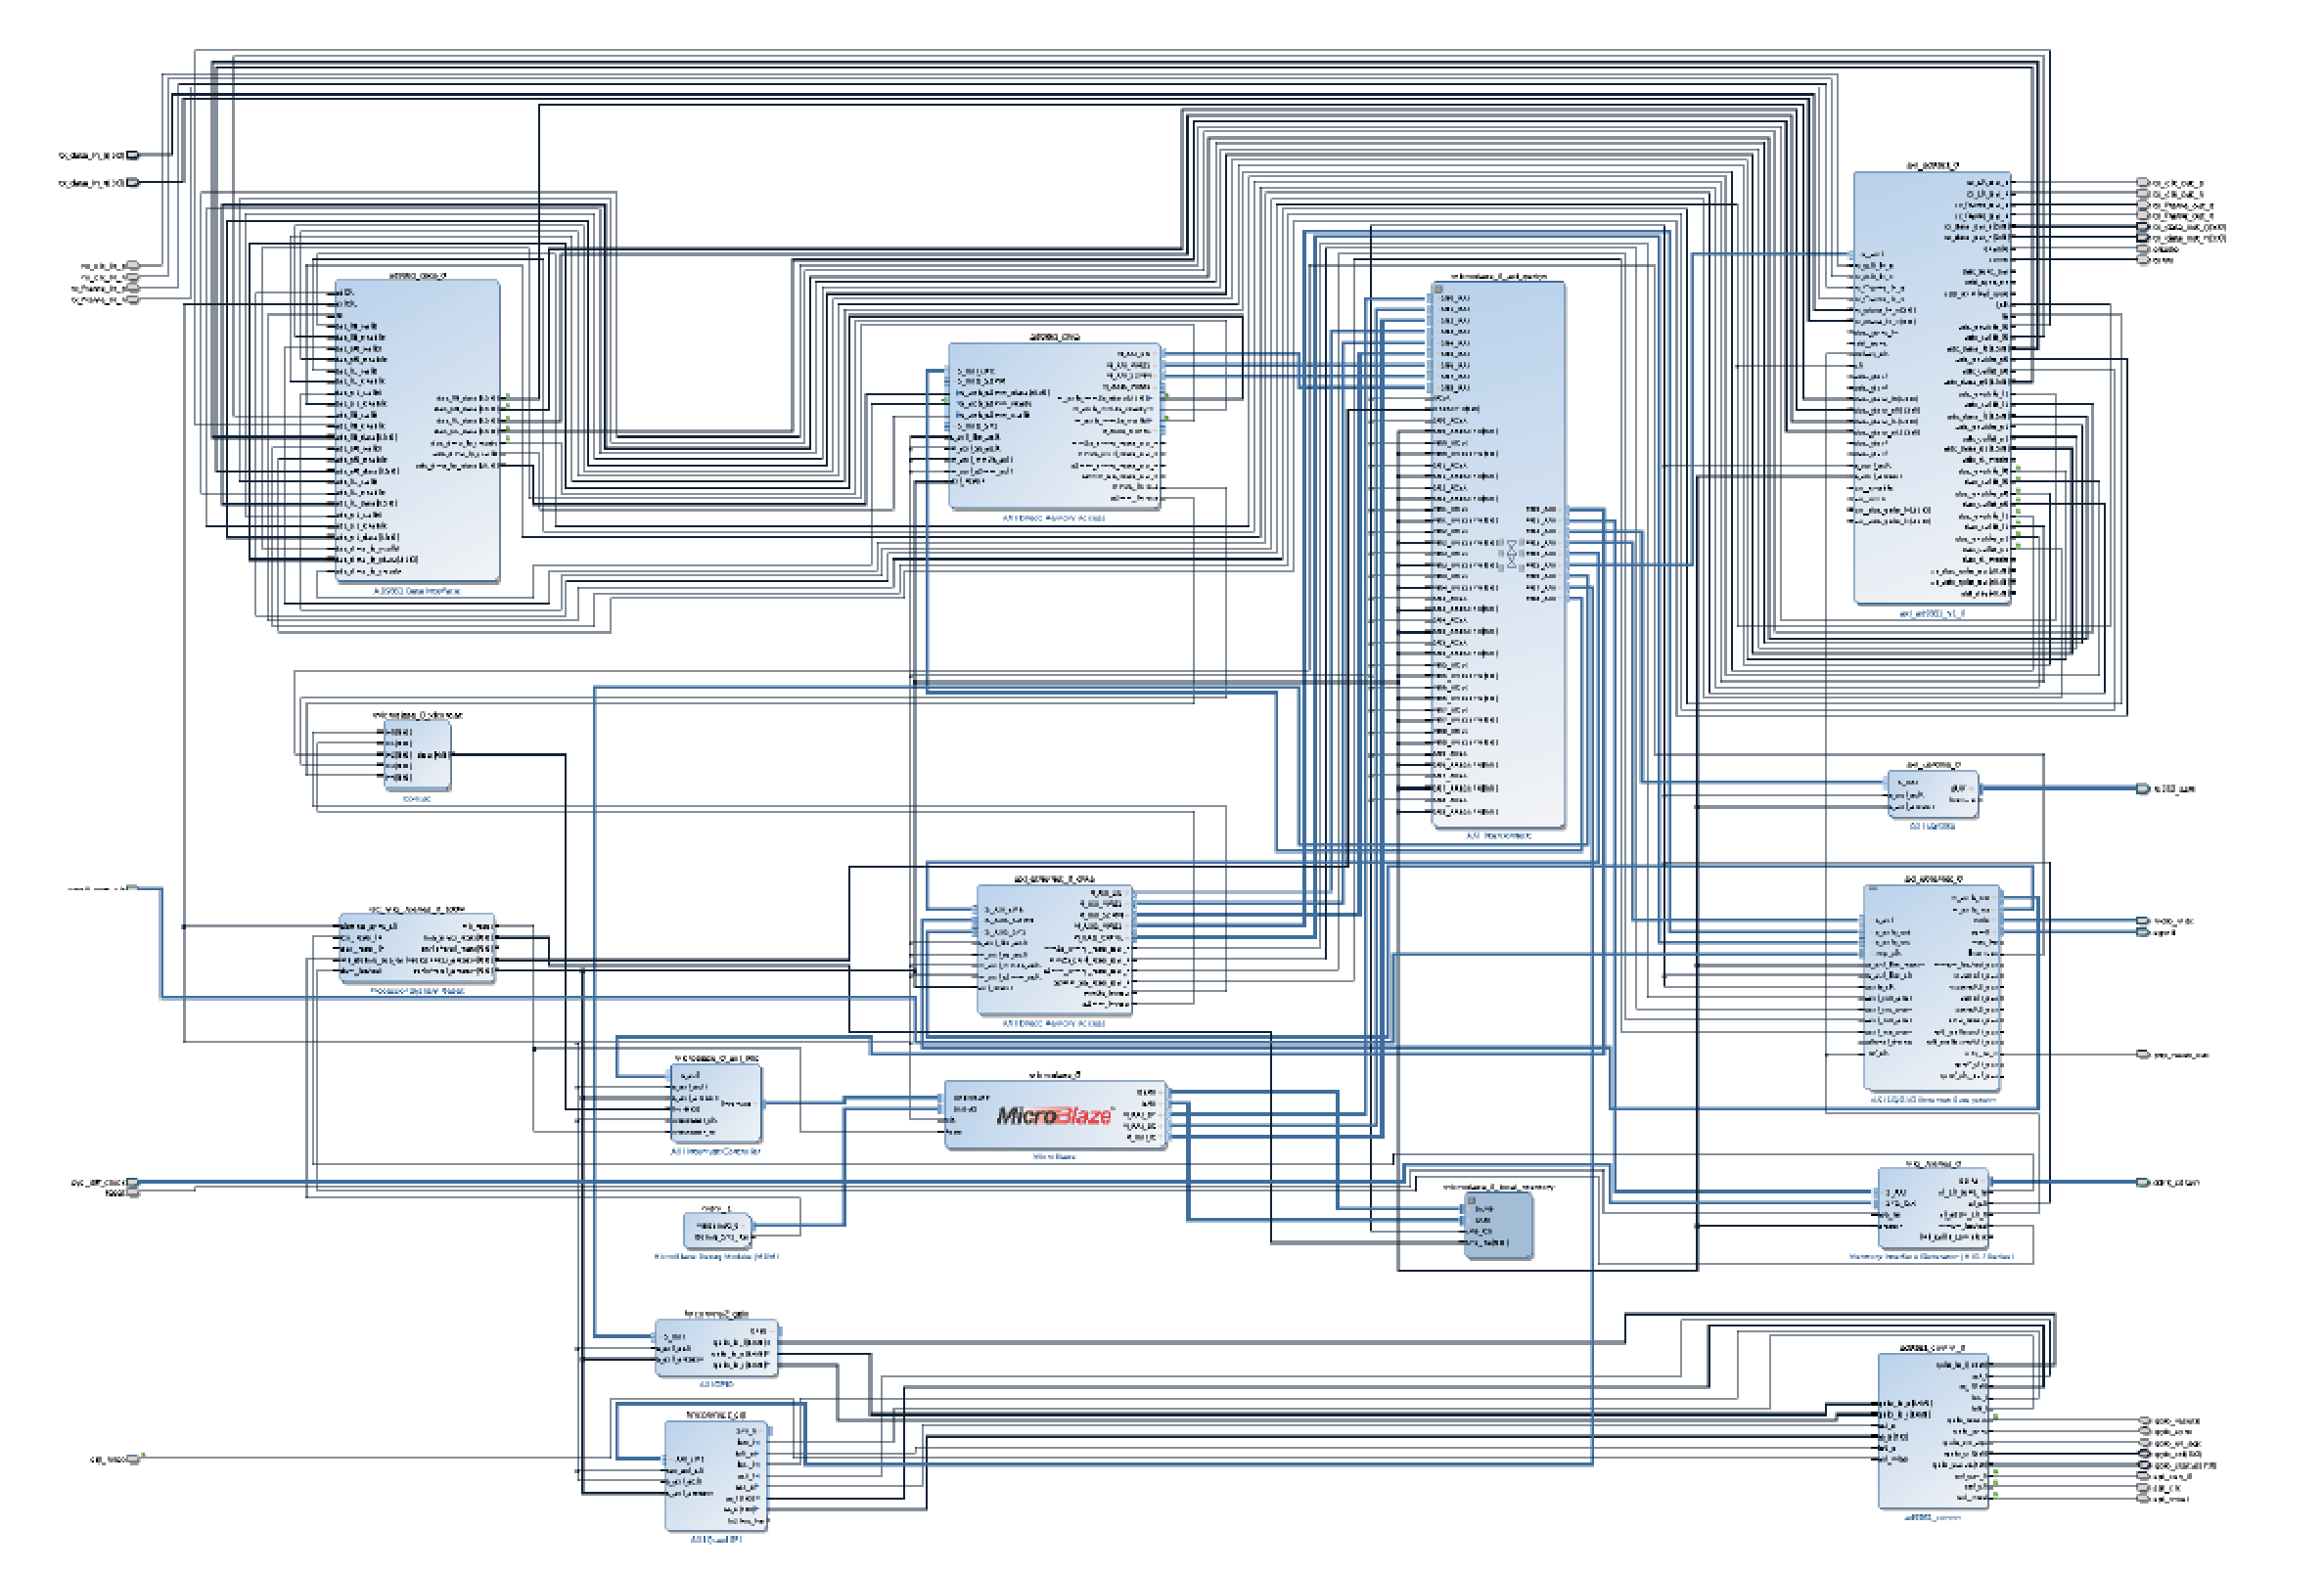
\includegraphics[width=0.95\textwidth]{./figures/setup_bd}
    \caption{ Image of the Setup Block diagram
    \label{fig:setupbd}}
\end{figure}

\vfill
\clearpage

\section{Preliminary Tests}
\label{result:conf}

The preliminary tests were focusing on initializing and communication between FPGA
and the FMComms2 board, in the previous chapter the steps of setting up communication
and control interface were described, and it describes also how this interface works
and how a block was made to implement such, in short it was needed to set up SPI and GPIO
modules and make the right input and output ports specified in \ref{subs:controlif} and
after the initialization and callibration is finished, it is possible to observ the
carrier wave centralized at the frequency 2.4 Ghz.

To generate the outputs two analyzers were used, one oscilloscope and one spectrum analyzer,
both analyzers outputs can be seen in the figures below:

%spectrum analyser image
\begin{figure}[htbp]
    \centering
    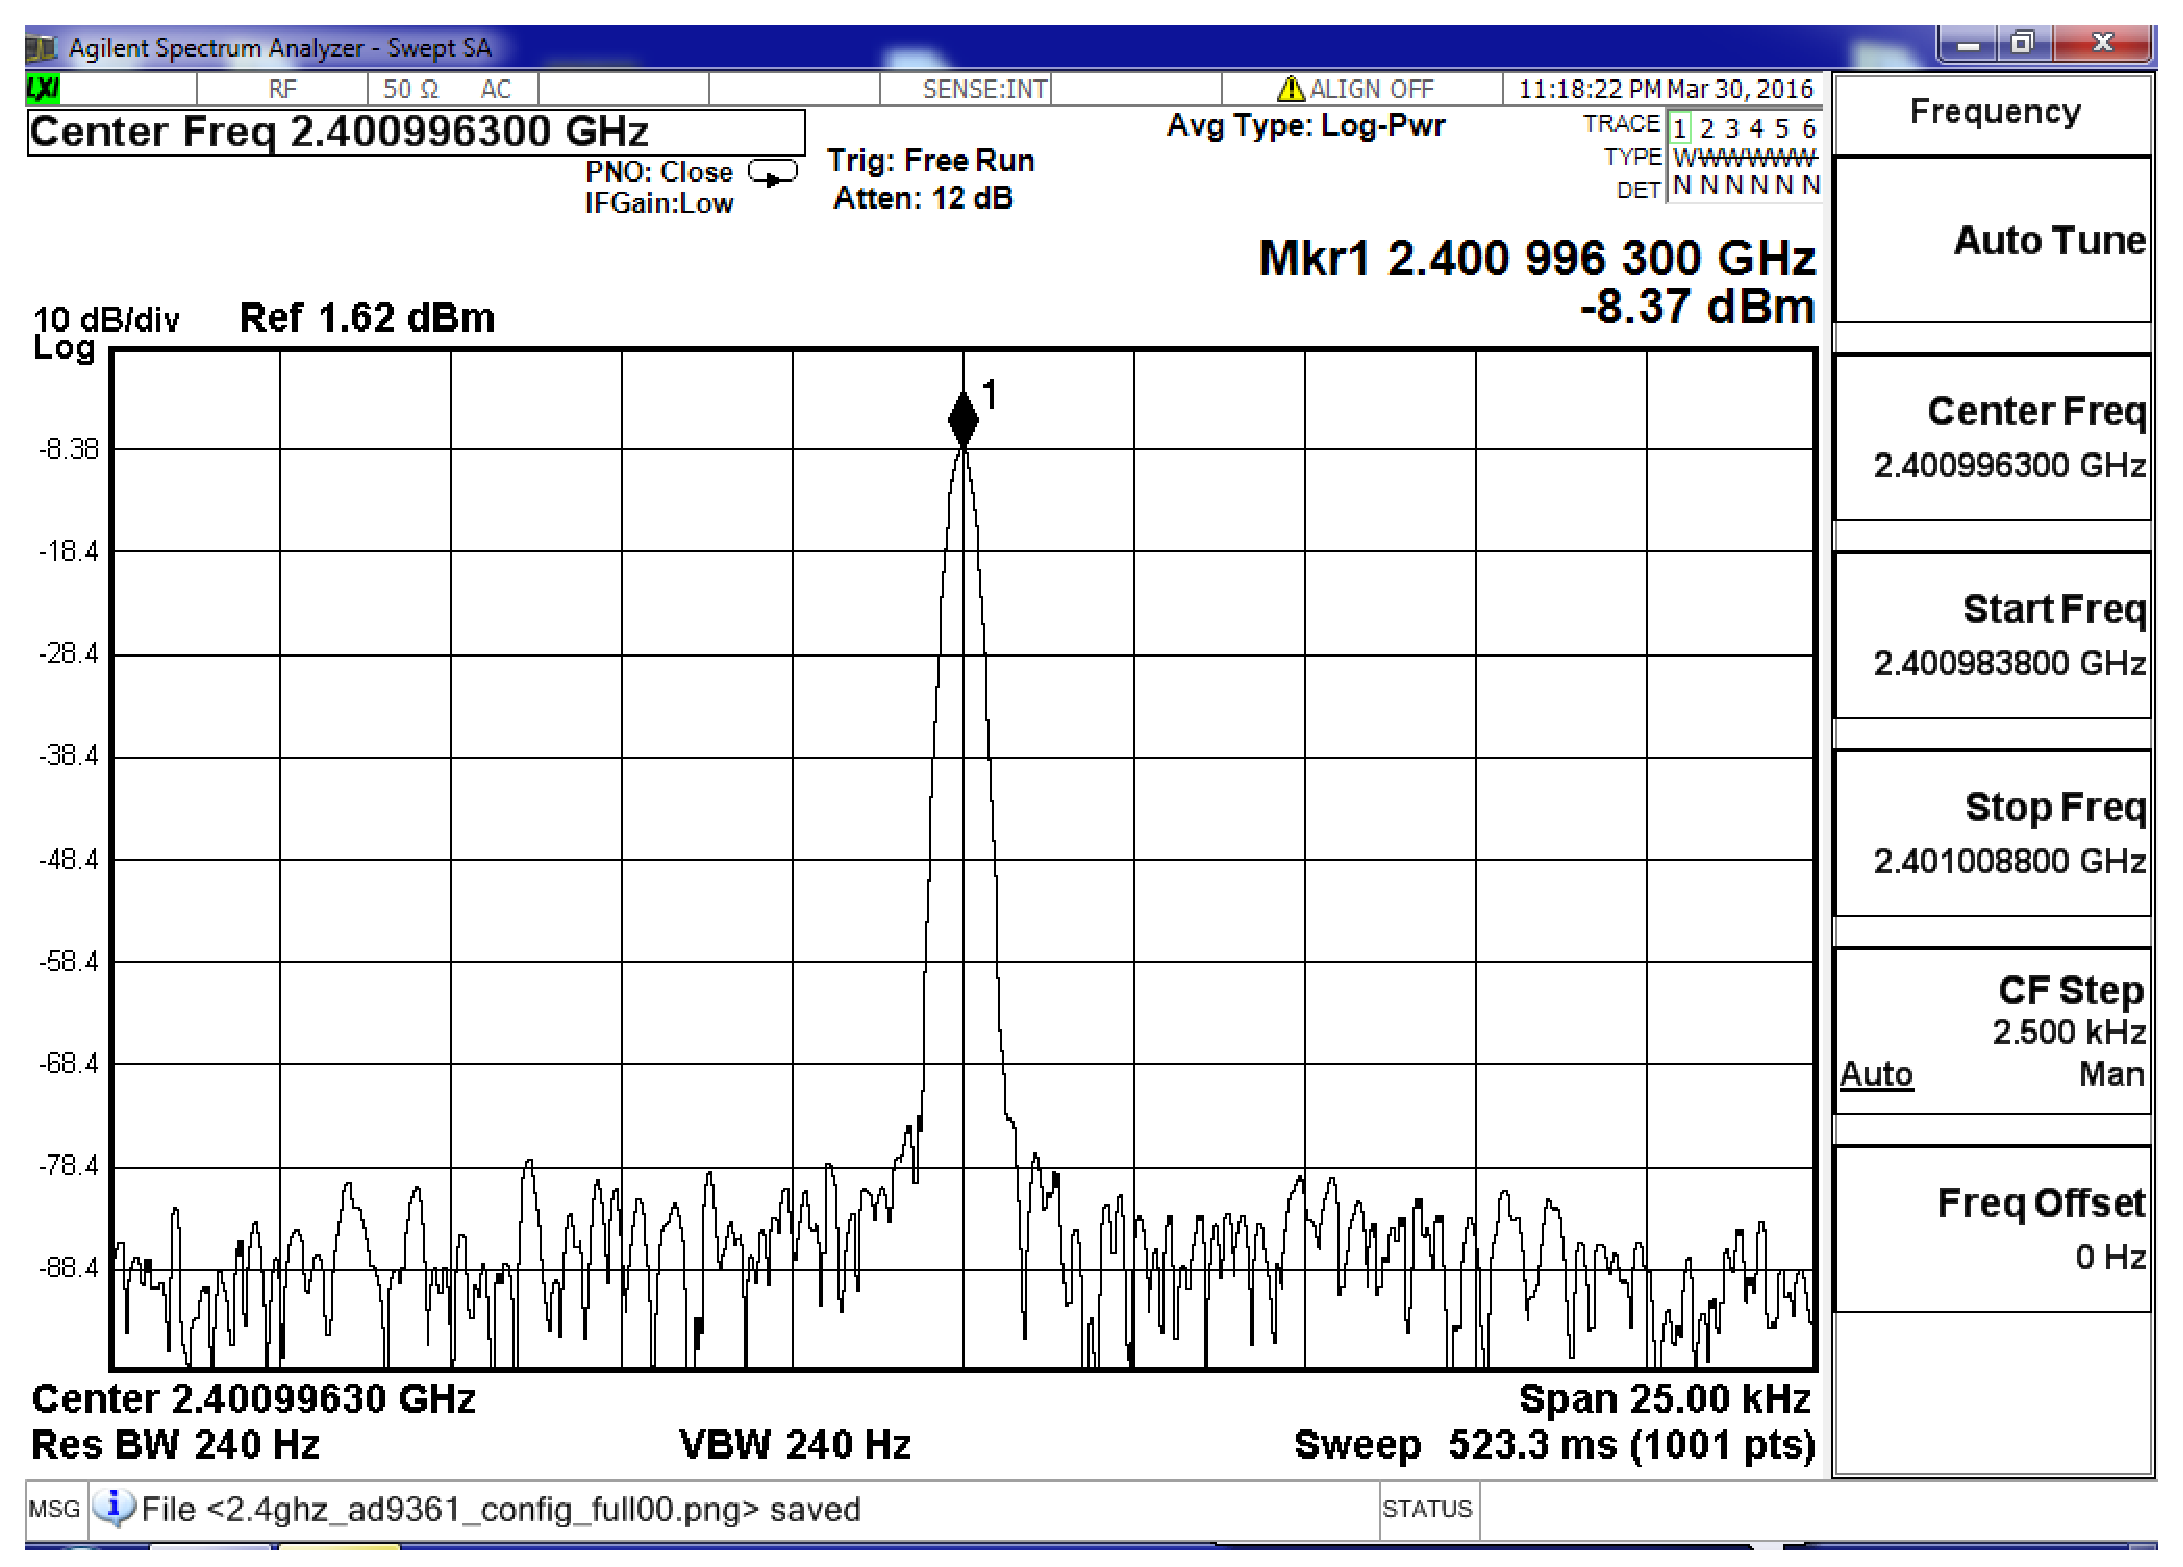
\includegraphics[width=0.85\textwidth]{./figures/spectrum_init}
    \caption{ Spectrum Analyzer Screen
    \label{fig:spec}}
\end{figure}

%initialization
\begin{figure}[htbp]
    \centering
    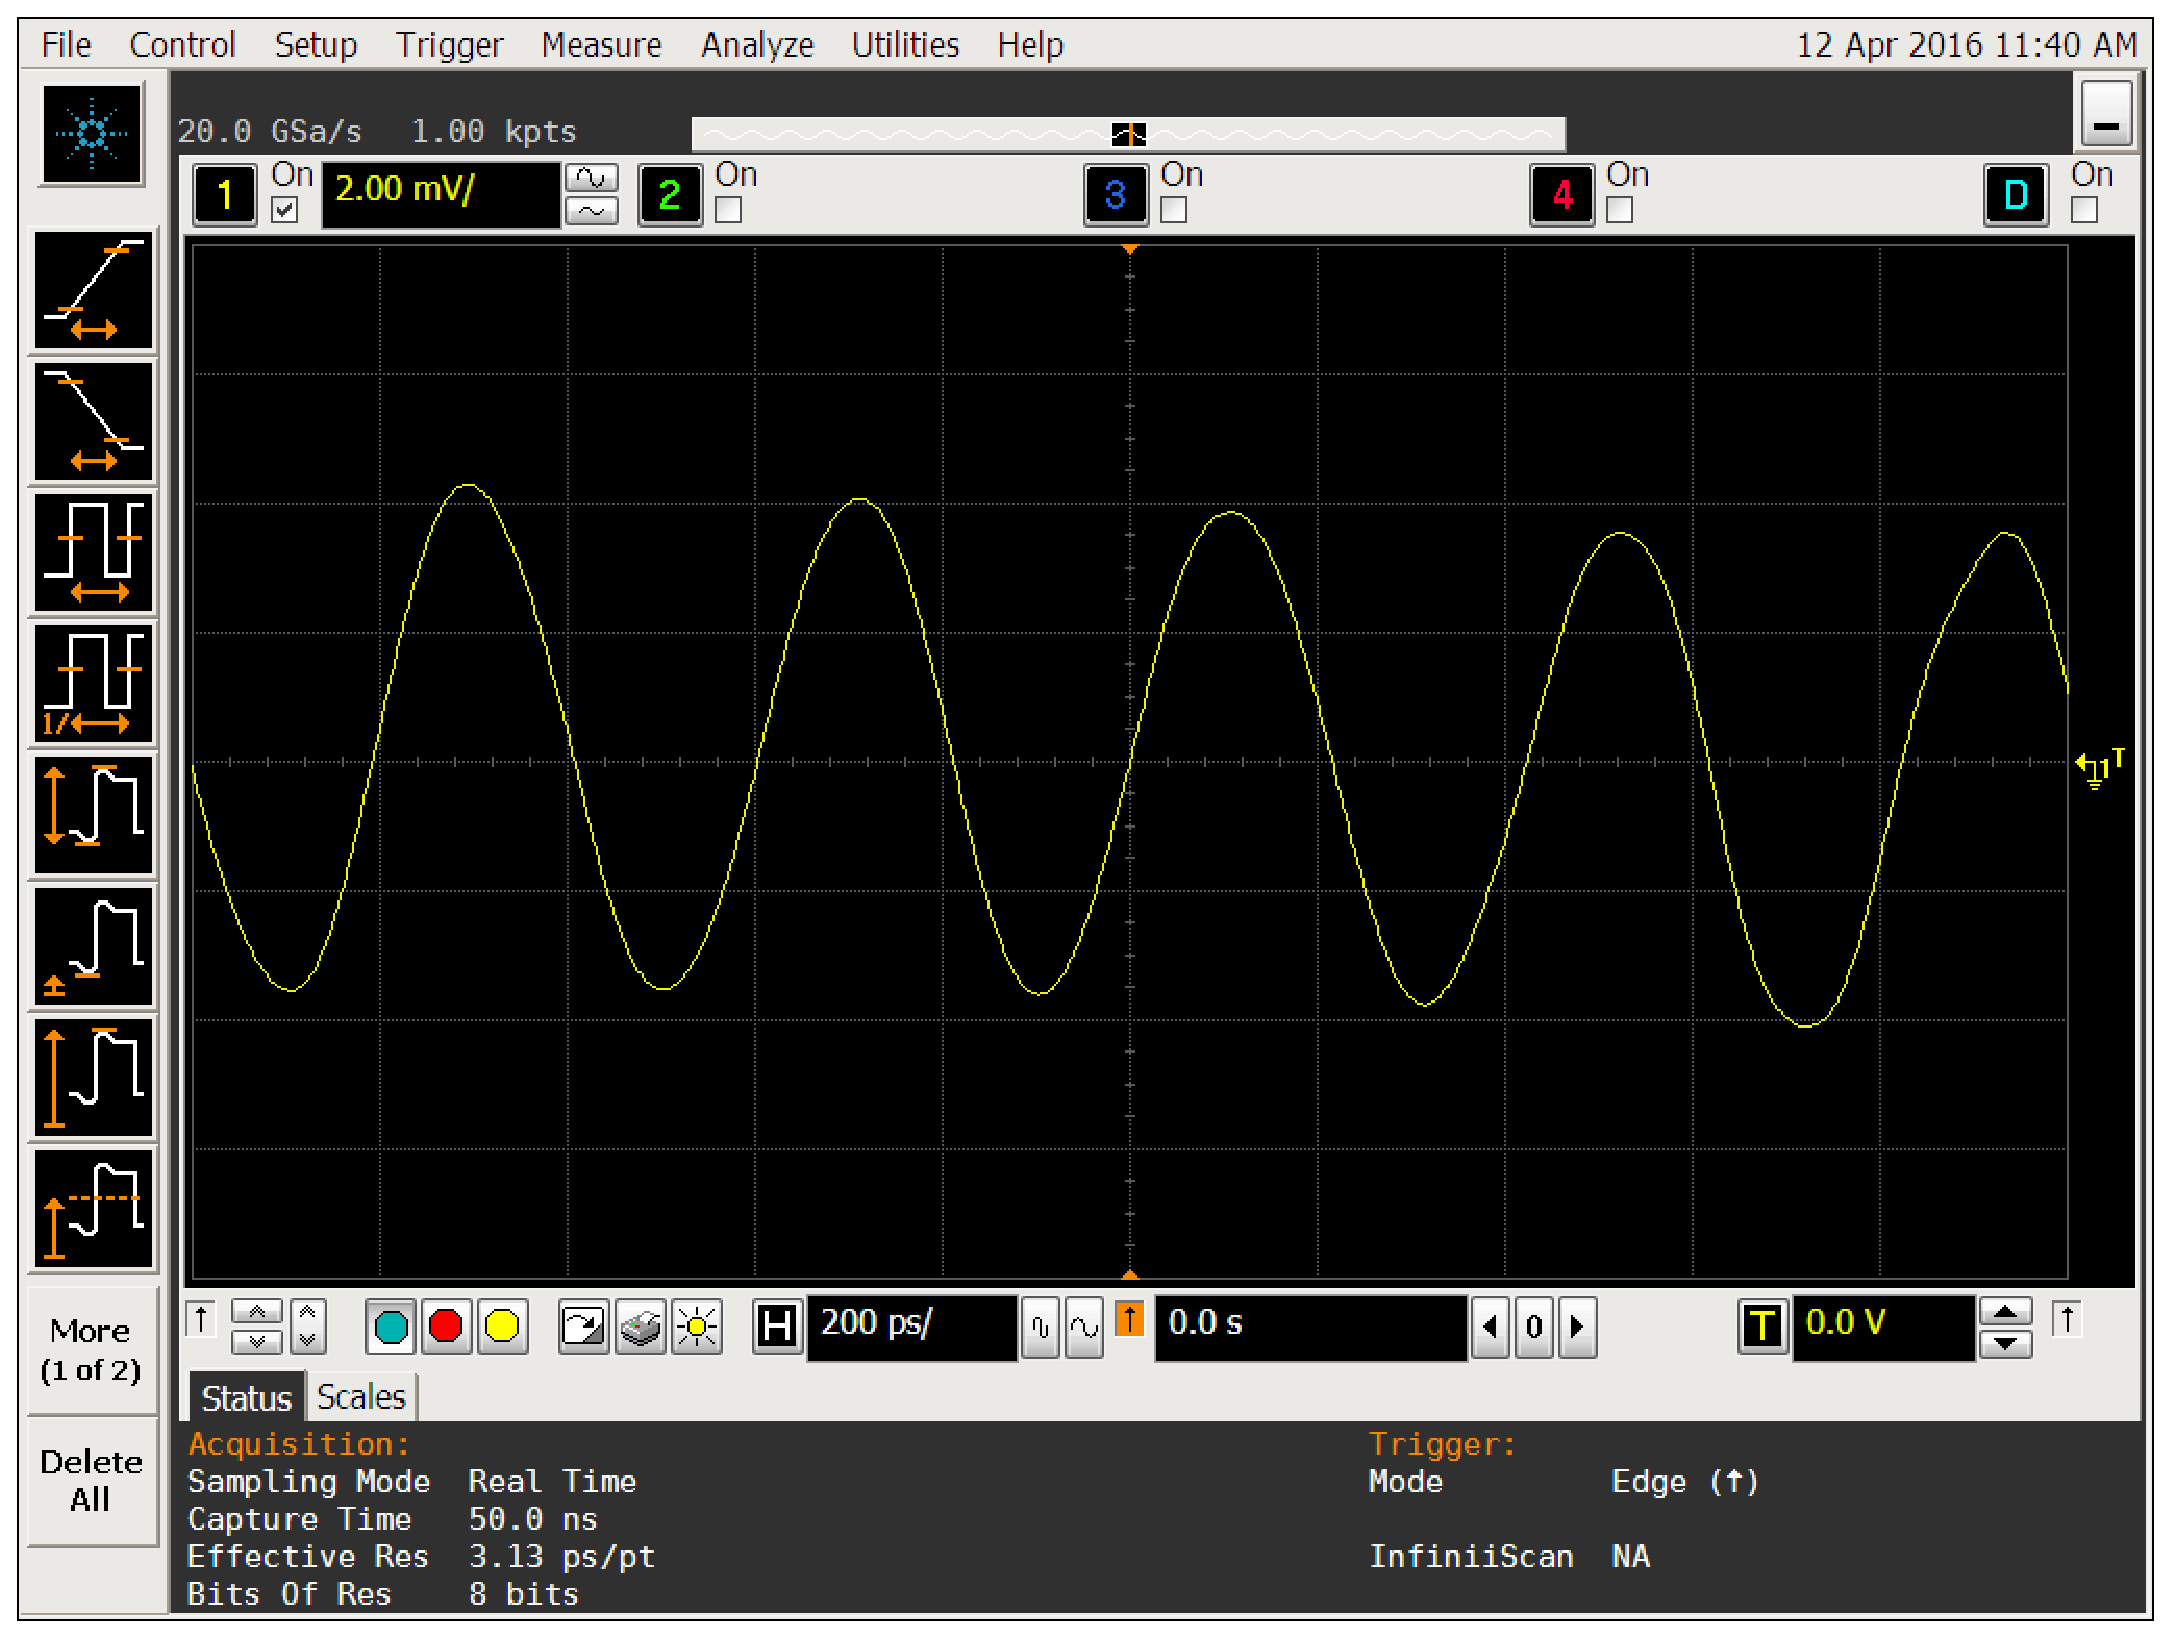
\includegraphics[width=0.85\textwidth]{./figures/oscill_init}
    \caption{ Carrier Waveform after Initialization
    \label{fig:oscillinit}}
\end{figure}

%digital tune
\begin{figure}[htbp]
    \centering
    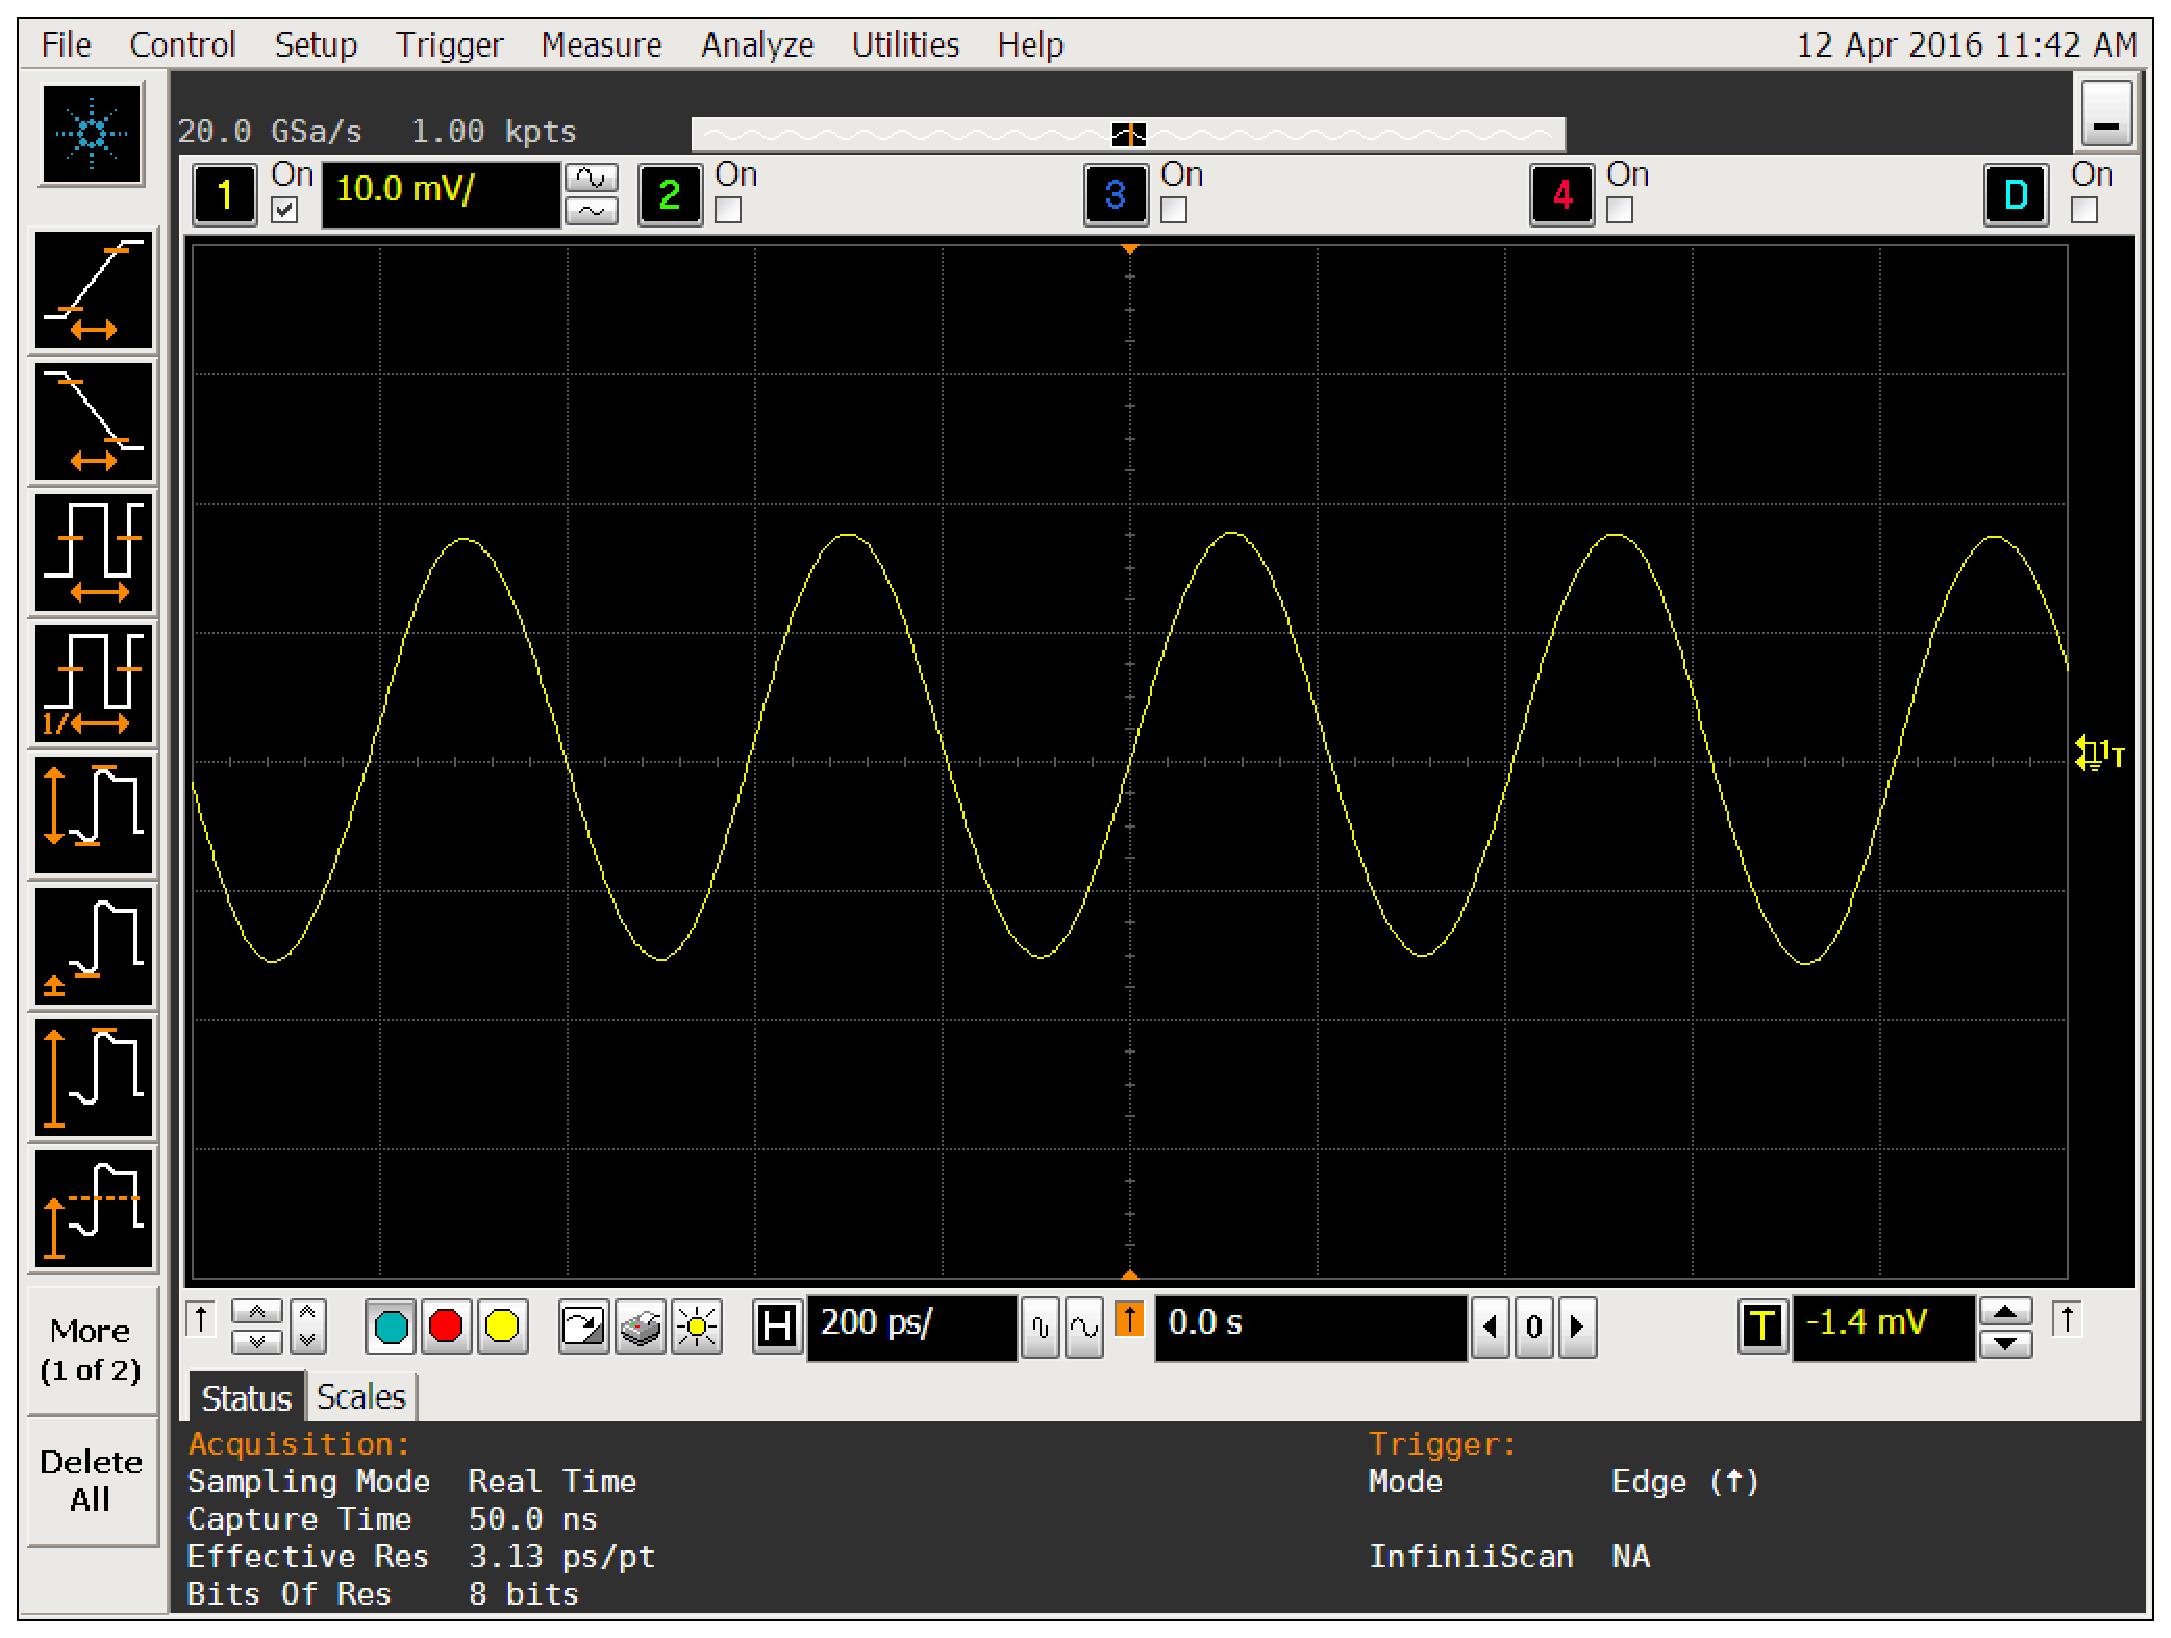
\includegraphics[width=0.85\textwidth]{./figures/oscill_dig}
    \caption{ Carrier Waveform after Tunning Digital Interface
    \label{fig:oscilldig}}
\end{figure}

%freq
\begin{figure}[htbp]
    \centering
    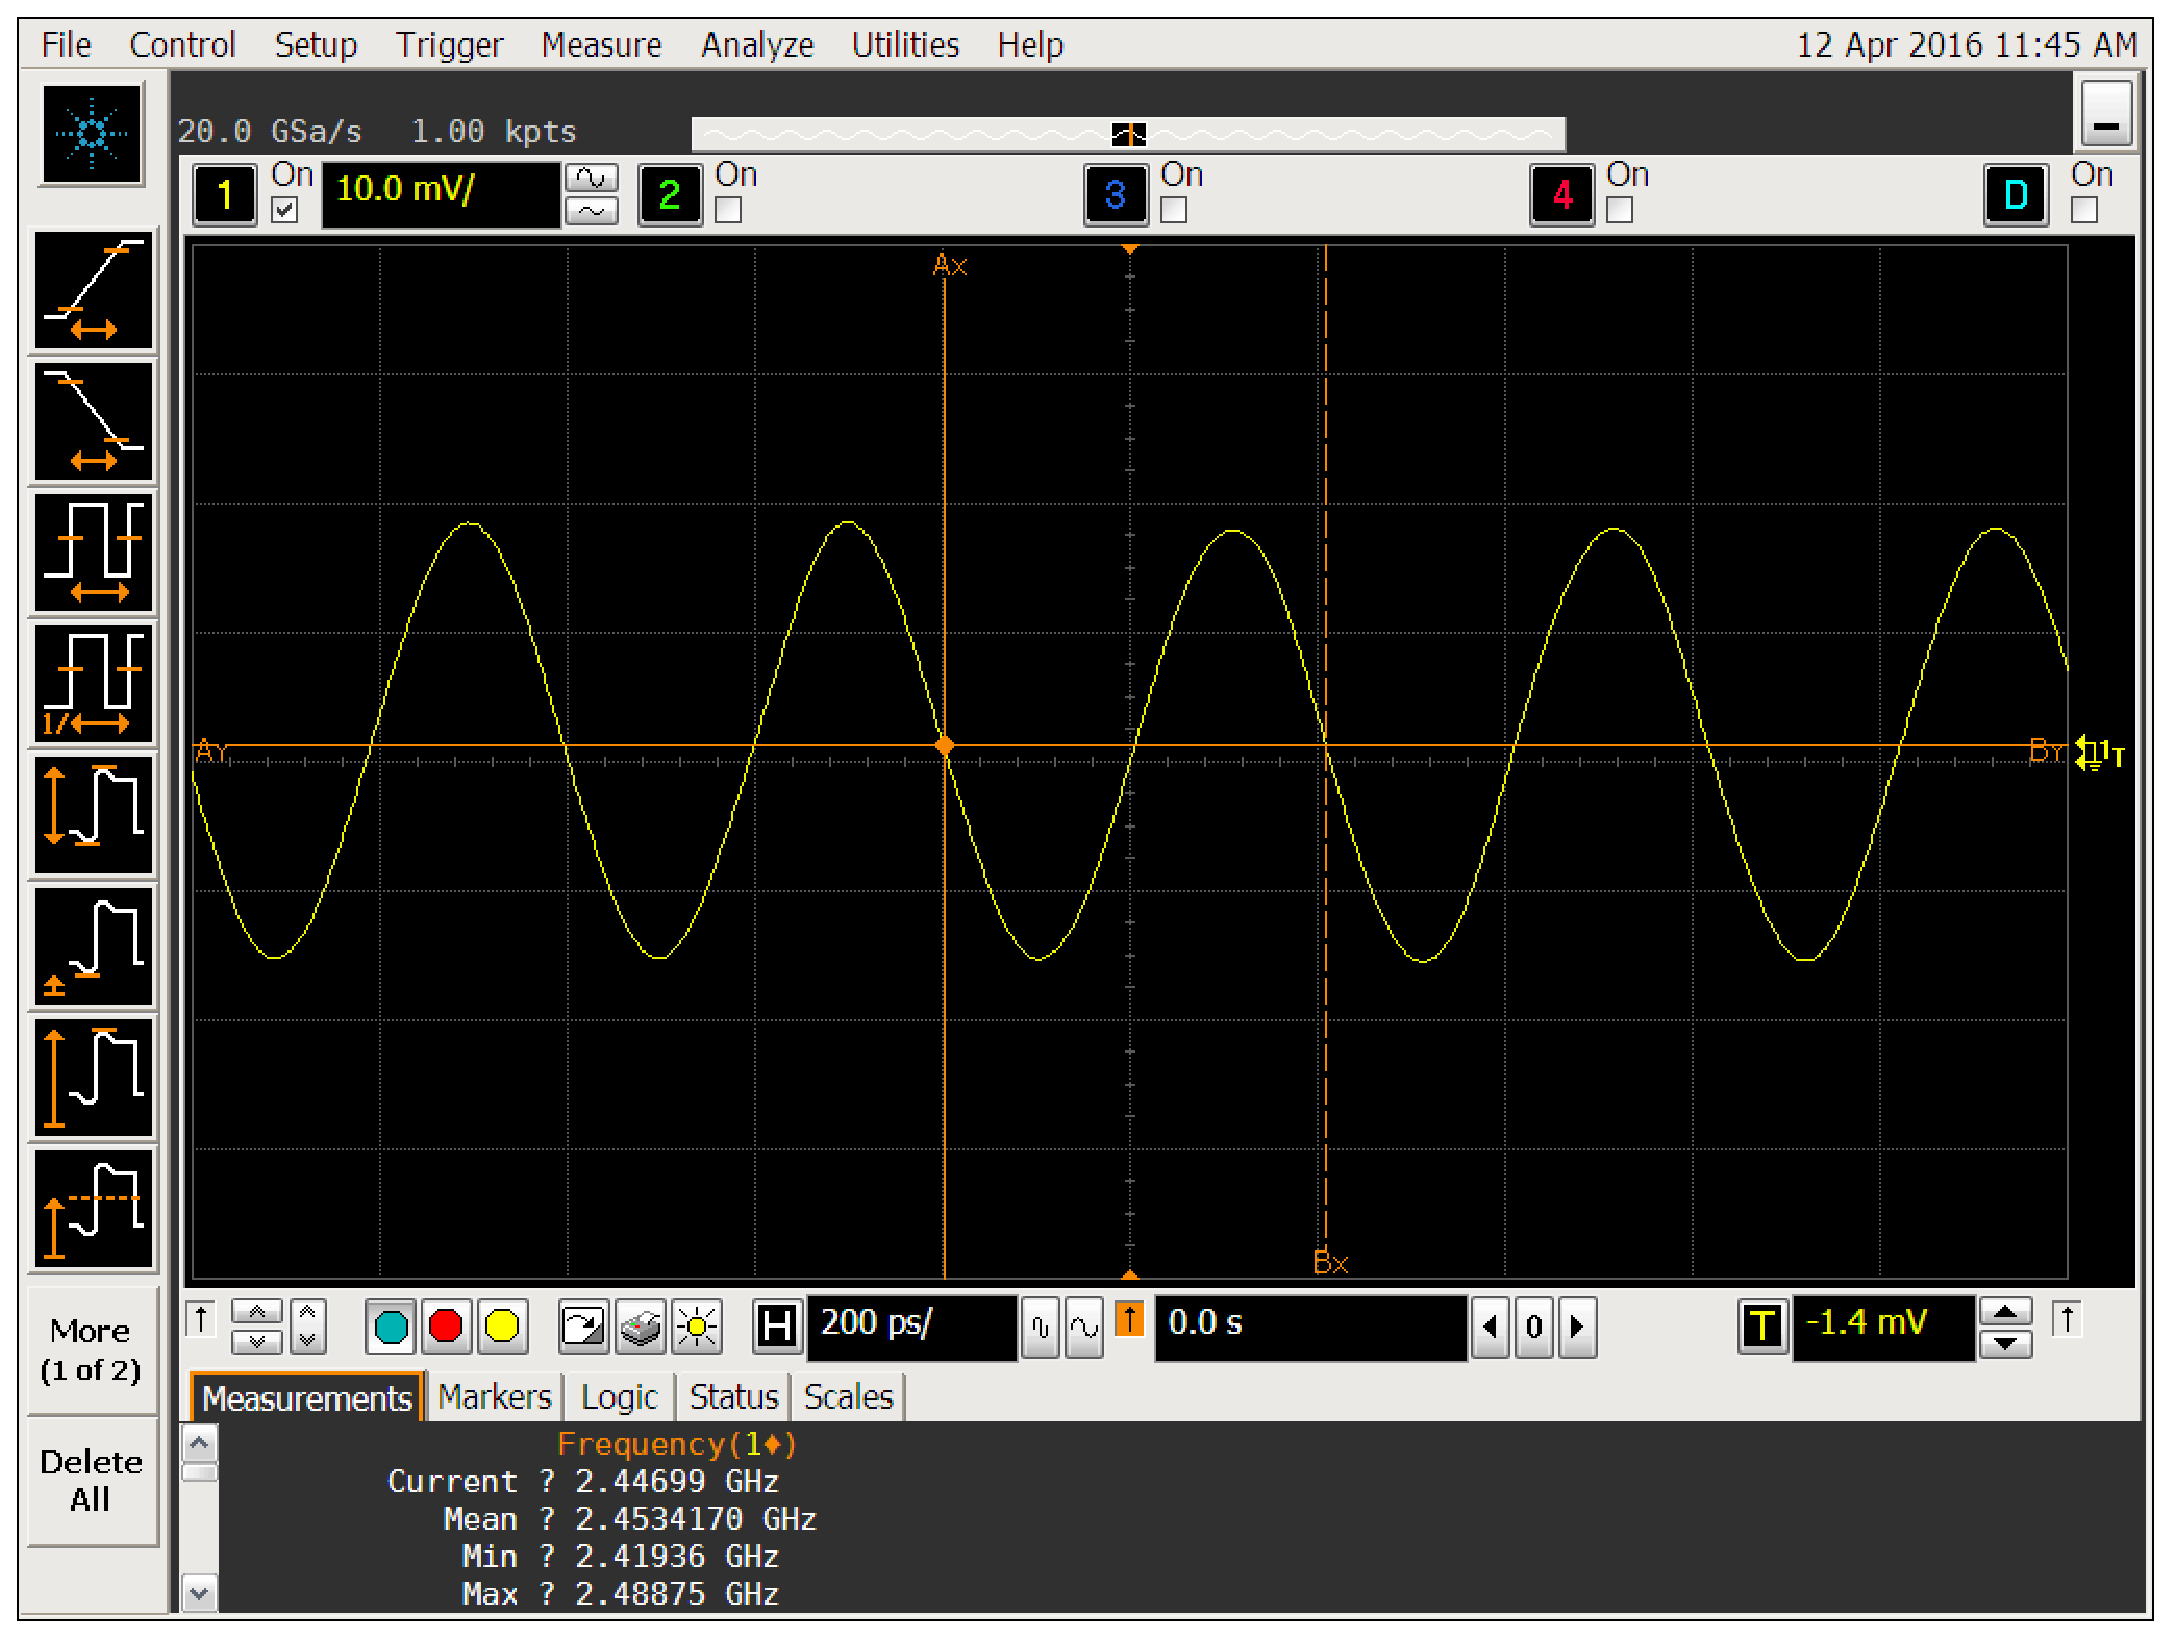
\includegraphics[width=0.85\textwidth]{./figures/oscill_freq}
    \caption{ Carrier Waveform with Frequency Measure
    \label{fig:oscillfreq}}
\end{figure}

%fft config
\begin{figure}[htbp]
    \centering
    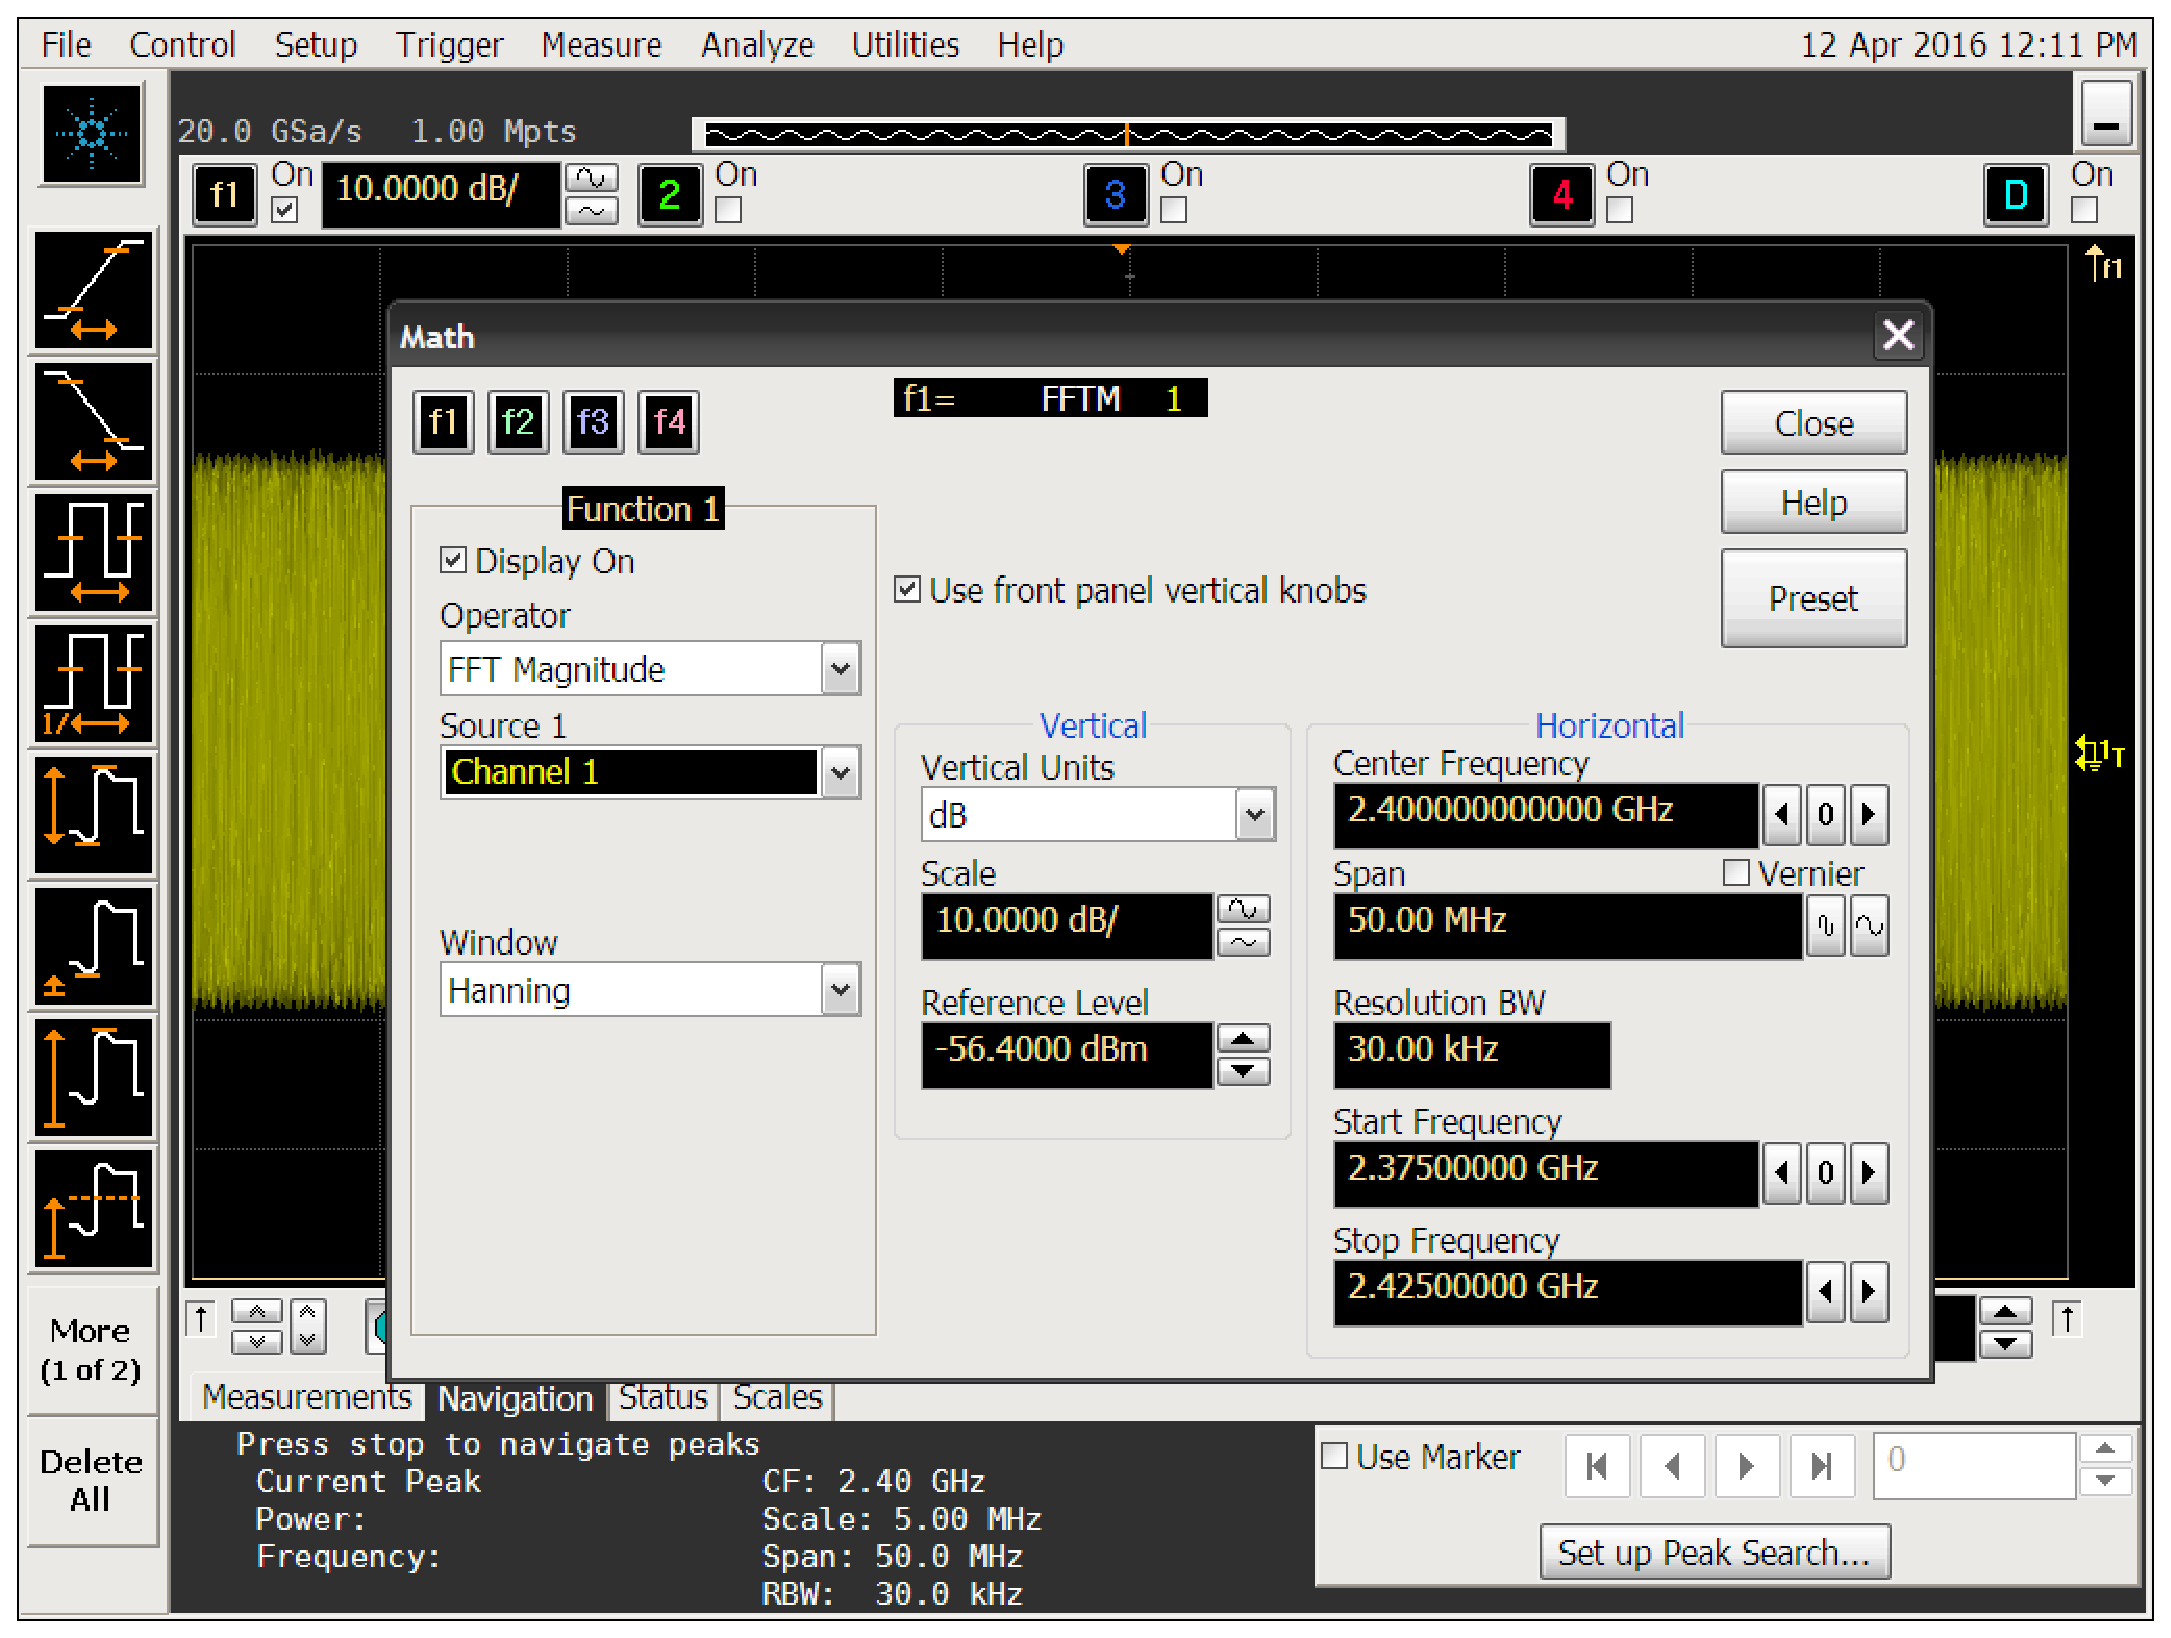
\includegraphics[width=0.85\textwidth]{./figures/oscill_fftcf}
    \caption{ FFT Configuration Parameters
    \label{fig:oscillfftcf}}
\end{figure}

%wave + fft
\begin{figure}[htbp]
    \centering
    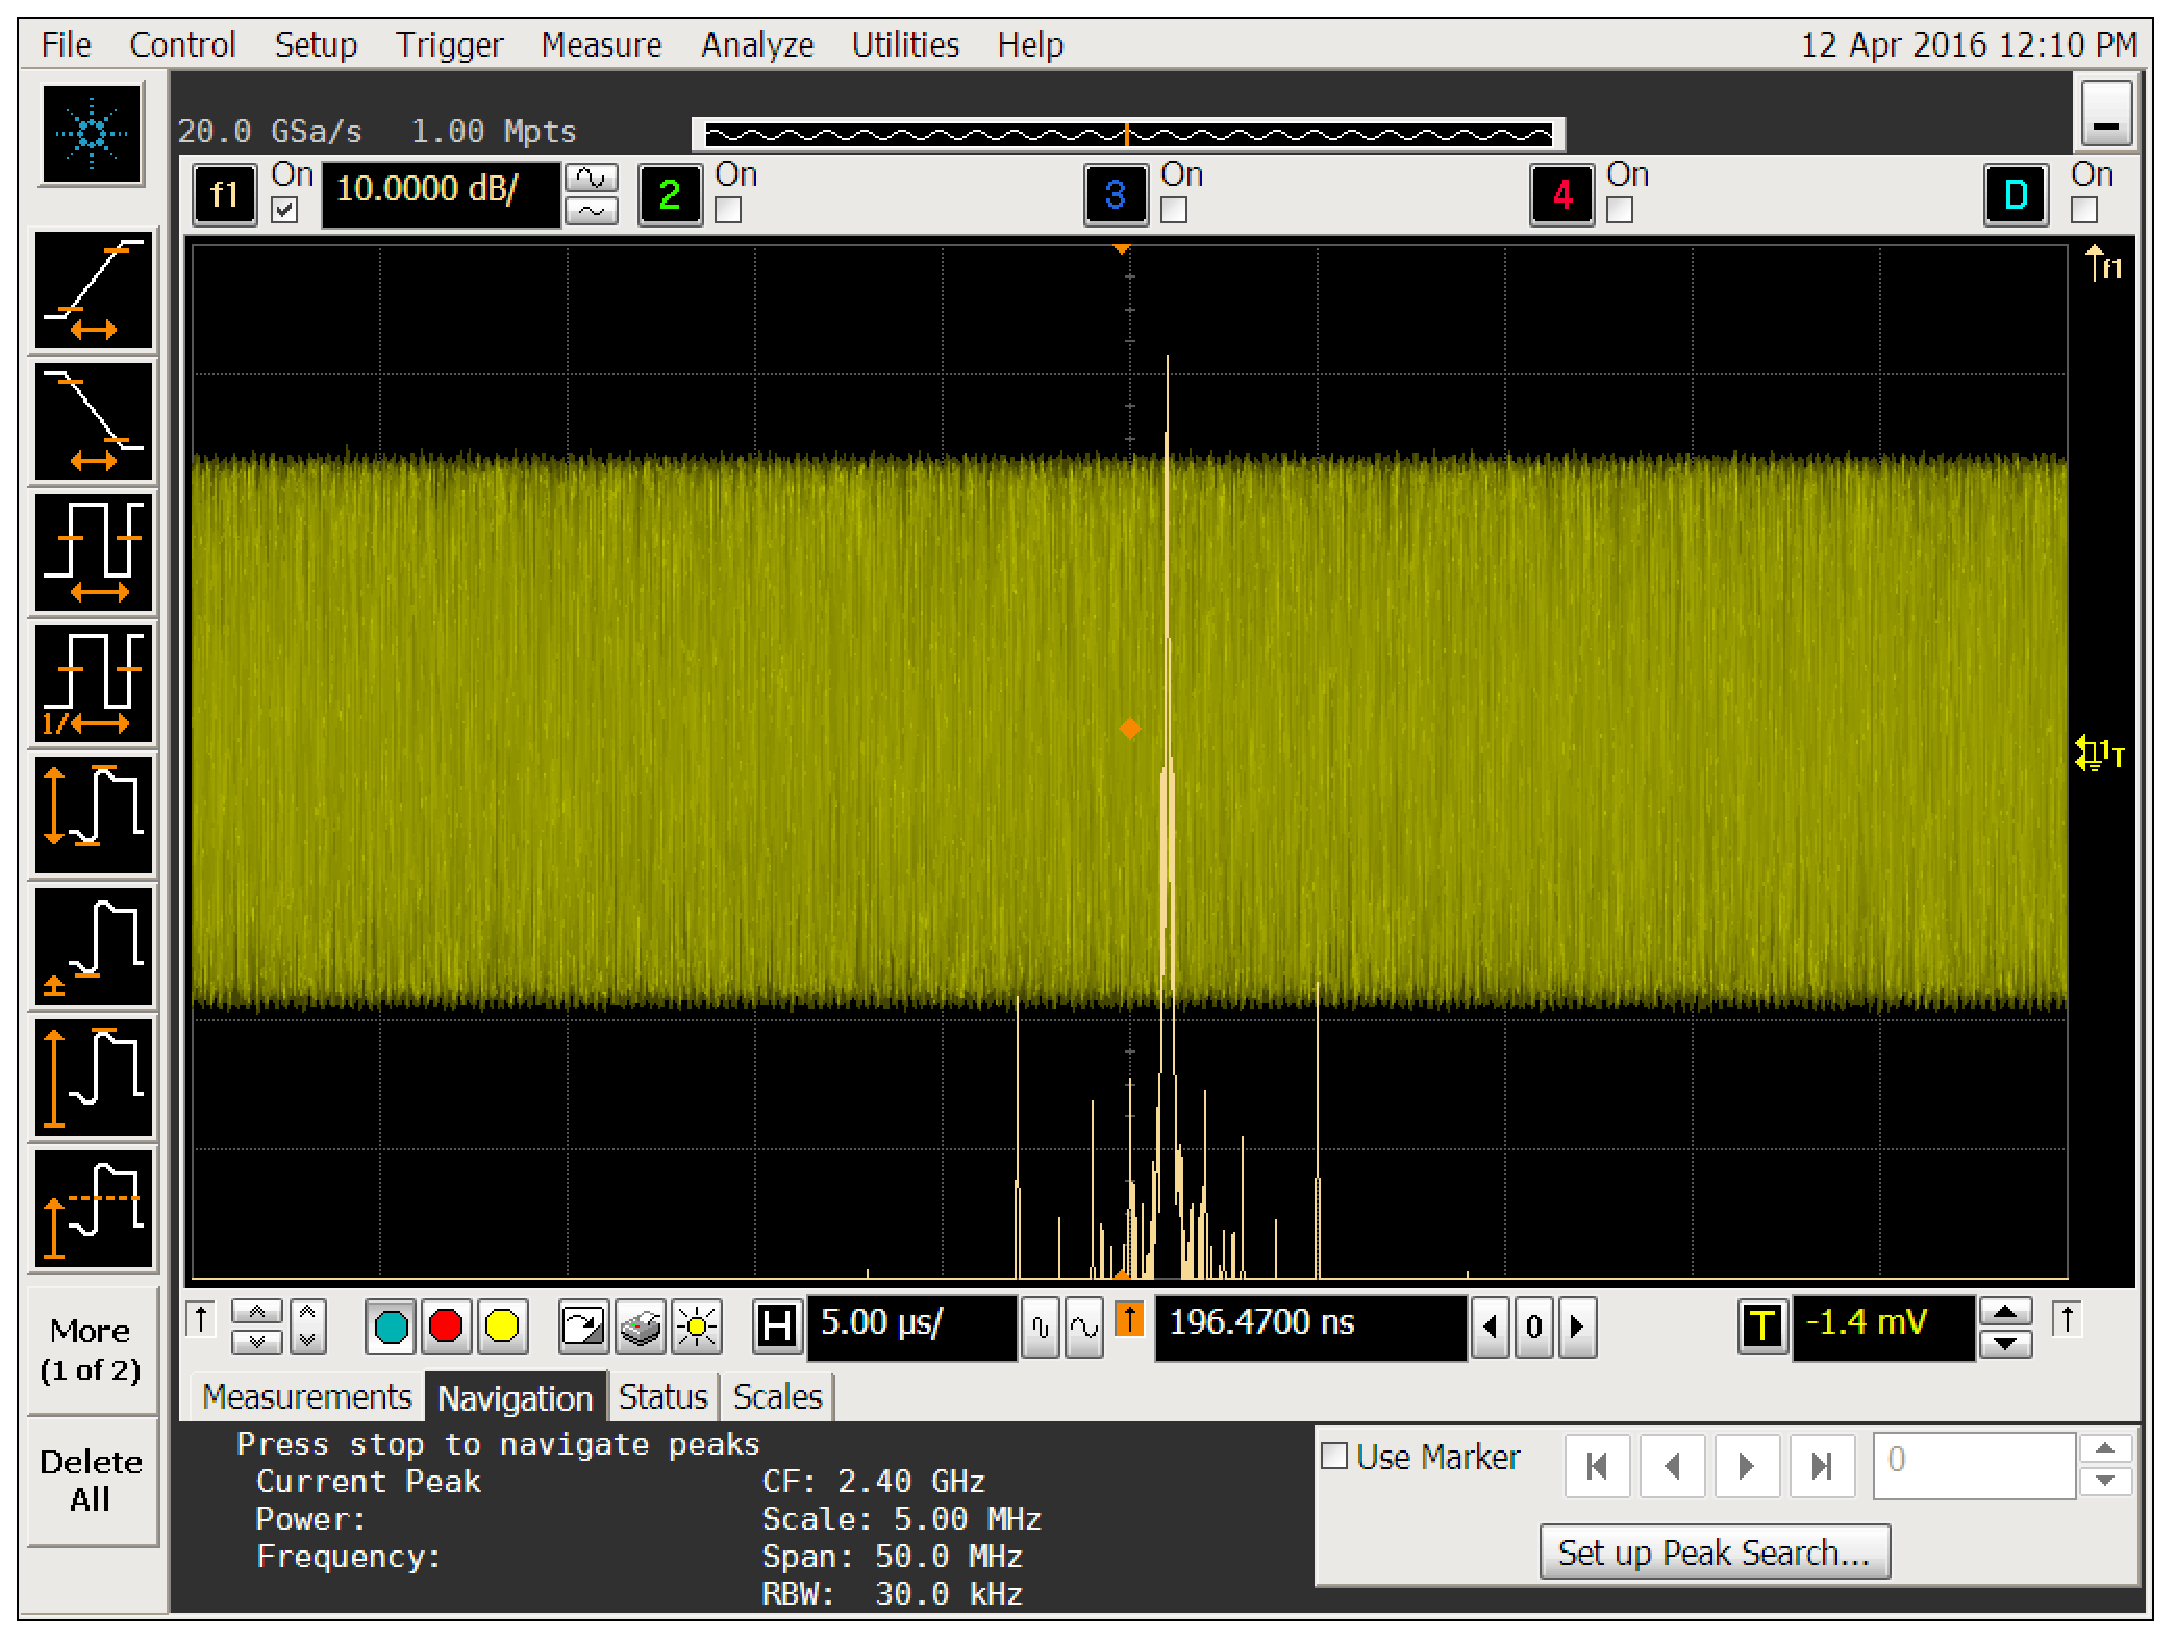
\includegraphics[width=0.85\textwidth]{./figures/oscill_fft}
    \caption{ FFT and Carrier Waveform
    \label{fig:oscillfft}}
\end{figure}

\vfill
\clearpage

\section{Simulation}

An important step in HDL development is the logic simulation of the circuit,
through this simulation it is possible to watch every port and be able to
understand the block behavior, thus correcting any problem or misbehavior.

\subsection{Transmit (DAC) Interface Simulation}

The simulation of the transmit interface, which interfaces the FPGA with DAC was
made in three steps, since the interface is composed by two blocks, there was
the need to simulate each block separately and after this simulate both blocks
connected and working together, in the figures \ref{fig:simdacdma},
\ref{fig:simdac} and \ref{fig:simtxif} it is possible to see the simulation
results and wave diagrams of the three steps.

In the figure \ref{fig:simdacdma} it is possible to watch the behavior of the
\textit{dac-dmaIterface} block where the signal \textit{sig\_dma\_data} is fed to
the block, and the signals \textit{ sig\_axis\_axc0\_itdata, sig\_axis\_axc0\_qtdata,
sig\_axis\_axc1\_itdata and sig\_axis\_axc1\_qtdata} are the \textit{IQ data} being
fed to both to the \textit{dacInterface} block.

\begin{figure}[htbp]
    \centering
    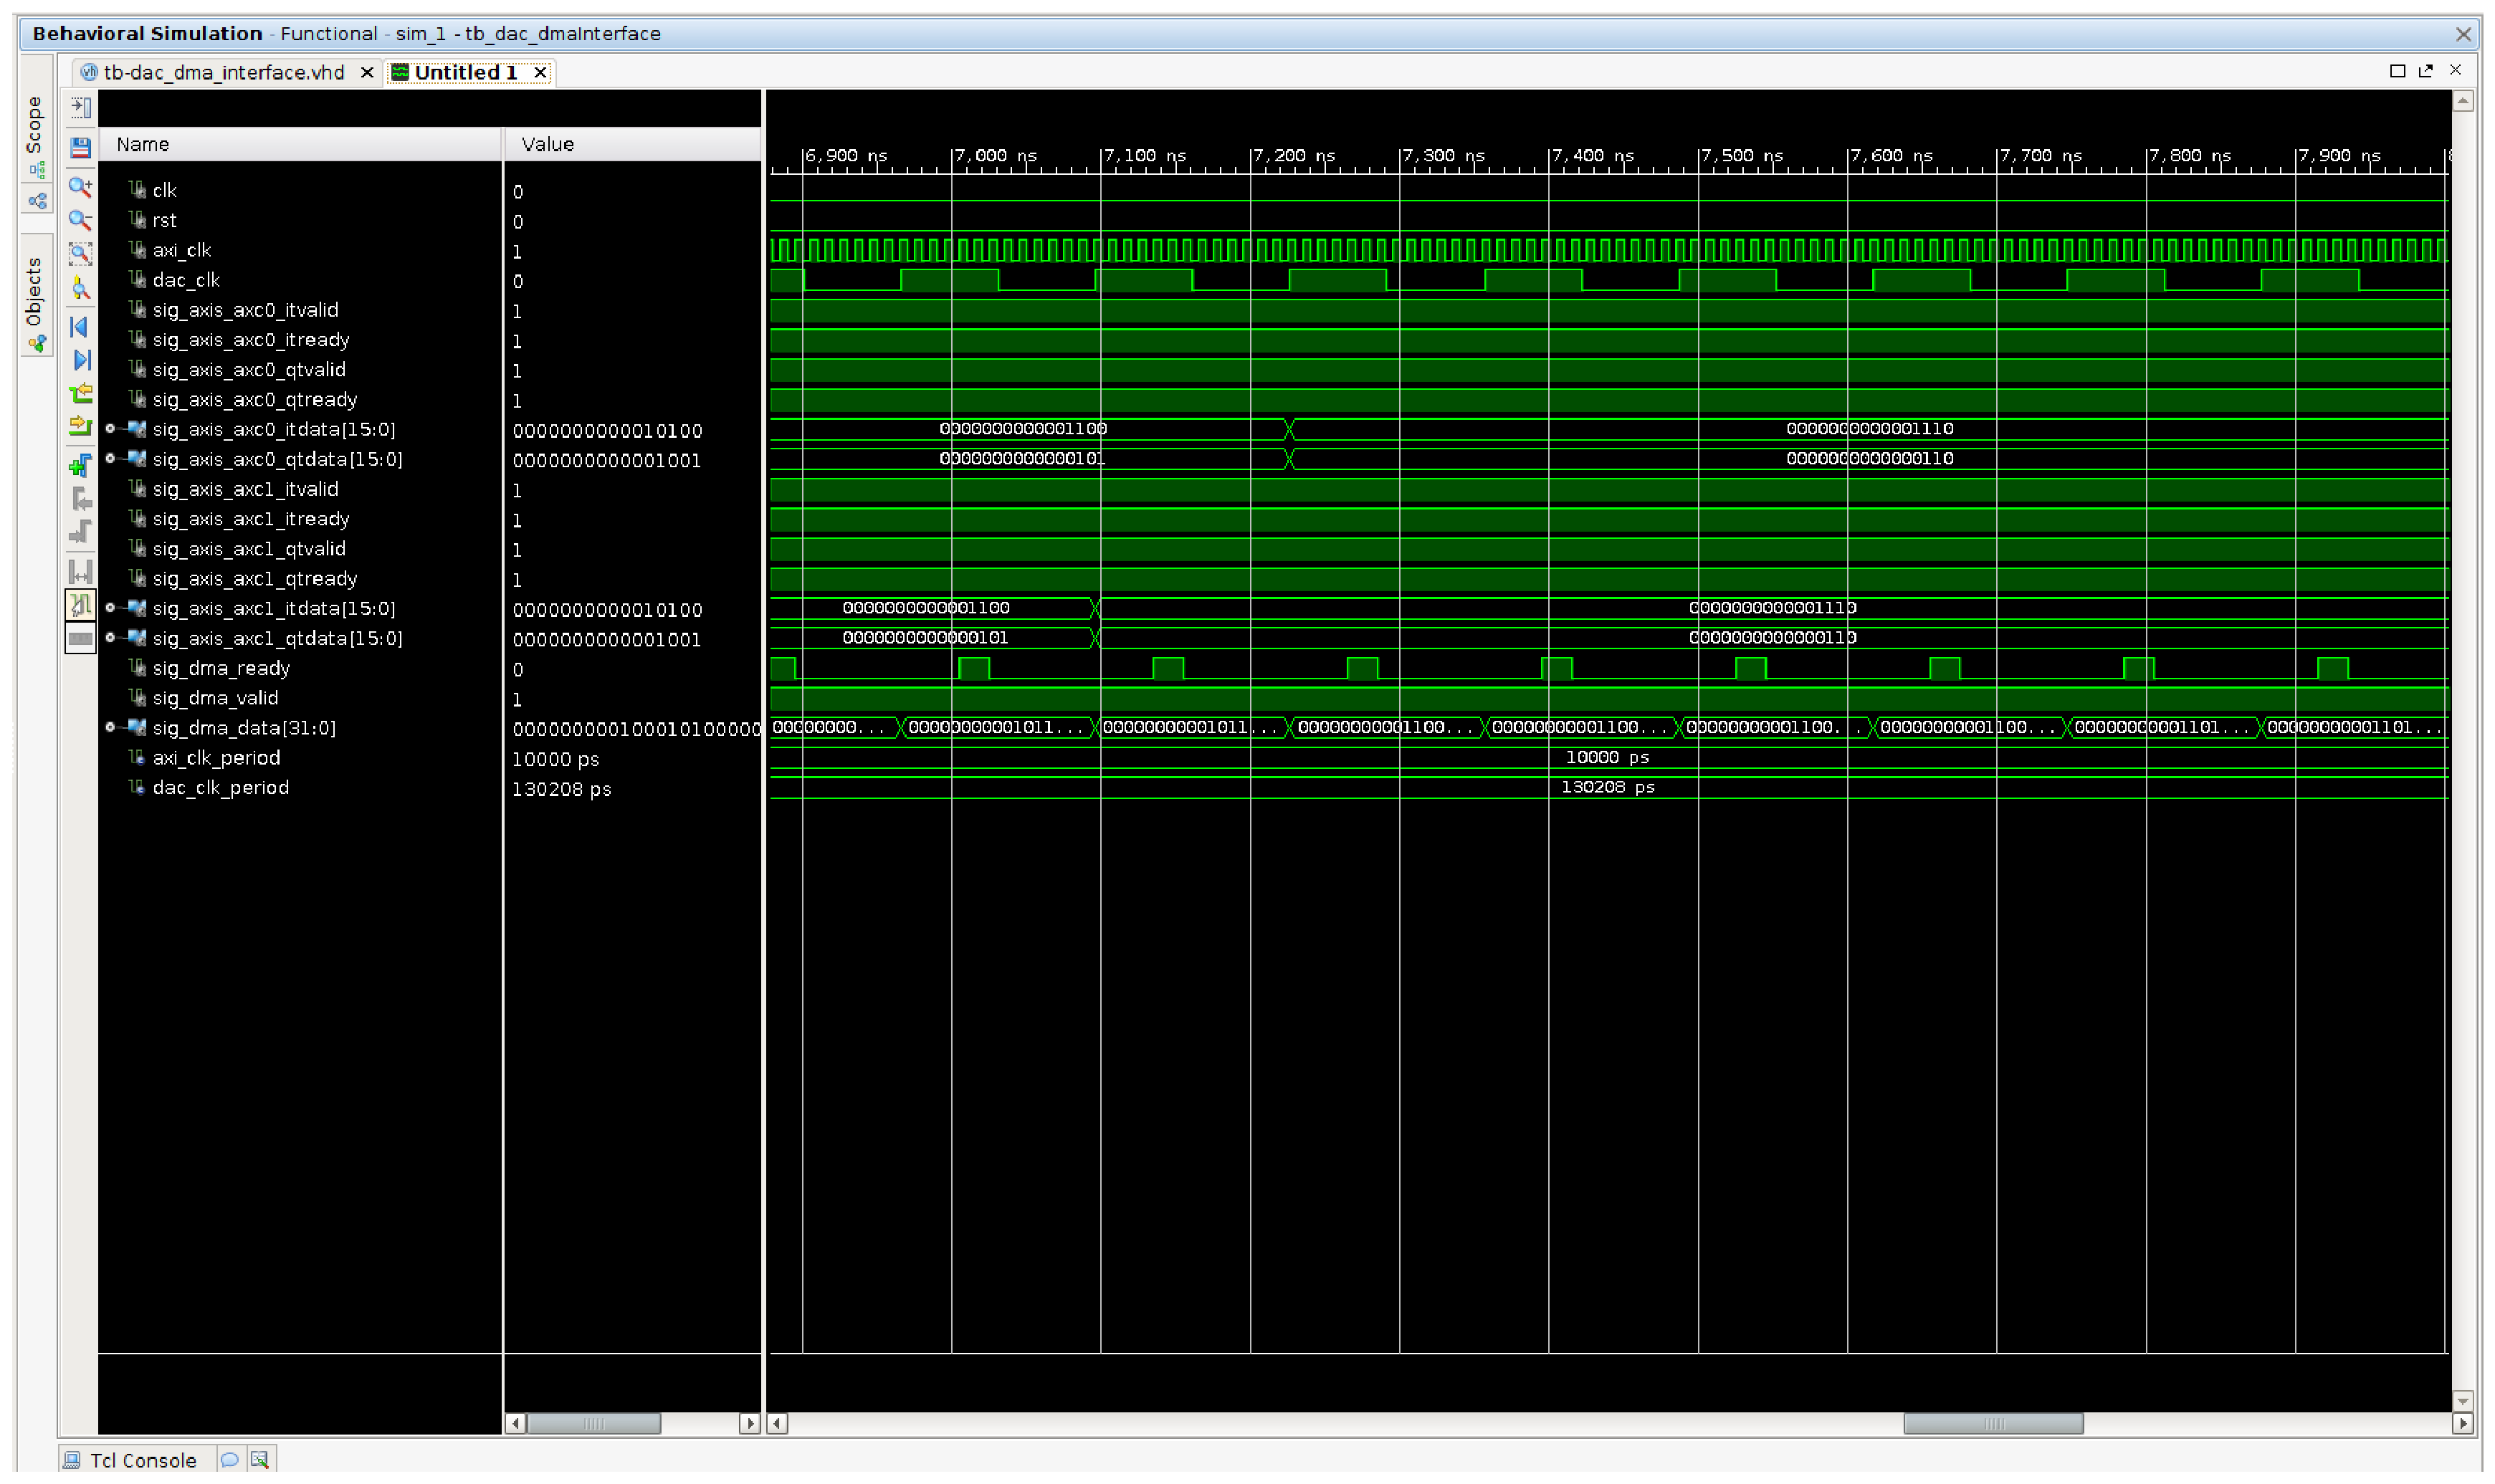
\includegraphics[width=0.95\textwidth]{./figures/dac_dmaInterface}
    \caption{ Step 1: DAC-DMA Interface Block Simulation
    \label{fig:simdacdma}}
\end{figure}

 In the figure \ref{fig:simdac} the \textit{dacInterface} is simulated and again
 it is possible to watch teh signals \textit{sig\_axis\_axc0\_itdata,
 sig\_axis\_axc0\_qtdata, sig\_axis\_axc1\_itdata and sig\_axis\_axc1\_qtdata} being fed
 to the block and the outputs \textit{sig\_dac\_i0data, sig\_dac\_q0data,
 sig\_dac\_i1data and sig\_dac\_q1data}, teh point in both \textit{dac-dmaIterface}
 and \textit{dacInterface} is to watch ghanges in outputs accompanying
 \textit{ready and valid} signals whcih are used as a way of controlling reading
 speed from the \textit{DMA}, in such scheme, the \textit{DMA} assets
 \textit{valid} whenever is can send data, however it only send teh data when
 fed by a ready signal, meaning that the reading block can read the \textit{DMA}
 data.

\begin{figure}[htbp]
    \centering
    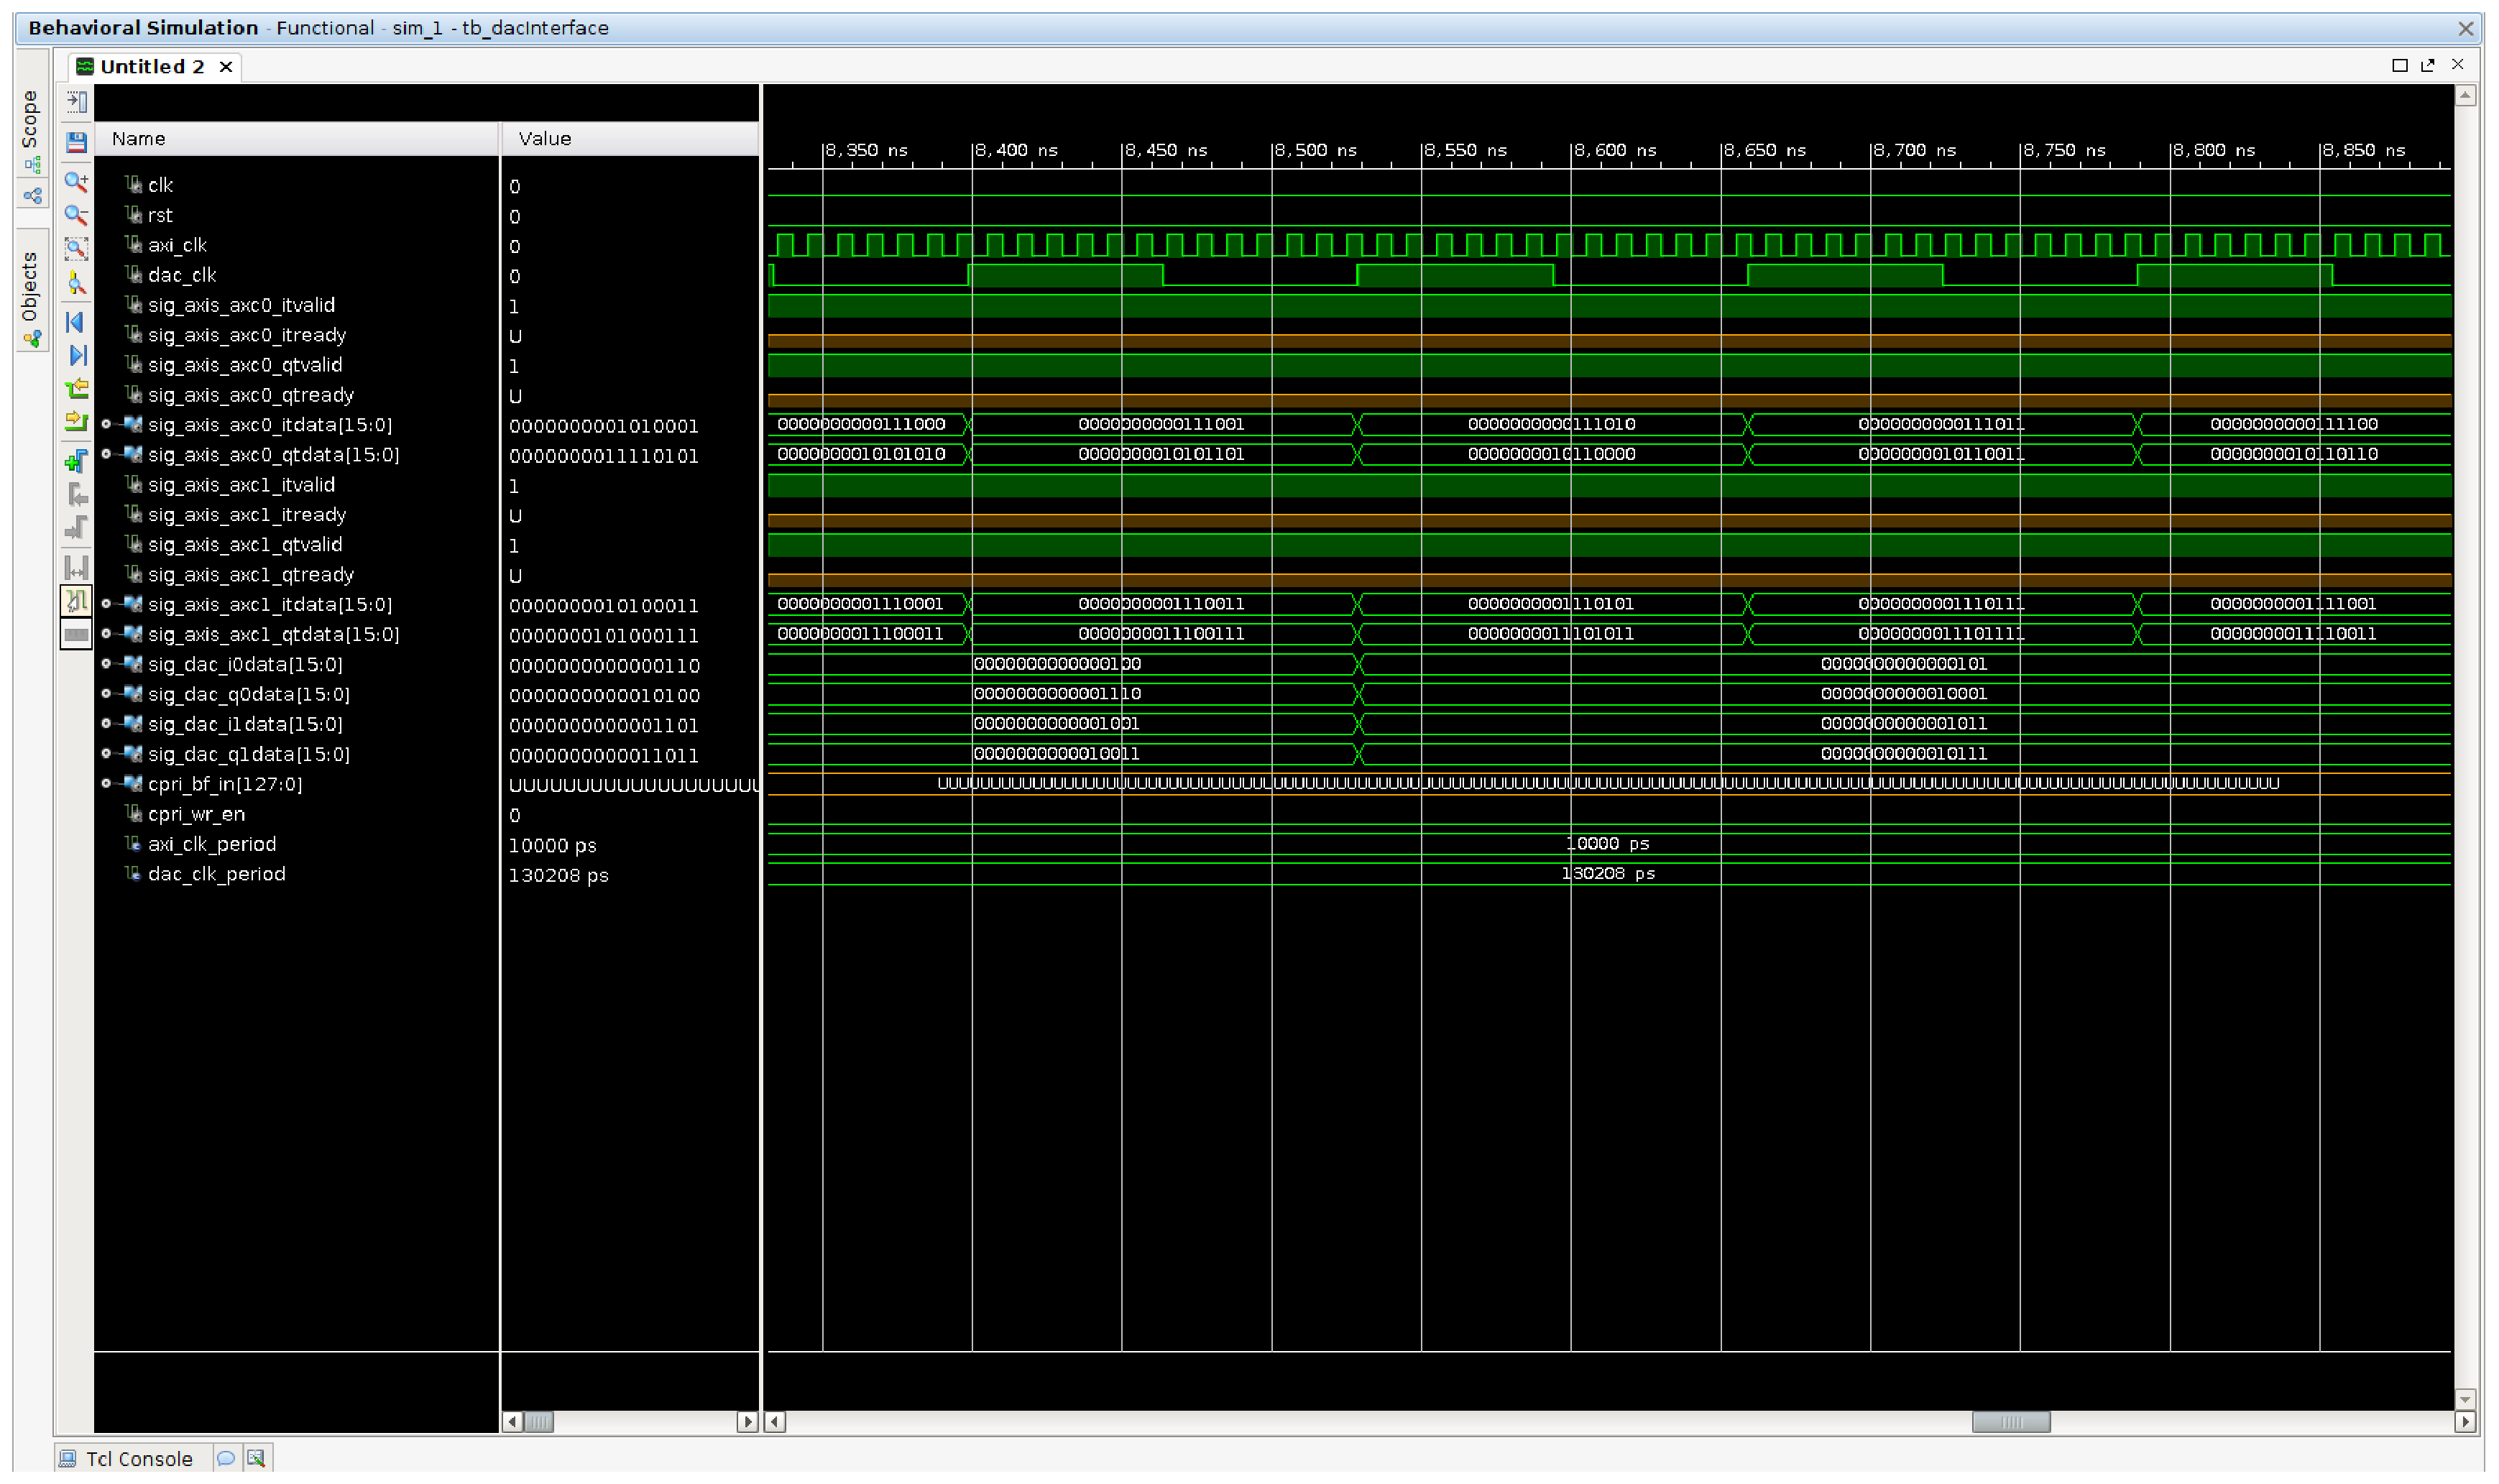
\includegraphics[width=0.95\textwidth]{./figures/dacInterface}
    \caption{ Step 2: DAC Interface Block Simulation
    \label{fig:simdac}}
\end{figure}

In the final simulation of the transmitting interface the whole transmit chain
blocks were simulated toghether and then is is possible to understand the
behavior of the whole transmit interface block. In the figure \ref{fig:simtxif}
it is possible to watch the \textit{DMA} data in the signal in
\textit{dac-dmaIterface} and the outputs which woul fedd the \textit{AD9361}
two \textit{DACs} in the signals \textit{sig\_dac\_i0data, sig\_dac\_q0data,
sig\_dac\_i1data and sig\_dac\_q1data}, again the important thing in the simulation
is to watch for the data change and the  \textit{ready and valid} changes.
Another interesting thing to observ is the two clock variables \textit{axi\_clk}
and \textit{dac\_clk} which represent both axi system clock $ 100 MHz$ and the
dac clock $40 MHz$, this difference justifies the use of such interface.


\begin{figure}[htbp]
    \centering
    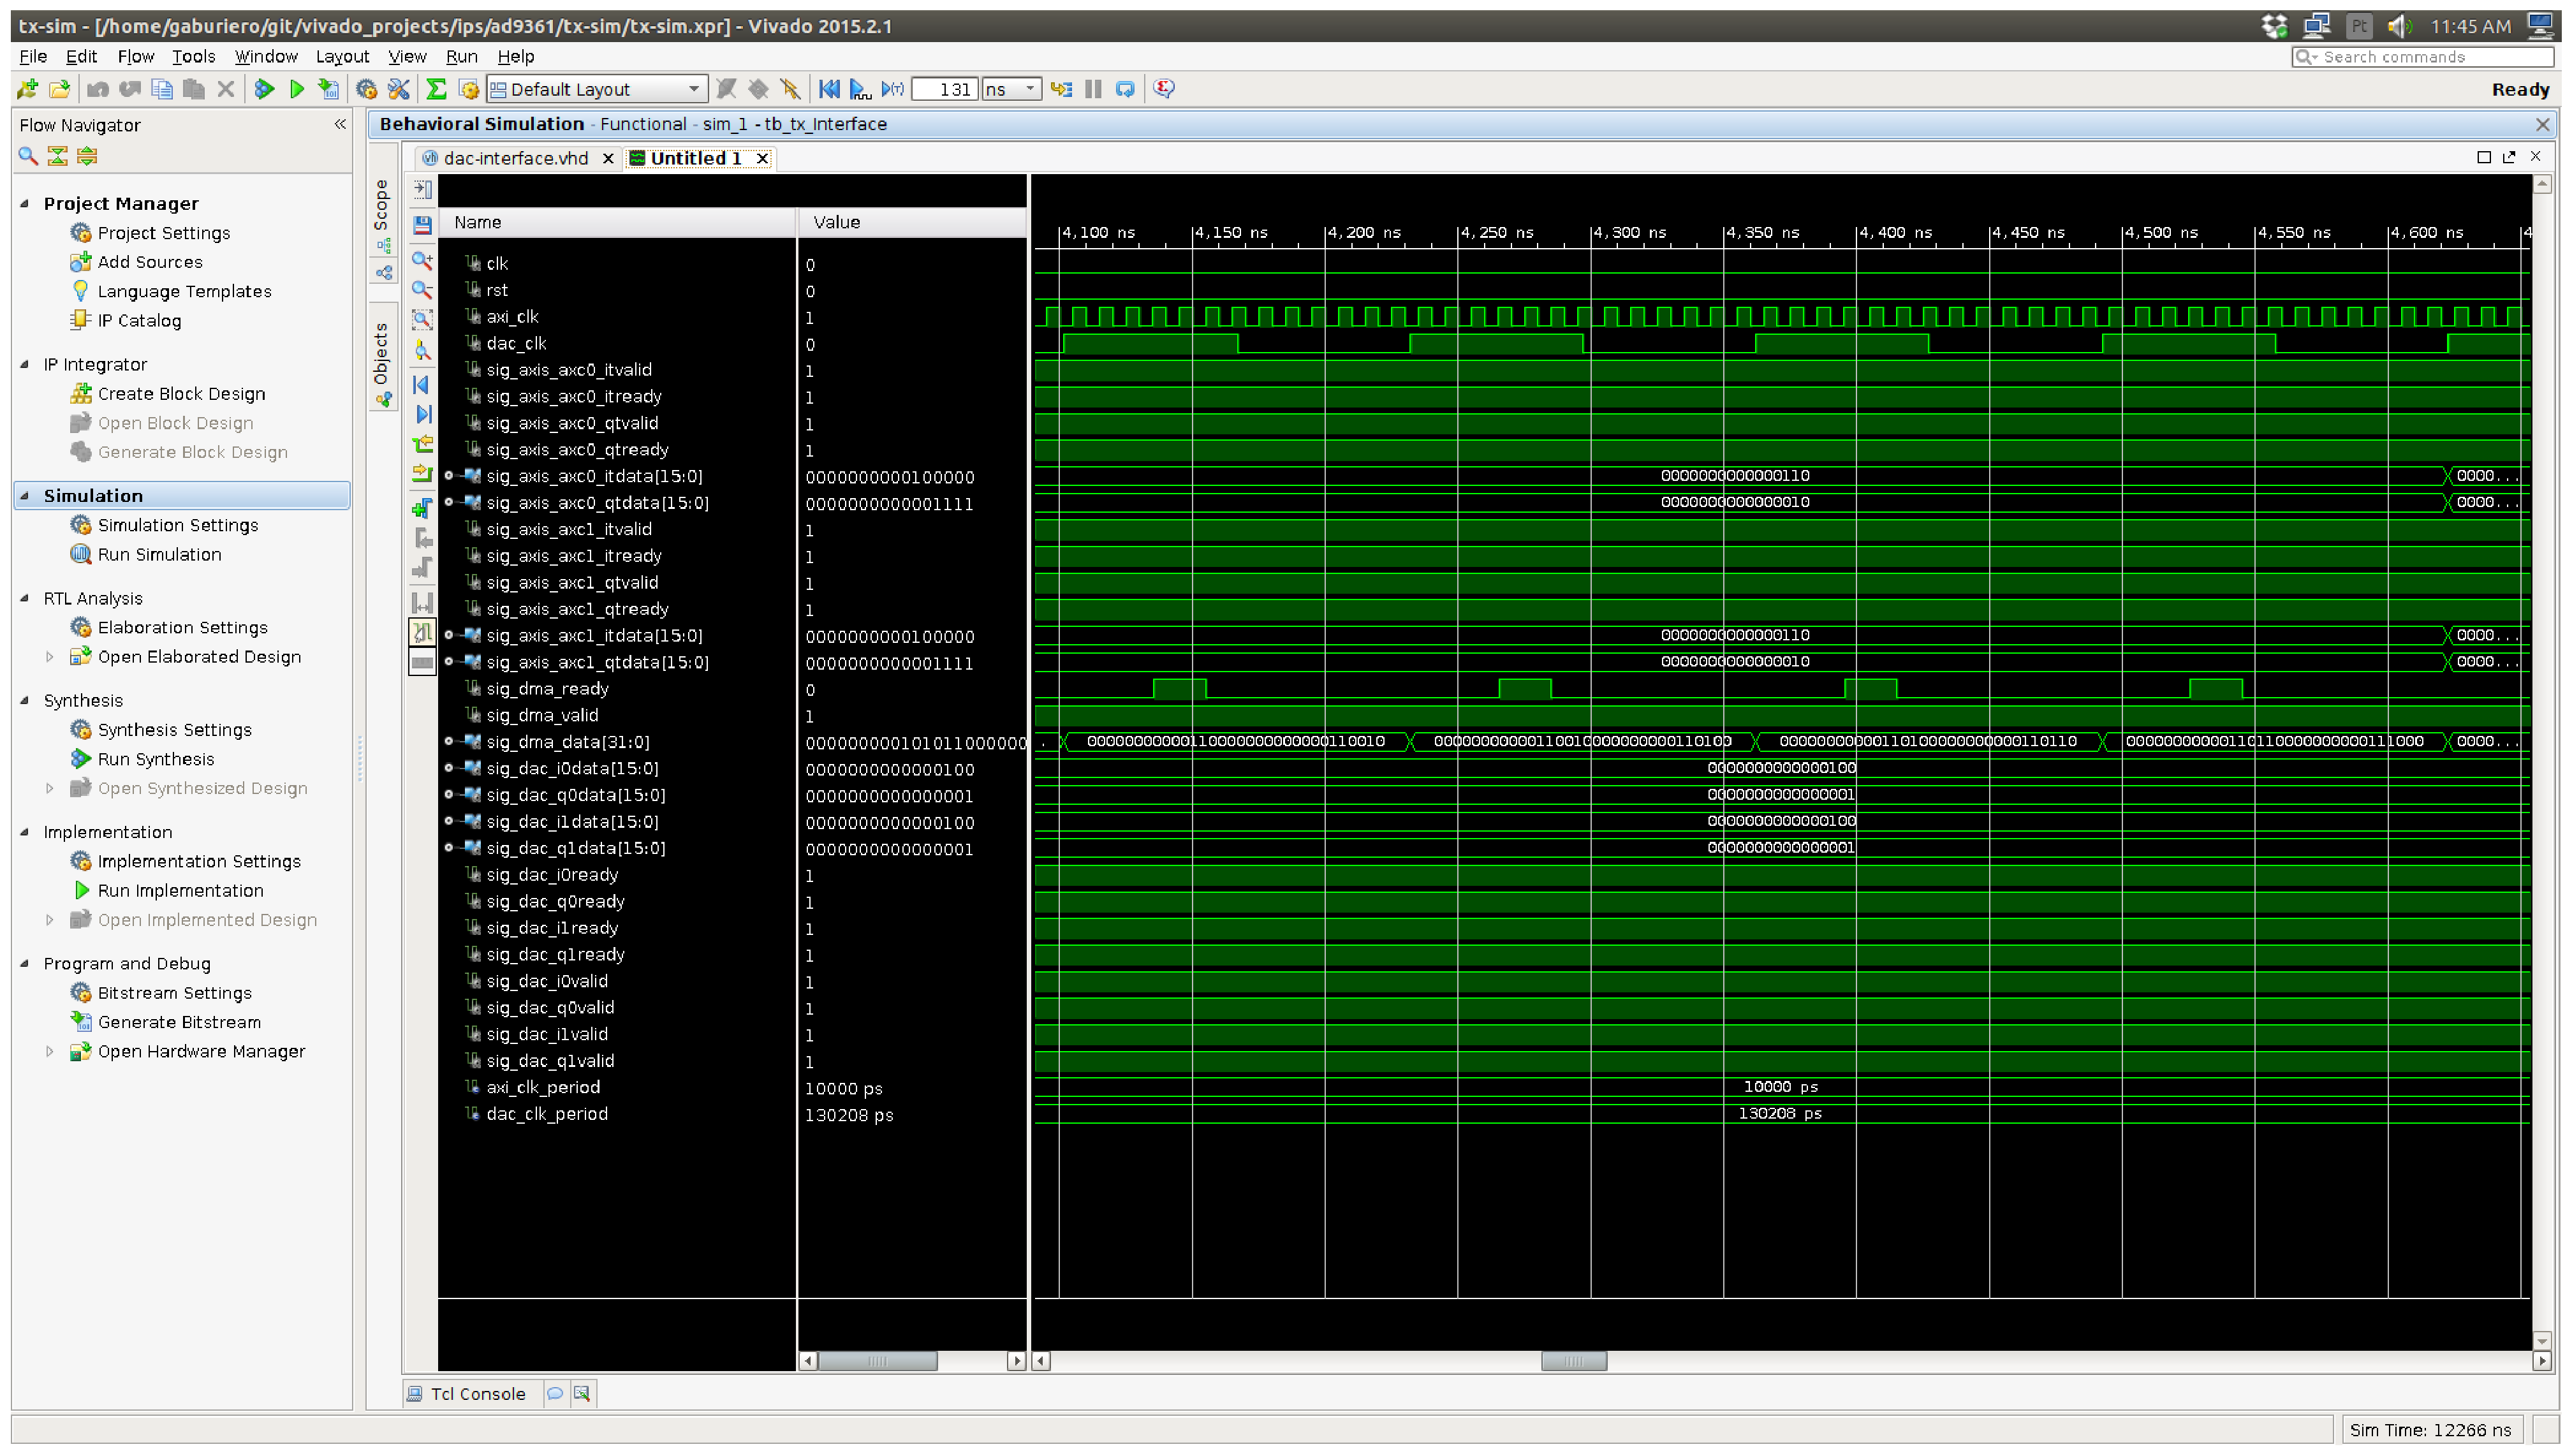
\includegraphics[width=0.95\textwidth]{./figures/txInterface}
    \caption{ Step 3: Transmitting Interface Block Simulation
    \label{fig:simtxif}}
\end{figure}

\subsection{Receive (ADC) Interface Simulation}

As stated before on chapter \ref{chap:implementation} in the section \ref{impl:setup},
the DAC interface is simple beacause the data input is already limited by the DAC
clock, so there is no need to make a bottleneck like in the DAC interface.

 In the figure \ref{fig:simdac} it is possible to see the output and wave
diagram in the simulation window. Since the \textit{adcInterface} is much more
simpler, because the data input is already limited by the \textit{AD9361}
clock, in the signals \textit{sig\_rx\_i0\_data, sig\_rx\_q0\_data,
sig\_rx\_i1\_data, sig\_rx\_q1\_data} there is the outputs from both
\textit{DACs} and \textit{dout} is the data that will be fed to the
\textit{DMA}.\\

\begin{figure}[htbp]
    \centering
    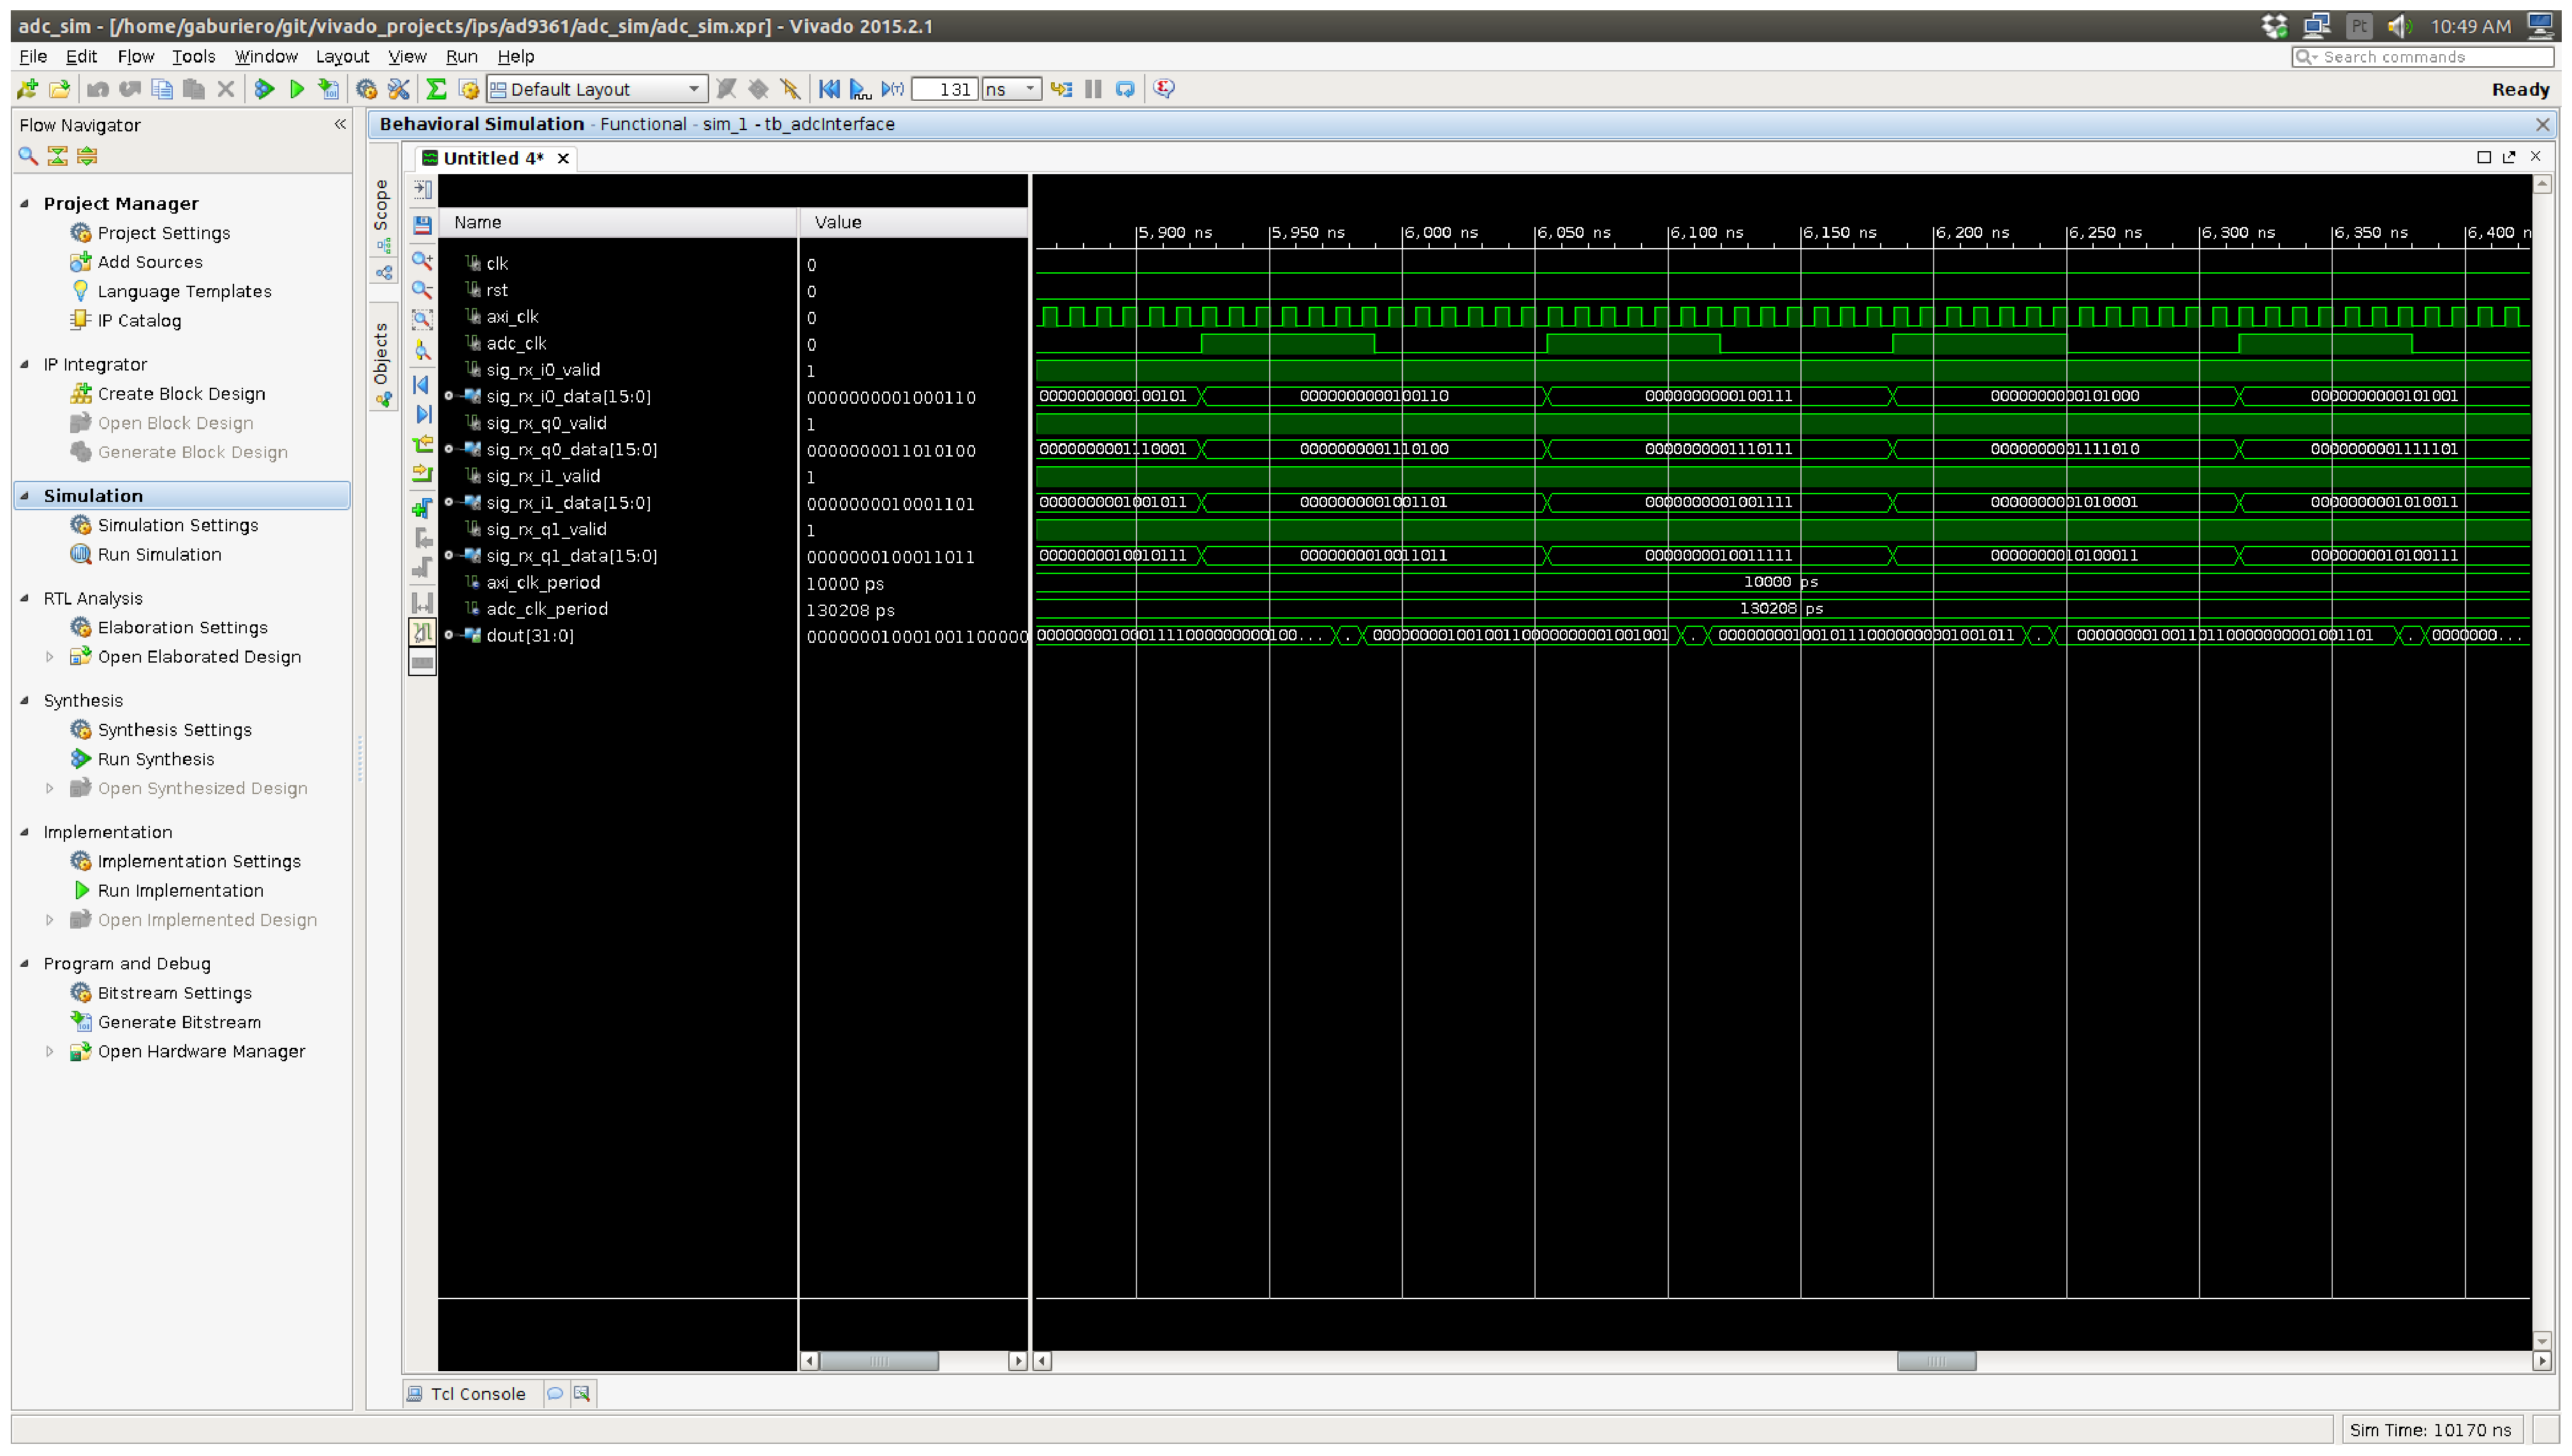
\includegraphics[width=0.95\textwidth]{./figures/adcInterface}
    \caption{ ADC Interface Block Simulation
    \label{fig:simadc}}
\end{figure}

\vfill
\clearpage

\section{Transmission Tests (DAC)}
\label{result:dac}

 The transmission tests aim to evaluate a Donwlink LTE transmission, it means
that the data is being transmitted from the BTS to the UE. In this trnasmission
test there were generated LTE samples in matlab, and these samples were loaded
in the memory by putting them in a header file, the as explained before, DMA
shall read them and the DAC shall make an analog output. In the figure
\ref{fig:dacsignals} there are the DAC control signals sent to the data
interface block in order to control the data flow, thus this control makes a
back-pressure in the DMA engine controlling if DMA reads or not data from
memory, thus the DMA Engine reading output can be seen in the figures
\ref{fig:dataflowdig} and \ref{fig:dataflowana}, digital and analog waveforms
respectively.\\

 It is possible to configure in the driver if the AD9361 ouputs or not a clock
in a special clock\_output pin, so in order to evaluate frequency and clock
quality, the figure \ref{fig:dacclk} shows the clock output from the AD9361 and
last but not least the figure \ref{fig:lte5m} show the output spectrum of the
LTE analog wave outputted from the FMComms2 board.

\begin{figure}[htbp]
    \centering
    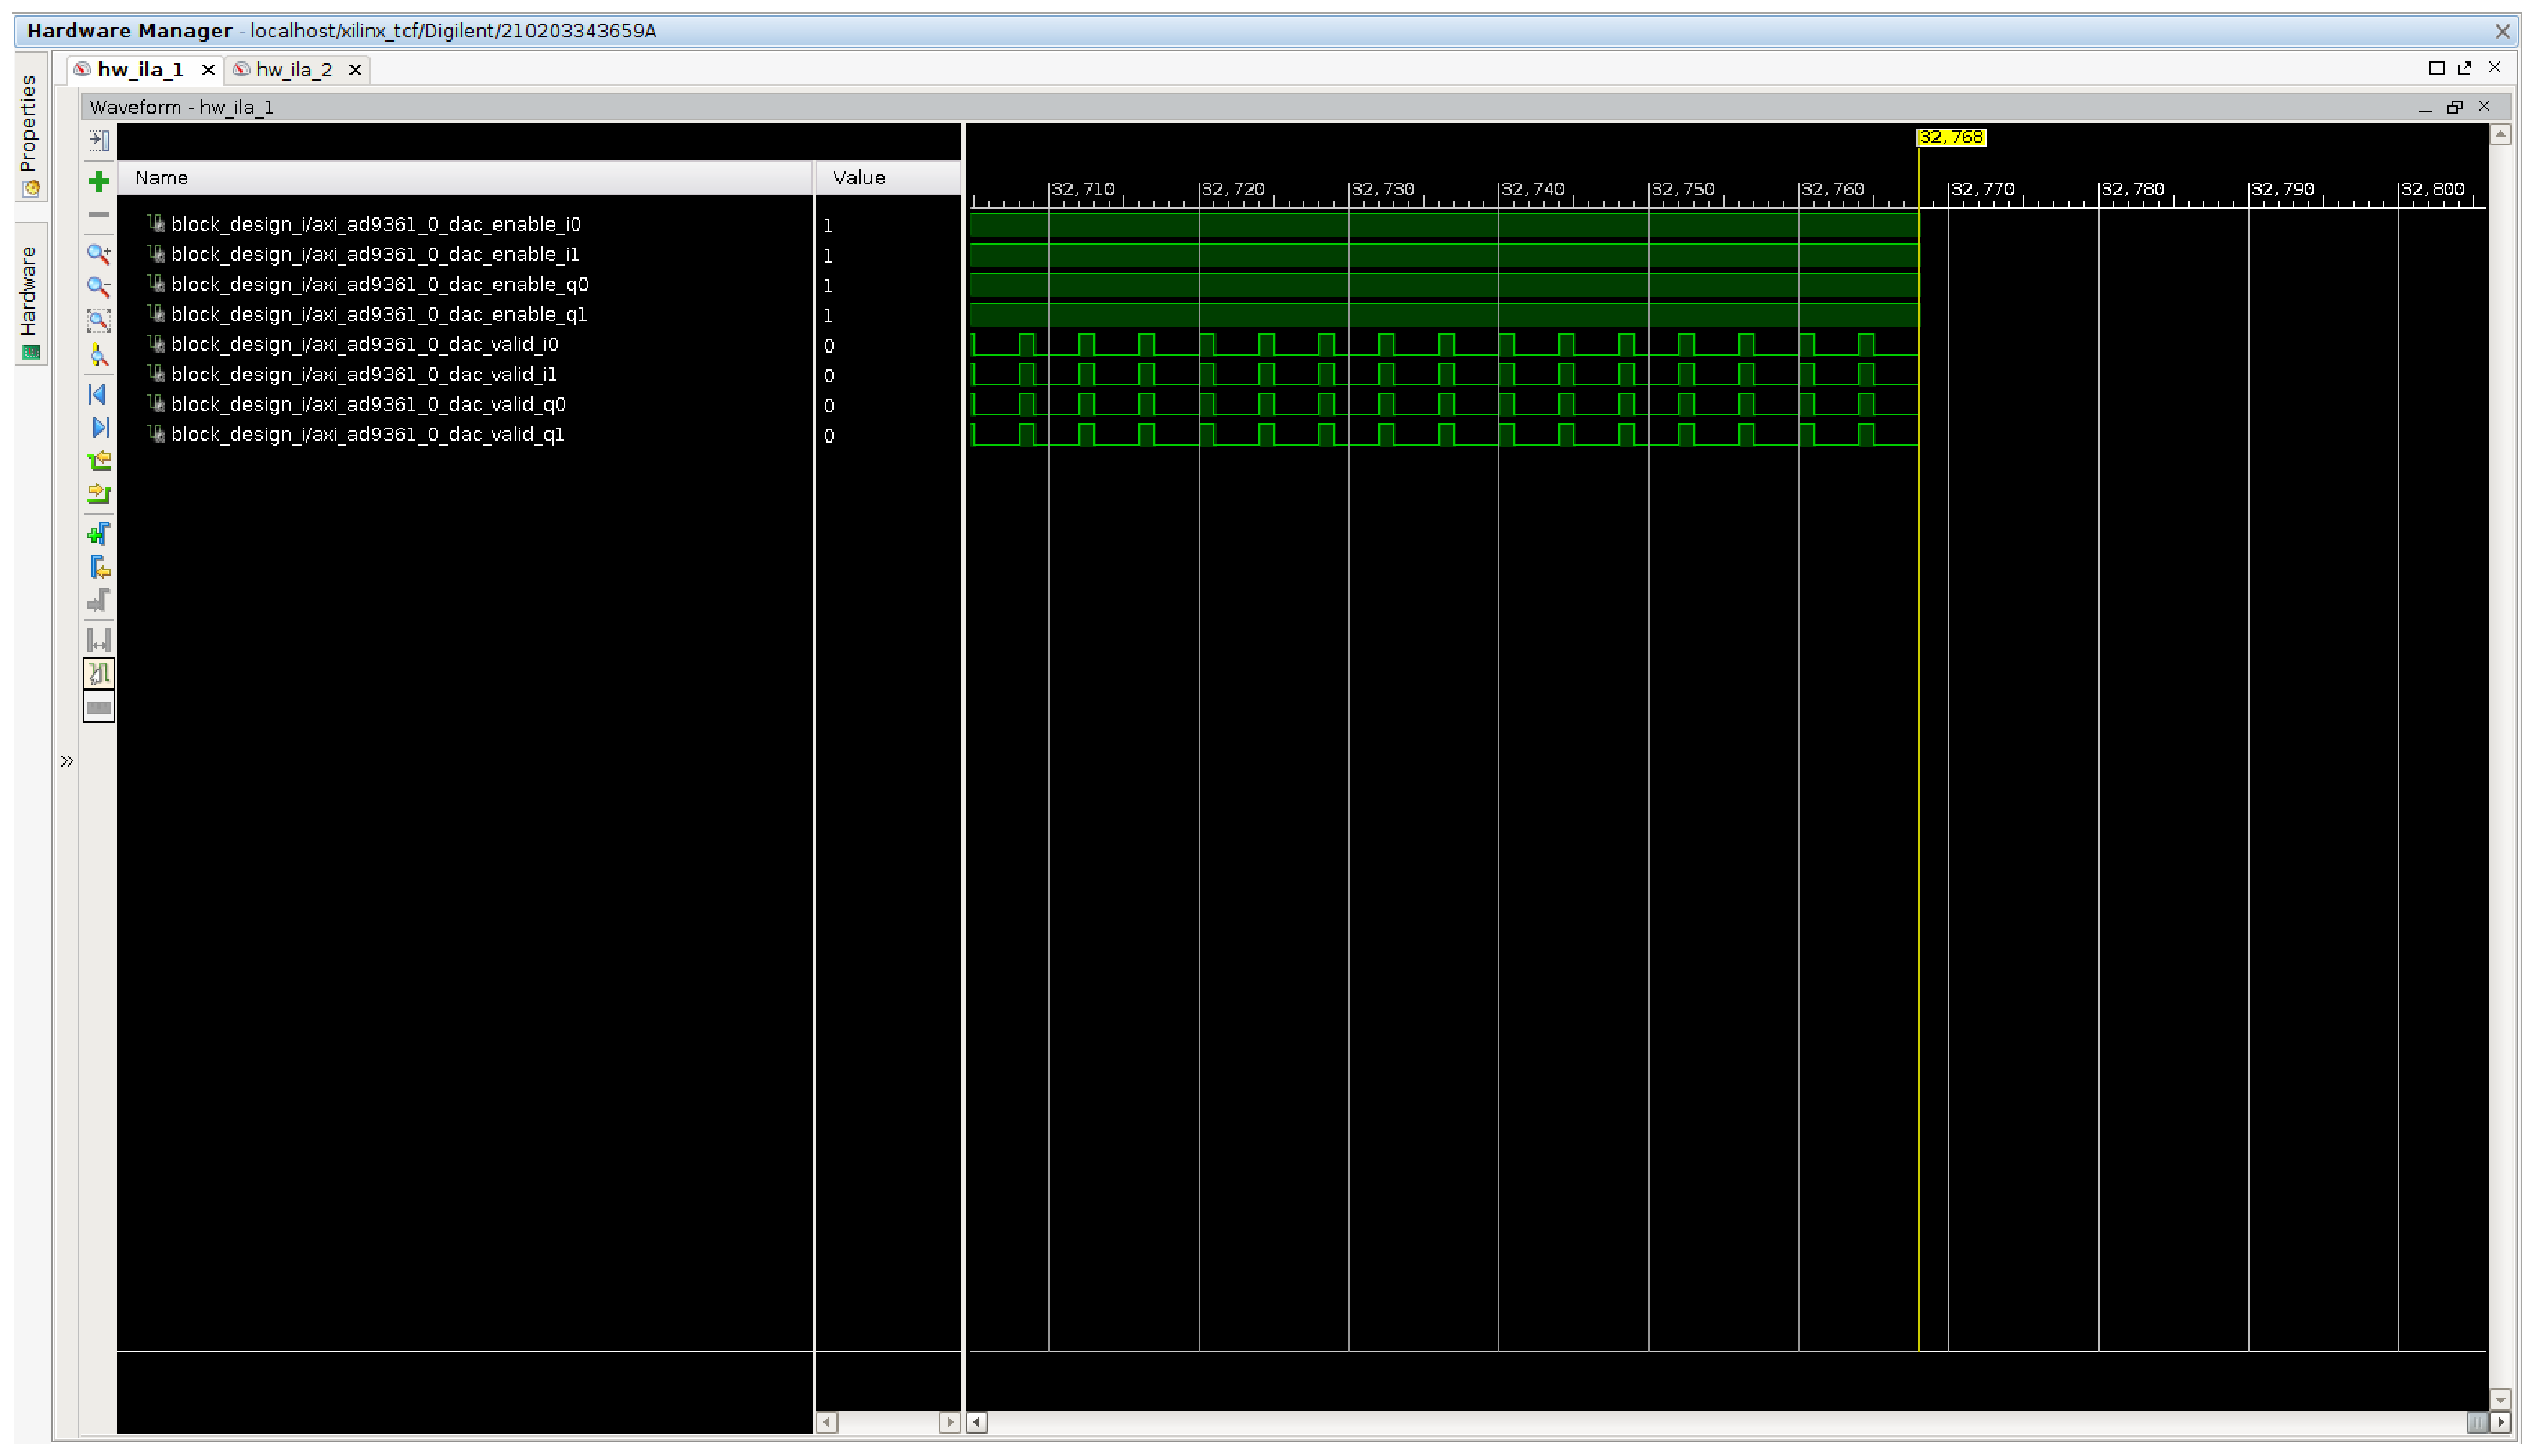
\includegraphics[width=0.85\textwidth]{./figures/dac_signals}
    \caption{ DAC signals controlling data reading
    \label{fig:dacsignals}}
\end{figure}

\begin{figure}[htbp]
    \centering
    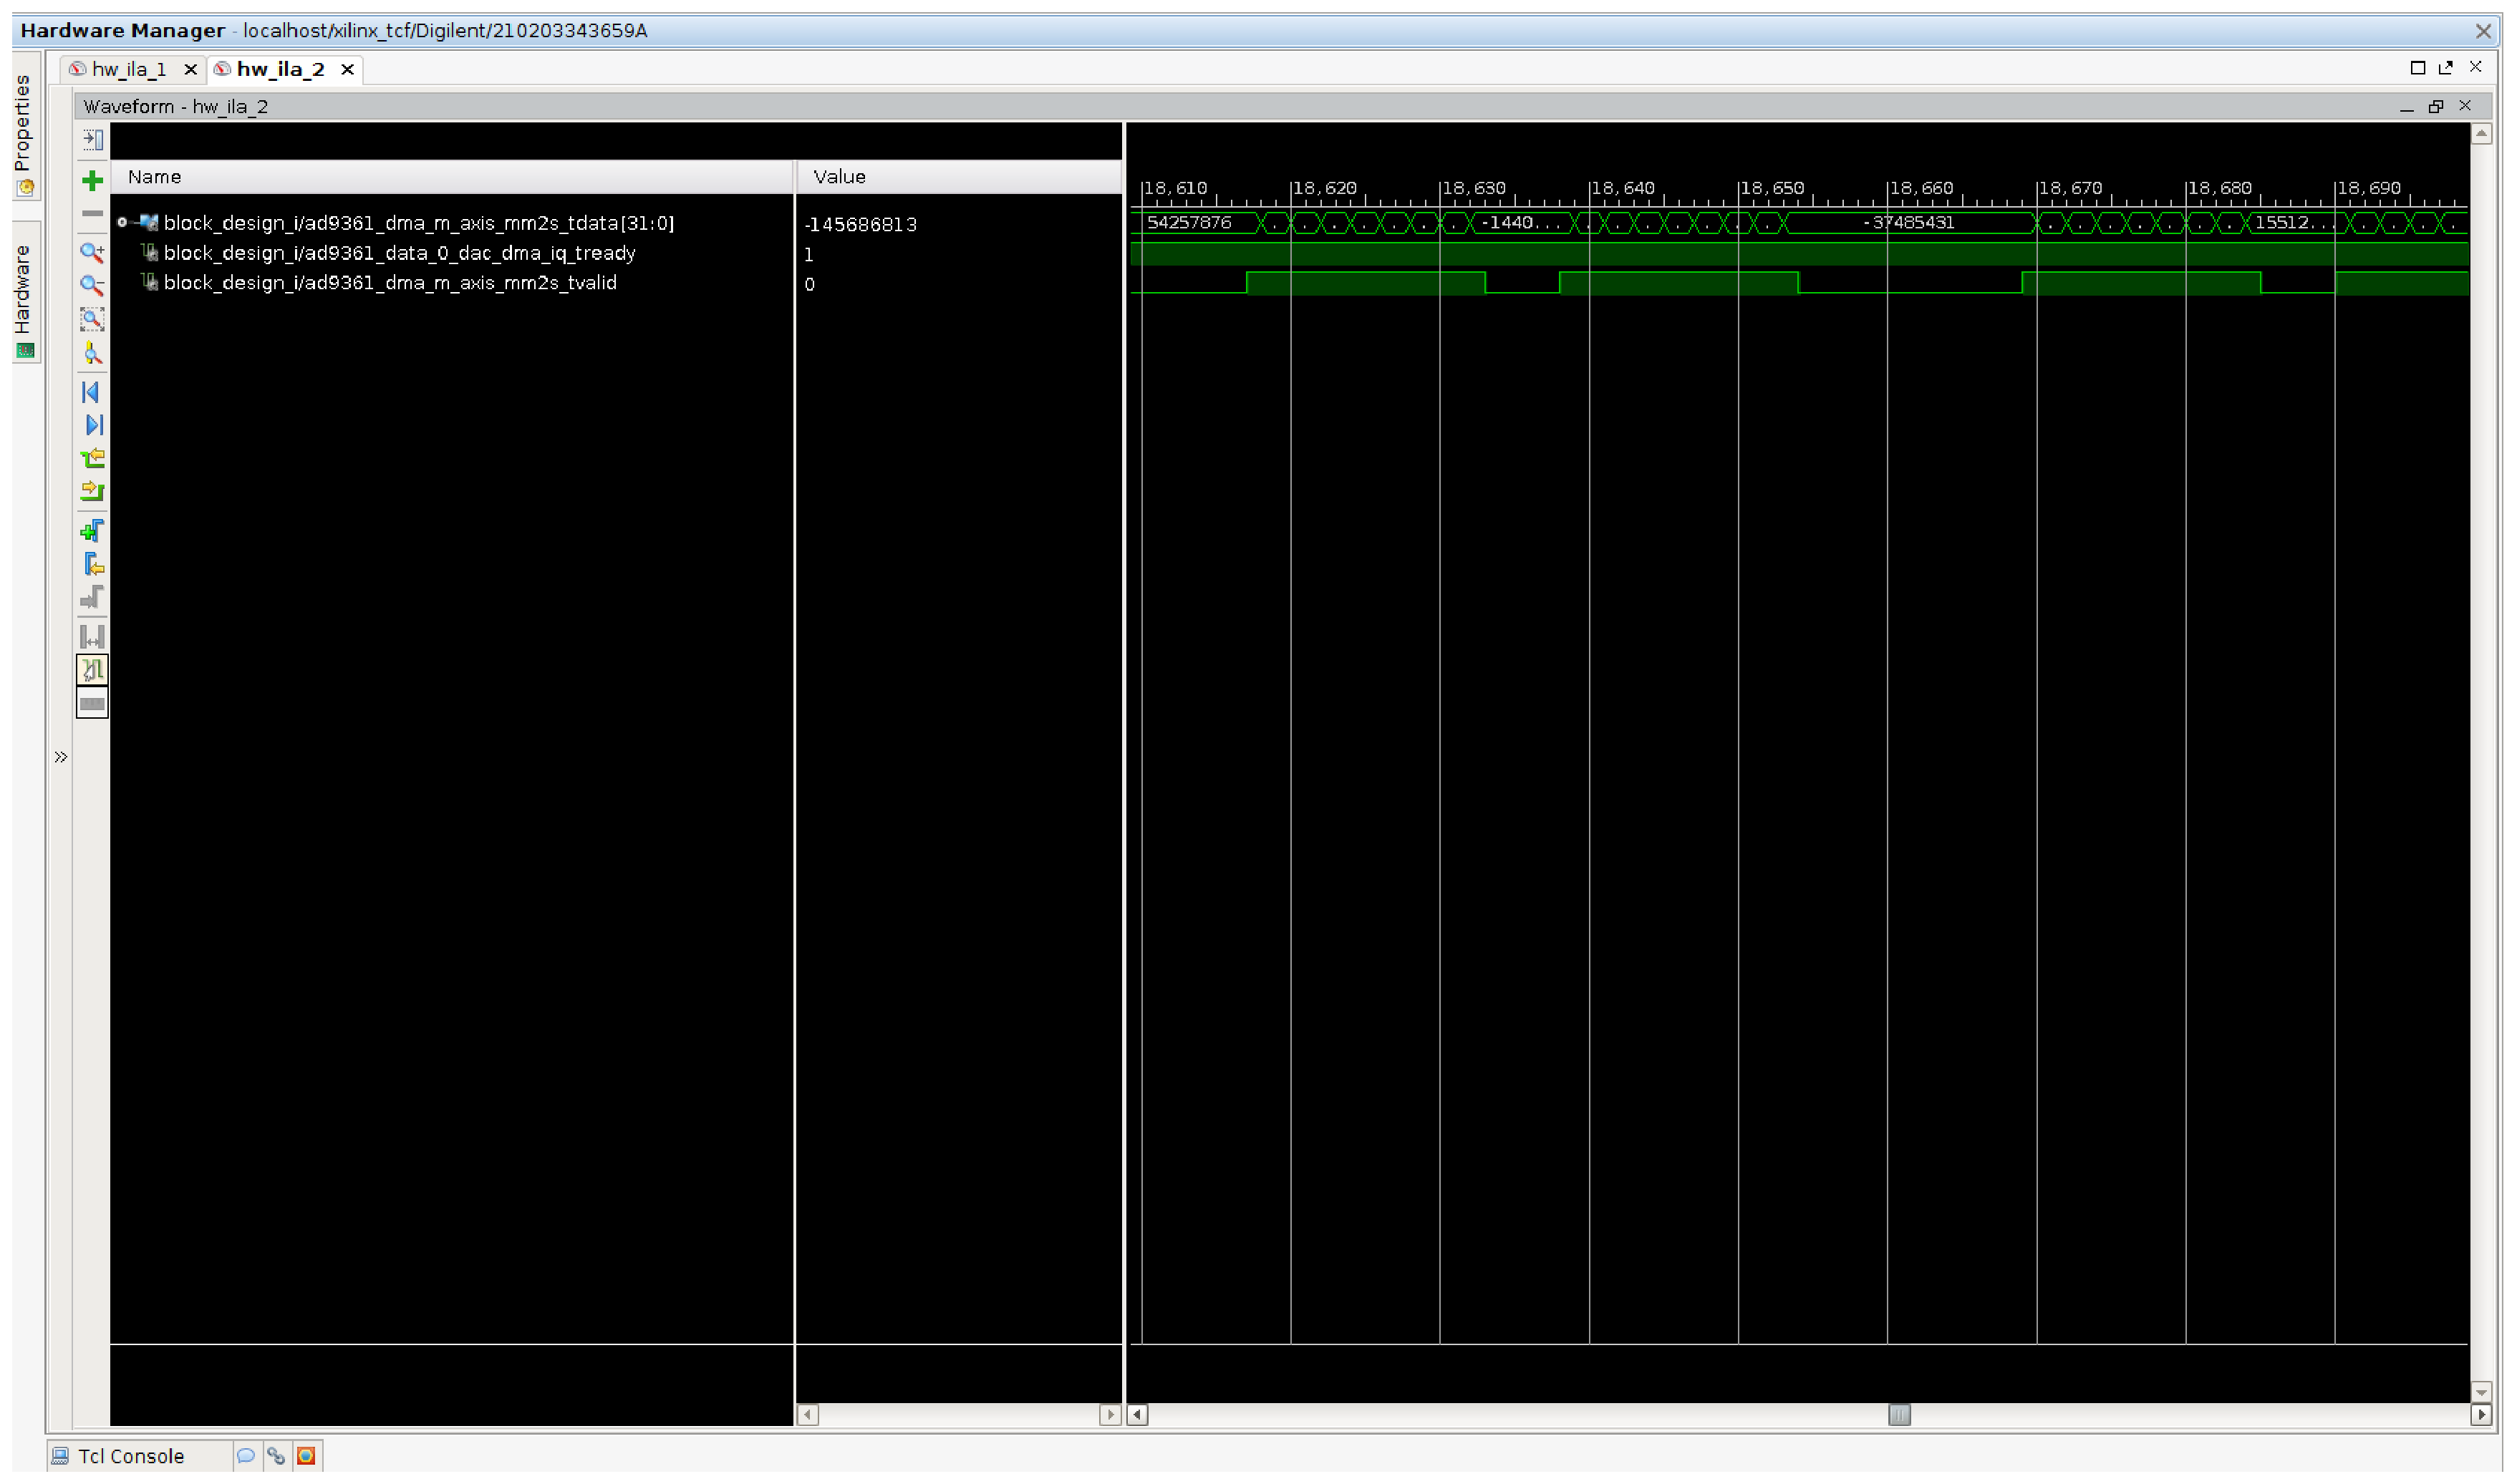
\includegraphics[width=0.85\textwidth]{./figures/ila_dataflow}
    \caption{ Digital Data read from memory by DMA.
    \label{fig:dataflowdig}}
\end{figure}

\begin{figure}[htbp]
    \centering
    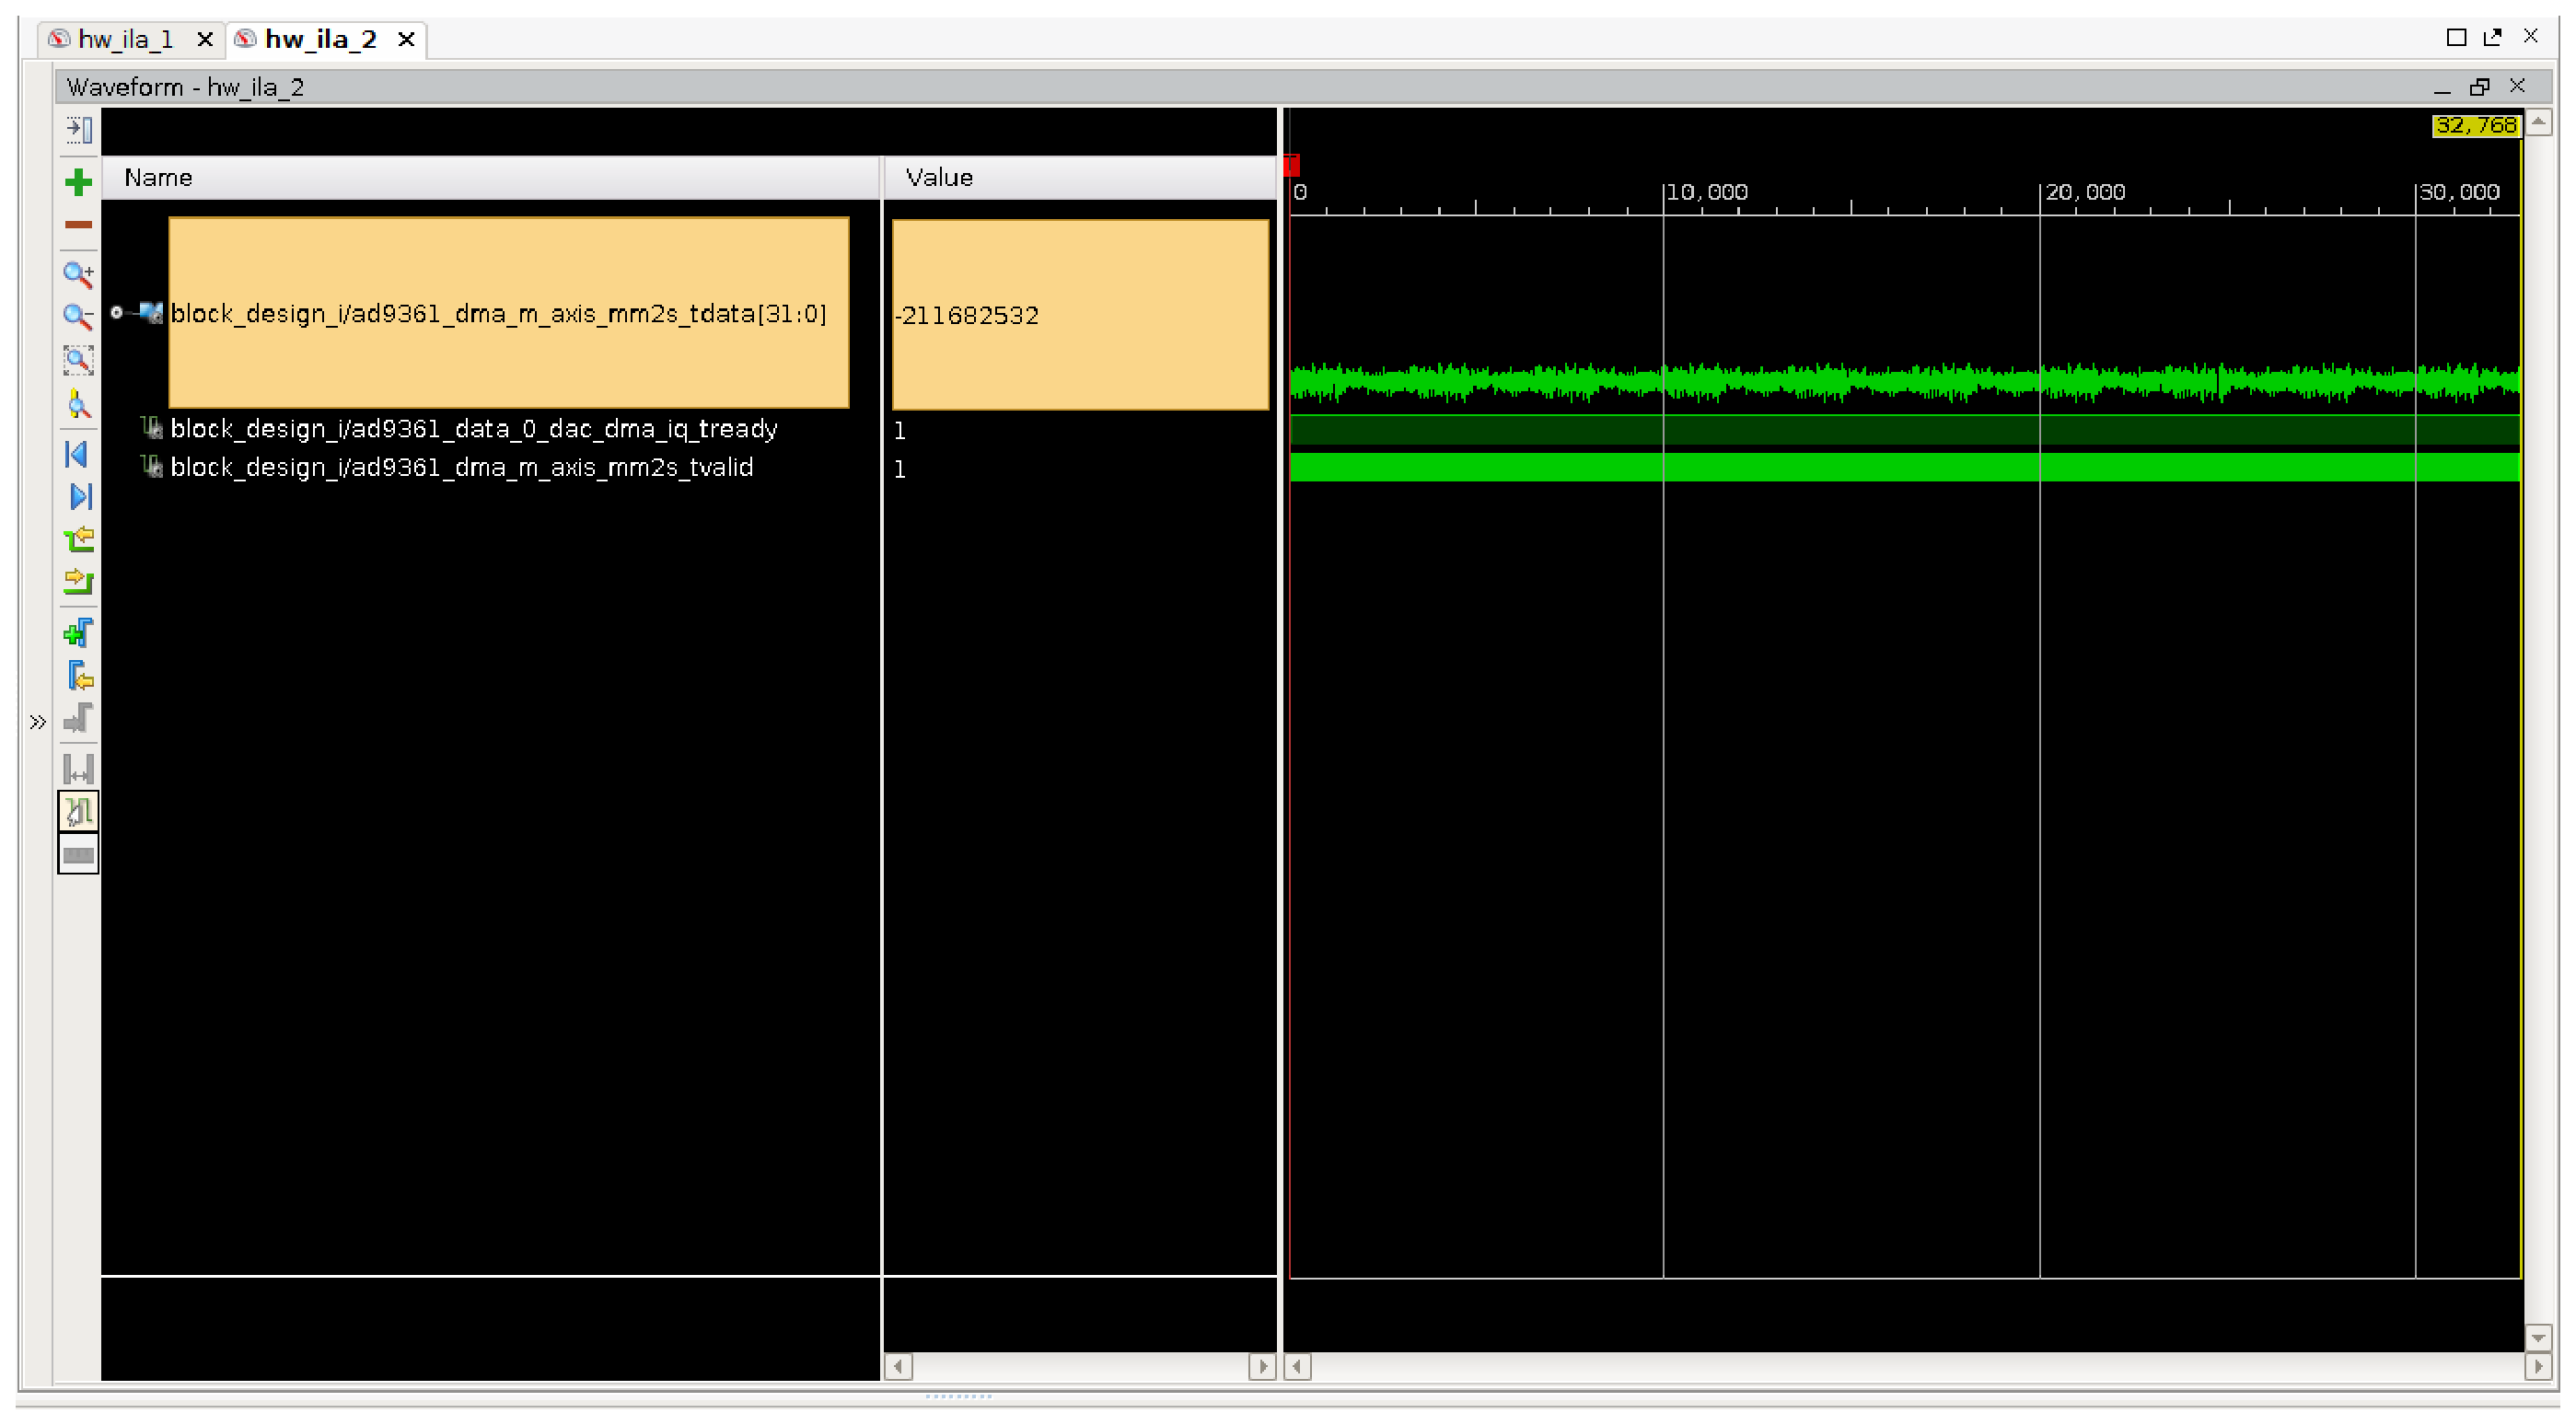
\includegraphics[width=0.85\textwidth]{./figures/ltedac_ila}
    \caption{ Analog form Data read form memory by DMA.
    \label{fig:dataflowana}}
\end{figure}

\begin{figure}[htbp]
    \centering
    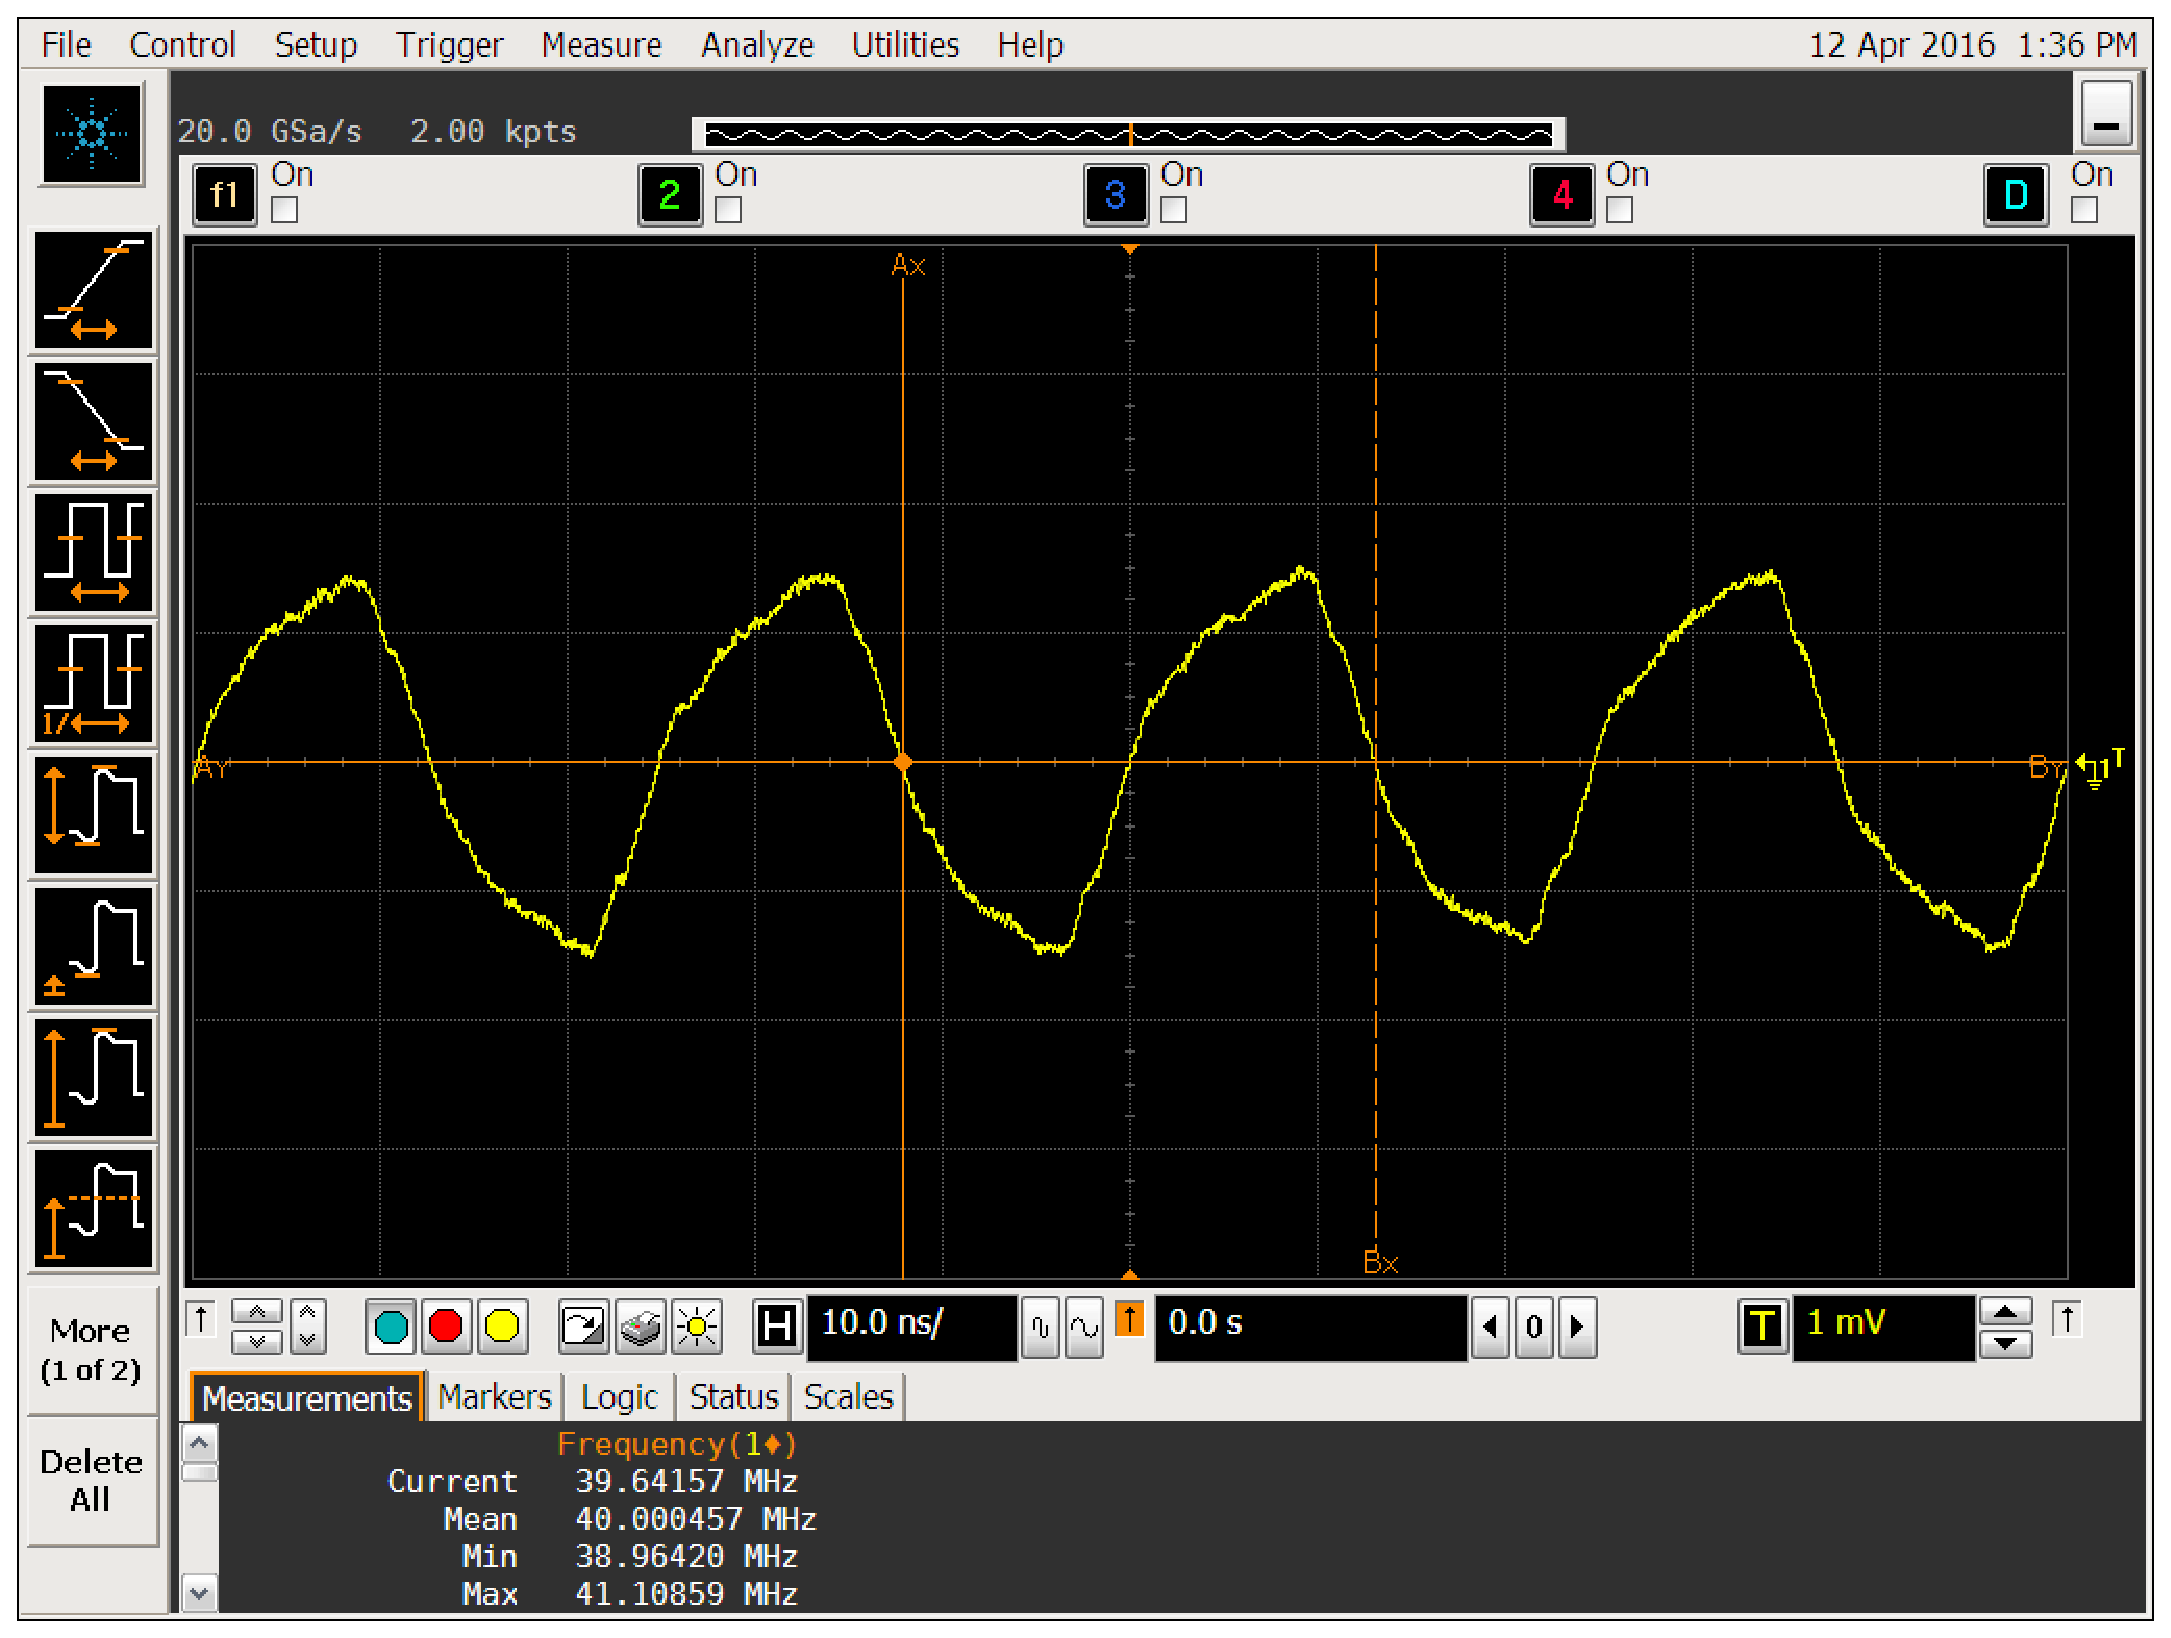
\includegraphics[width=0.85\textwidth]{./figures/oscill_ad9361_dac_clk}
    \caption{ DAC Clock Output
    \label{fig:dacclk}}
\end{figure}

\begin{figure}[htbp]
    \centering
    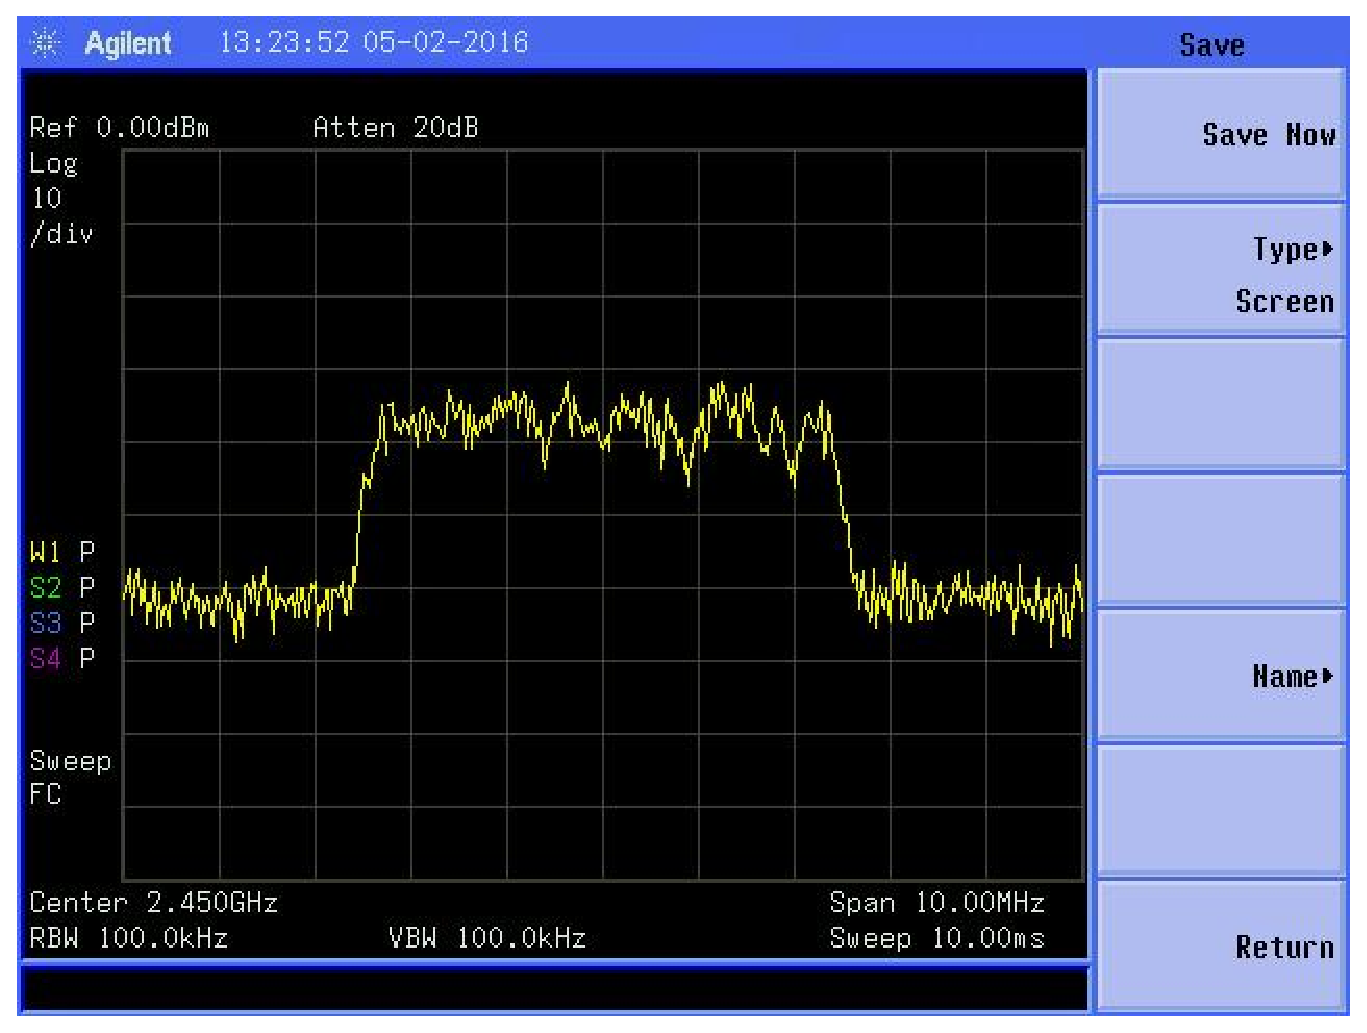
\includegraphics[width=0.85\textwidth]{./figures/lte_5m}
    \caption{ LTE signal output from FMComms2 Spectrum
    \label{fig:lte5m}}
\end{figure}

\vfill
\clearpage

\section{Reception Tests (ADC)}
\label{result:adc}

\begin{figure}[htbp]
    \centering
    \includegraphics[width=0.85\textwidth]{./figures/dac_signals}
    \caption{ DAC signals controlling data writing
    \label{fig:adcsignals}}
\end{figure}

\vfill
\clearpage

\section{Optimum Results}
\label{result:optimum}

The expected transmission of lTE signals are below demonstrated by the Analog
Devices IIO scope application.

\begin{figure}[htbp]
    \centering
    \includegraphics[width=0.65\textwidth]{./figures/lte_spectrum_iio}
    \caption{ LTE Spectrum
    \label{fig:ltespectrumiio}}
\end{figure}

\begin{figure}[htbp]
    \centering
    \includegraphics[width=0.65\textwidth]{./figures/lte_constellation_iio}
    \caption{ LTE Constellation
    \label{fig:lteconstellationiio}}
\end{figure}

\begin{figure}[htbp]
    \centering
    \includegraphics[width=0.85\textwidth]{./figures/lte_evm_iio}
    \caption{ LTE EVM
    \label{fig:lteevmiio}}
\end{figure}

\vfill
\clearpage


\part{Conclusion and Future Work}
\chapter{Conclusion}
\label{chap:conclusion}

\section{Conclusion}
\label{sec:conclusion}

The development of this setup was meant to be general and be used in both
research and academic environments. The process of implementing this setup went
through a myriad of fields in telecommunications and embedded systems, such as
communication protocols, embedded programming, electronics and many others,
being this setup a testbed for more complex processes inside the LTE band saves
a lot of time in development. \\

The FMComms2 board allows real-time and scalable change in parameters by
software or hardware signals, and it re-calibrates and reconfigures itself if
needed so, which makes a very good transceiver board to be used in a C-RAN
environment.\\

This setup was extensively documented and can be used in digital communication
classes to show how a real radio frontend system is made, of course there is
much to improve, there is no dynamic clock synchronization between the FPGA and
the FMComms2, there is no communication protocol between the FPGA (BBP) and the
external world other than the FMComms2 such things are necessary to have a real
frontend but were outside the scope of this project which was just to evaluate a
setup for a scalable and dynamically configurable frontend.\\

Although the FMComms2 and the FPGA operates on different clocks, thus no real
synchronization was implemented, this setup has the minimal capability of
transmitting and receiving signals and reconfigure itself on real-time, the main
goal of this work was reached, however there is much to explore with these tools
and devices.

\section{Future Works}
\label{sec:futurew}

Having finished this part of the work a natural sequel would be implementing
Ethernet connection driver in the FPGA, making it possible to receive data from
Ethernet and hand this to the transceiver board following the schematic on
figure \ref{fig:setupeth} idea. This would be a challenge because there is a lot
of things to consider, but the most problematic of them all is synchronization,
the clock in which everything inside the FPGA works is different from the AD9361
clock not only in frequency but in phase, this can bring a lot of problems,
however there is the possibility of feeding FMComms2 with an external clock
which would increase its performance.\\

With Ethernet it would be possible to generate the modulated samples and send
them trough air, just like Gnuradio + USRP and thus demodulate the received back
samples in the PC, however there is another possibility, modulation and
demodulation blocks implemented in the FPGA logic, thus much faster than the PC
ones and with partial reconfiguration there is the advantage of loading various
schemes of modulation/demodulation in the FPGA, implementing thus a very good
SDR. The Ethernet connection, is also very interesting for C-RAN
environment, because Ethernet is cheap and easy to implement.\\

\begin{figure}[htbp]
    \centering
    \includegraphics[width=0.95\textwidth]{./figures/eth_setup}
    \caption{ Setup Enhanced with Ethernet Connection
    \label{fig:setupeth}}
\end{figure}


%%%%%%%%%%%%%%%%%%%%%%%%%%%%%%%%%%`
%   Referencias bibliograficas   %
%%%%%%%%%%%%%%%%%%%%%%%%%%%%%%%%%%

\renewcommand\bibname{References}
%\bibliographystyle{../../../public/ABNT-20020112}
%\bibliographystyle{../public/IEEEtran}
%\bibliographystyle{../../../Public/IEEEtran_pt}
\bibliographystyle{abnt}
\bibliography{references}

%temorary tag just while there is no \citation
%eliminates no \citation error
\nocite{*}

\clearpage

%%%%%%%%%%%%%%%%%%%%%
%   Appendix        %
%%%%%%%%%%%%%%%%%%%%%

%\appendix
%\input{appendix/append_pll}
%\input{appendix/append_fpga_flow}
%\chapter{AD9361 NO-OS Driver}
\label{app:noos}


\begin{table}[]
\centering
\caption{ad9361 Base Configuration}
\label{tab:basecf}
\begin{tabular}{|l|l|l|}
\hline
\textbf{Linux Device Tree Attribute}               & \textbf{No-OS AD9361\_ParamInit structure member}  & \textbf{Description}                              \\ \hline
adi,2rx-2tx-mode-enable                   & two\_rx\_two\_tx\_mode\_enable            & Use 2Rx2Tx mode - default 1Rx1Tx (AD9364 must clear this)           \\ \hline
adi,frequency-division-duplex-mode-enable & frequency\_division\_duplex\_mode\_enable & Use FDD mode - default TDD                                          \\ \hline
adi,tdd-use-dual-synth-mode-enable        & tdd\_use\_dual\_synth\_mode\_enable       & In TDD mode use Dual Synth mode - default only one Synth is enabled \\ \hline
adi,tdd-use-fdd-vco-tables-enable         & tdd\_use\_fdd\_vco\_tables\_enable        & In TDD mode use the FDD VCO tables                                  \\ \hline
adi,tdd-skip-vco-cal-enable               & tdd\_skip\_vco\_cal\_enable               & Option to skip VCO cal in TDD mode when moving from TX/RX to Alert  \\ \hline
\end{tabular}
\end{table}

\begin{table}[]
\centering
\caption{ENSM Control}
\label{tab:ensm}
\begin{tabular}{|l|l|l|}
\hline
\textbf{Linux Device Tree Attribute}                  & \textbf{No-OS AD9361\_ParamInit structure member}      & \textbf{Description}                                                                \\ \hline
adi,ensm-enable-pin-pulse-mode-enable                 & ensm\_enable\_pin\_pulse\_mode\_enable                 & ENSM control Pins (ENABLE/TXNRX) use Pulse mode - default Level Mode                \\ \hline
adi,ensm-enable-txnrx-control-enable                  & ensm\_enable\_txnrx\_control\_enable                   & ENSM control Pins (ENABLE/TXNRX) control ENSM state - default SPI writes            \\ \hline
adi,frequency-division-duplex-independent-mode-enable & frequency\_division\_duplex\_independent\_mode\_enable & Use independent FDD mode - allows individual control over RX and TX (Pin Mode Only) \\ \hline
\end{tabular}
\end{table}

\begin{table}[]
\centering
\begin{adjustbox}{width=1\textwidth}
\label{my-label}
\begin{tabular}{|l|l|l|}
\hline
\textbf{Linux Device Tree Attribute}         & \textbf{No-OS AD9361\_ParamInit structure member} & \textbf{Description}                                                                   \\ \hline
adi,rx-synthesizer-frequency-hz              & rx\_synthesizer\_frequency\_hz                    & RX LO power-up Frequency in Hz                                                         \\ \hline
adi,tx-synthesizer-frequency-hz              & tx\_synthesizer\_frequency\_hz                    & TX LO power-up Frequency in Hz                                                         \\ \hline
adi,tx-fastlock-delay-ns                     & tx\_fastlock\_delay\_ns                           & TX fastlock delay in ns                                                                \\ \hline
adi,rx-fastlock-delay-ns                     & rx\_fastlock\_delay\_ns                           & RX fastlock delay in ns                                                                \\ \hline
adi,rx-fastlock-pincontrol-enable            & rx\_fastlock\_pincontrol\_enable                  & RX fastlock pin control enable                                                         \\ \hline
adi,tx-fastlock-pincontrol-enable            & tx\_fastlock\_pincontrol\_enable                  & RX fastlock pin control enable                                                         \\ \hline
adi,trx-synthesizer-target-fref-overwrite-hz & trx\_synthesizer\_target\_fref\_overwrite\_hz     & This allows forcing a lower F\_REF window (worse phase noise, better fractional spurs) \\ \hline
adi,external-tx-lo-enable                    & external\_tx\_lo\_enable                          & Enables external LO for TX                                                             \\ \hline
adi,external-rx-lo-enable                    & external\_rx\_lo\_enable                          & Enables external LO for RX                                                             \\ \hline
\end{tabular}
\end{adjustbox}
\caption{lol}
\end{table}


%%%%%%%%%%%%%%%%%%%%%
%   blank page      %
%%%%%%%%%%%%%%%%%%%%%

\newpage
\thispagestyle{empty}
\mbox{}

%% -- Termino do TCC
\end{document}
